\documentclass[a4j]{jsbook}

\usepackage[dvipdfmx]{graphicx}
\usepackage[top=20truemm,bottom=20truemm,left=30truemm,right=20truemm]{geometry}
\usepackage{amsmath, amssymb}
\usepackage{bm}
\usepackage{fancybox}
\usepackage{here}
%\usepackage{boxedminipage}
\usepackage{eclbkbox}
%\usepackage{ascmac}
%\usepackage{enumerate}
\usepackage{tcolorbox}
\usepackage{hyperref}

%\renewcommand{\bibname}{参考文献}
%\bibliographystyle{junsrt}

\newcommand{\admin}{{\tt compexp@exa.phys.s.u-tokyo.ac.jp}}
\newcommand{\nendo}{2018}

\newcommand{\til}{\char`\~}
\newcommand{\Machine}{{\tt exp-xs00}}
\newcommand{\MachineFull}{{\tt alps.phys.s.u-tokyo.ac.jp}}
\newcommand{\promptn}{\$}
\newcommand{\prompt}{\$ }
\newcommand{\promptECC}{[s001500@ecc\$ }
\newcommand{\shellname}{bash}
\newcommand{\shellbash}{bash}
\newcommand{\pager}{{\bf less}}
\newcommand{\ux}{ux101$>$}
\newcommand{\ctrl}[1]{\ovalbox{\mathstrut ctrl}-\ovalbox{\mathstrut #1}}
\newcommand{\esc}[1]{\leavevmode\ovalbox{\mathstrut Esc}-\ovalbox{\mathstrut #1}}
\newcommand{\ret}{\ovalbox{\mathstrut Enter}}
\newcommand{\spc}{\leavevmode\ovalbox{\mathstrut スペース}}
\newcommand{\BS}{\ovalbox{\mathstrut Backspace}\ あるいは \ovalbox{\mathstrut Delete}キー}
\newcommand{\cursor}{\vrule height8pt depth3pt width4pt\relax}
\newcommand{\cursorone}{\vrule height8pt depth3pt width4pt\relax}
\newcommand{\cursortwo}{\vrule height8pt depth3pt\relax}
\newcommand{\destroymenu}{右}
\newcommand{\rloginmenu}{真ん中}
\newcommand{\killmenu}{Destroy window}
\newcommand{\itemf}[1]{\item {\bf #1}}

%\usepackage[T1]{fontenc}
%\usepackage{tgpagella}
%\usepackage{dtklogos}

\newsavebox{\fminibox}
\newenvironment{myframe}[2][\textwidth]%
{\vspace{12pt}\newline\begin{minipage}{#1}\textbf{#2}\newline%
    \begin{lrbox}{\fminibox}\begin{minipage}{#1}}%
{\end{minipage}\end{lrbox}\fbox{\usebox{\fminibox}}\end{minipage}\vspace{12pt}}

\newenvironment{myframe2}[1]{%
  \vspace{12pt}%
  \begin{breakbox}%
  {\parindent=0pt\textbf{\underline{#1}}}%
}{%
  \end{breakbox}\vspace{12pt}%
}

\newenvironment{myframe3}[1]{%
  \vspace{12pt}%
  {\parindent=0pt\textbf{\underline{#1}}}\quad%
}{%
  \vspace{12pt}
}

%%% 例環境
\newcounter{reidai}[section]
\def\thereidai{\thesection.\arabic{reidai}.}
\newenvironment{reidai}{%
  \refstepcounter{reidai}%
  \begin{myframe2}{例 \thereidai}%
  \baselineskip=12pt%
  \begin{quote}%
}{%
  \end{quote}%
  \end{myframe2}%
}

\newcounter{kekka}[section]
\def\thekekka{\thereidai}
\newenvironment{kekka}%
{\refstepcounter{kekka}
  \begin{myframe2}{結果 \thekekka}
  \baselineskip=12pt%
  \begin{quote}%
}{%
  \end{quote}%
  \end{myframe2}%
}


%%% 練習環境
\newenvironment{commandline2}{%
  %\begin{quote}
  \begin{tcolorbox}\tt%
}{%
  \end{tcolorbox}%
  %\end{quote}%
}

\newcounter{renshuu}[section]
\def\therenshuu{\thesection.\arabic{renshuu}.}
\newenvironment{renshuu}{%
  \refstepcounter{renshuu}%
  \begin{myframe3}{練習 \therenshuu}%
}{%
  \end{myframe3}%
}

\newenvironment{renshuu-answer}[1]{%
  \begin{myframe2}{練習 \ref{#1}}
  \begin{quote}%
}{%
  \end{quote}%
  \end{myframe2}%
}

\newcommand{\esckey}{{\tt \ovalbox{Esc}}}
\newcommand{\tabkey}{{\tt \ovalbox{Tab}}}
\newcommand{\typecom}[2][\ret]{\begin{quote}{\tt\prompt \underline{#2} }#1\end{quote}}
\newcommand{\typeans}[1]{\begin{quote}\tt#1 \end{quote}}

\def\clangpara#1{\paragraph{#1}\mbox{}\\}

%% \newcounter{reidaii}[section]
%% \def\thereidaii{\thesection.\arabic{reidaii}.}
%% \newenvironment{reidaii}%
%% {\refstepcounter{reidaii}%
%%   \begin{myframe}{例題 \thereidaii}}%
%% {\end{myframe}}

%% \newcounter{kekkai}[section]
%% \def\thekekkai{\thereidaii}
%% \newenvironment{kekkai}%
%% {\refstepcounter{kekkai}
%%   \begin{myframe}{結果 \thekekkai}}%
%% {\end{myframe}}

\newenvironment{commandline}%
{\vspace{6pt}\newline\hspace{26pt}\begin{minipage}{\textwidth}}%
{\end{minipage}\vspace{6pt}}

\makeatletter
\@addtoreset{equation}{section}
\makeatother

\def\labelitemi{$\Rightarrow$}

%
% for algorithm
%

\newcommand{\pard}[3]{\frac{\partial^{#1}#2}{\partial #3^{#1}}}
\newcommand{\normv}[1]{\lvert \bm{#1} \rvert}

\newcommand{\shusseki}{\textbf{shusseki@nt.phys.s.u-tokyo.ac.jp}}



\pagestyle{plain}

\begin{document}
\thispagestyle{empty}
\pagestyle{empty}
\begin{titlepage}
\vspace*{5cm}
\begin{center}
{\Huge\bf 計算機実験ハンドブック}\\
\vspace*{14cm}
{\LARGE\bf \nendo 年度}\\
\vspace{1.0cm}
{\LARGE\bf 東京大学理学部物理学科}
\end{center}
\end{titlepage}
\clearpage
\pagestyle{plain}
\cleardoublepage

\setcounter{page}{1}
\setcounter{tocdepth}{3}
\tableofcontents
\cleardoublepage

\chapter{はじめに}
%\section{はじめに}

理学部物理学科3年の講義「計算機実験I」および「計算機実験II」は、理論・実験を問わず、学部〜大学院〜で必要とされる現代的かつ普遍的な計算機の素養を身につけることを目標としている。
基礎的な数値計算アルゴリズムとその応用を学習するだけでなく、実習を通じて、計算機の操作、C言語を用いたプログラミング技術、\LaTeX による科学論文の作成技術などを学ぶ。

本冊子は、「計算機実験I」および「計算機実験II」の時間に、より効果的に実習を進めることができるよう、必要とされる技術的な点をまとめたものである。
大いに役立てて欲しい。
また、間違いや不明な点などがある場合には、担当教員、あるいはティーチングアシスタントまでぜひ知らせてほしい。

実習は主として教育用計算機システムECCSの端末(iMac)を用いるが、iMacへのログイン方法や基本的な操作方法、Webやメールの利用方法などについては、本書では触れていない。
教育用計算機システムの「利用の手引」(http://www.ecc.u-tokyo.ac.jp/guide/current/)に詳しい解説があるので、そちらを参照のこと。


\chapter{UNIX入門}
%\nocite{Sakamoto1993}

この章では、UNIXと呼ばれるOS (オペレーティングシステム)の操作法について学ぶ。通常、Mac OS XやWindowsでは、マウスを使って画面を操作する。実は、Mac OS Xの内部ではDarwinと呼ばれるUNIX系のOSが動作しており、「ターミナル」アプリケーションを立ち上げることにより、UNIXの様々な機能に直接アクセスすることができる。また、ワークステーションやスーパーコンピュータなど、より大きな規模の計算を行うことのできる計算機も、ほぼ全てLinuxなどのUNIX系OSである。

UNIX系のOSの特徴としては、シンプル、柔軟かつオープンであり、ネットワークに強いことが挙げられる。シェルやスクリプト言語を組み合わせることにより、簡単なコマンドで複雑な処理を実現することができる。また、ネットワーク経由で使用することが前提となっており、実際に計算機がどこにあるかを意識することなしに、透過的に利用できる。UNIXを取得することにより、目の前のPCだけでなく世界中の計算機を利用することが可能となり、計算能力が一気に増えることになる。

\section{UNIX のコマンド}

この節での操作はすべて、ターミナル(「シェル」とも呼ぶ)内でコマンドを打ち込み、最後にリターンキーを押すことより実行する。確実に操作できるまで、繰り返し練習してほしい。下線を引いた部分がキーボードからの入力である。行頭の``\texttt {\promptn}''はプロンプトと呼ばれる。UNIXのシェルがユーザからのコマンド入力待ちの状態であることを示すものであり、コマンド入力時にタイプする必要はない。

\subsection{ファイルの操作}
\label{sec:unix:fileManagement}
この節では、ファイルを作ったり、消したりといった基本的な操作を紹介する。ファイルというのは計算機が情報を書き込むための一つの単位である。ファイルには名前を付けることができて、その名前を指定することでファイルを編集したり消したりできる。

%% %\newpage

\subsubsection{ファイルの基本操作}
ファイルをコピーするには{\tt cp}コマンド({\bf c}o{\bf p}yの略)を用いる。例えば、コマンドラインで
\begin{commandline2}
\prompt \underline{cp /usr/local/example/circle.c circle.c}
\end{commandline2} \noindent
を実行すると、{\tt /usr/local/example}という名前のディレクトリにあるファイル{\tt circle.c}が、カレントディレクトリにコピーされる。{\tt /usr/local/example/circle.c}の部分がコピー元に対応し、後の{\tt circle.c}がコピー先を意味する。コピー先がディレクトリの場合には、コピー先のディレクトリにコピー元と同じ名前のファイルが作られる。したがって、上の例は、カレントディレクトリを表す ``{\tt .}'' を用いて、
\begin{commandline2}
\prompt \underline{cp /usr/local/example/circle.c .}
\end{commandline2} \noindent
としても同じ結果となる。元とは異なる名前でコピーしたい場合には、
\begin{commandline2}
\prompt \underline{cp /usr/local/example/circle.c oval.c}
\end{commandline2} \noindent
などとする。同じ名前のファイルがすでに存在する場合には上書きされるので注意せよ。

ここで、{\tt ls}コマンド({\bf l}i{\bf s}tの略)を実行すると
\begin{commandline2}
\prompt \underline{ls}
\vspace*{-.8em} 
\begin{verbatim}
Desktop    circle.c
\end{verbatim}
\end{commandline2} \noindent
と表示され、正しくコピーされたことが分かる。このように、{\tt ls}コマンドを使うことで、どのようなファイルがあるのかを知ることができる。さらに、{\tt ls -l}を実行すると
\begin{commandline2}
\prompt \underline{ls -l}
\vspace*{-.8em} 
\begin{verbatim}
total 2
drwxr-xr-x  2 s001500 student      512 Apr 16 03:40 Desktop
-rw-r--r--  1 s001500 student      372 Apr 16 03:43 circle.c
\end{verbatim}
\end{commandline2} \noindent
のように、より詳細な情報\footnote{表示の1行目は、左端の {\tt d} が、そのファイルがディレクトリであることを示し、次の{\tt rwx}はファイルの所有者が読み取り可能({\tt r})、書き込み可能({\tt w})、実行可能({\tt x})であることを示している。(ディレクトリが読み取り可能であるとは、そのディレクトリにどのようなファイルが入っているかを{\bf ls}コマンドで調べられることをいい、ディレクトリが書き込み可能とは、そのディレクトリに新しくファイルやディレクトリを新しく作ったり、すでにあるファイルなどを消したりできることをいう。さらに、ディレクトリが実行可能であるとは、そのディレクトリ内部のファイルを操作できたり、そのディレクトリに移動するとか、そのディレクトリの名前をパスに含めることができることを意味する。) 次の{\tt r-x}は同じグループ(学生はすべて同じグループに属する)に所属する人が、読み取りと実行可能であることを示し、その次の{\tt r-x}はそのほかすべての人が読み取りと実行可能であることを示している。隣のカラムの{\tt s001500}は、そのファイルの所有者が{\tt s001500}であることを示し、次のカラムは所有グループを示している。次の{\tt 512}は、そのファイルの大きさが512 byteであることを示している。{\tt Apr 16 03:40}は、そのファイルに最後に変更を加えた日時を示す。そして最後がファイルの名前である。}を得ることができる。この{\tt -l}をオプション(あるいはコマンドラインオプション)と呼ぶ。{\tt ls}コマンドには他にも様々なオプションが用意されている。{\tt -F} オプションをつければ、ファイルの名前の後にファイルの種別を表す文字をつけてくれる。ディレクトリには {\tt /} が、実行可能ファイルには{\tt $ \ast$} がつく。{\tt -R} オプションをつければ、カレントディレクトリ以下のすべてのディレクトリの中身を見ることができる。また、{\tt -a} とすると、通常表示されない . (ピリオド)から始まるファイルも見ることができるようになる。

次にファイルの名前を変えてみよう。先の{\tt circle.c}を{\tt ring.c}に名前を変更するには、{\tt mv}コマンド({\bf m}o{\bf v}eの略)を使う。
\begin{commandline2}
\prompt \underline{mv circle.c ring.c}
\end{commandline2} \noindent
{\tt ls}コマンドで実際に名前が変更されたか確かめてみよう。

続いて{\tt rm}コマンド({\bf r}e{\bf m}oveの略)を用いてファイルを消してみよう。
\begin{commandline2}
\prompt \underline{rm ring.c}
\end{commandline2} \noindent
{\bf 一度消したファイルは二度と復旧できない}ので慎重に実行しなければならない。自信がないなら、
\begin{commandline2}
\prompt \underline{rm -i ring.c}
\end{commandline2} \noindent
のように{\tt -i}オプションをつけるとよい。ファイルごとに消してよいかどうかの確認をしてくれるので安心である。

さて、ここまでディレクトリという言葉が何度か出てきた。UNIXでは、ディレクトリという特殊なファイルを使って、たくさんのファイルをtree状に管理することができる。ディレクトリとは書類をまとめる書類箱だと思えばよいだろう。ときに大きな書類箱のなかに小さな書類箱が入っていることもあるわけで、ディレクトリの中にディレクトリがあってもいっこうに構わない。

ログインして最初にいるディレクトリのことをホームディレクトリと呼ぶ。今いるディレクトリ\footnote{カレントディレクトリ、あるいはワーキングディレクトリと呼ぶ。}がどこかを知るには、{\tt pwd}コマンド({\bf p}rint {\bf w}orking {\bf d}irectoryの略)を使う。{\tt /home/s001500} と表示されれば ルートディレクトリ\footnote{ルートディレクトリとは一番上のディレクトリのことであり、最初の{\tt /}がルートディレクトリを表す。}の下の {\tt home} というディレクトリの下の、{\tt s001500}というディレクトリにいるということが分かる。

試しに{\tt sample}という ディレクトリを作ってみよう\footnote{すでにあるディレクトリを消すには{\tt rmdir}コマンド({\bf r}e{\bf m}ove {\bf dir}ectoryの略)を使う。{\tt rmdir} でディレクトリを消すときはそのディレクトリの中にファイルやディレクトリが1つもない状態になっていなくてはならない。消したいディレクトリの中にファイルが残っているときは {\tt rm} コマンドを使い、ディレクトリが残っているときは {\tt rmdir} コマンドを使う。残っているファイルやディレクトリをいちいち消すのが面倒な場合は{\tt rm -r {\it directory}}とすれば、{\it directory}の中に何が残っていてもすべてきれいに消し去ってくれる。}。
\begin{commandline2}
\prompt \underline{mkdir sample}
\end{commandline2} \noindent
これで{\tt sample}というディレクトリが作成された。{\tt ls}コマンドで確かめてみよう。次に、今作ったディレクトリに移動してみよう。
\begin{commandline2}
\prompt \underline{cd sample}
\end{commandline2} \noindent
{\tt cd}は{\bf c}hange {\bf d}irectoryの略である。ここで、先ほどの {\tt cp}コマンドを使えば、このディレクトリにファイルをコピーすることができる。さらにこの中で\underline{{\tt mkdir chap4}}と打てば、{\tt sample}ディレクトリの下に{\tt chap4}ディレクトリが作成される。

では、元のディレクトリに戻るにはどうすればよいのだろうか? それには
\begin{commandline2}
\prompt \underline{cd ..}
\end{commandline2} \noindent
を実行する。{\tt cd}と{\tt ..}の間に空白があることに注意すること。

ツリー構造の中で、どのようにディレクトリやファイルを指定すればよいのだろうか。ディレクトリのツリーを図示すれば次のようになる。

\unitlength 1mm
\begin{picture}(100,85)(-30,-75)
\put(50,0){\fbox{/}}
\put(50,-5){\line(-2,-1){23}}\put(50,-5){\line(0,-1){13}}\put(50,-5){\line(2,-1){23}}
\put(25,-20){\fbox{home}}\put(47,-20){\fbox{usr}}\put(70,-20){\fbox{etc}}
\put(30,-24){\line(-2,-1){23}}\put(30,-24){\line(0,-1){12}}\put(30,-24){\line(2,-1){23}}
\put(0,-40){\fbox{hirano}}\put(25,-40){\fbox{s001500}  ...  }\put(50,-40){\fbox{s815xx} ....}
\put(28,-43){\line(-2,-1){23}}\put(28,-43){\line(0,-1){10}}\put(28,-43){\line(2,-1){23}}
\put(0,-56){\fbox{ftp}}\put(25,-55){\fbox{sample}}\put(50,-55){\fbox{tmp} ... }
\put(28,-58){\line(-2,-1){23}}\put(28,-58){\line(0,-1){10}}
\put(0,-72){\fbox{chap4}}\put(25,-72){\fbox{chap5} ... }
\end{picture}

\noindent このツリーの中の位置は、一番上の {\tt /} で表されるルートディレクトリから順にたどることより指定することができる。これを「絶対パス」と呼ぶ。あるいは、今いるディレクトリ(カレントディレクトリ)からの相対的な位置で指定する方法もある。これを「相対パス」と呼ぶ。例えば、ホームディレクトリの下の{\tt sample}の下の{\tt chap4}ディレクトリは、絶対的な指定では
\begin{tt}
/home/s001500/sample/chap4
\end{tt}
と書かれるが、カレントディレクトリがホームディレクトリの場合、相対的な指定では{\tt sample/chap4}と書かれる。そのディレクトリの中にあるファイルも {\tt /home/s001500/sample/chap4/circle.c}とか{\tt sample/chap4/circle.c}のように指定することができる。特に一つ上のディレクトリは``{\tt ..}''で、カレントディレクトリは``{\tt .}''であらわされる。つまり先ほどの{\tt sample/chap4/circle.c}は{\tt ./../s001500/sample/chap4/circle.c}と書いても同じものを指す。

これで、自由にディレクトリ間を移動することができるようになった。例えば、すでに使った{\tt ls}コマンドは、{\tt /usr/bin}あるいは{\tt /bin}ディレクトリに格納されている\footnote{\underline{\tt which ls}とすることで、{\tt ls}がどこにあるか調べることができる。}。\underline{\tt cd /usr/bin} として、そこに移動してから\underline{\tt ls}と打ってみよう。たくさんのファイルが置かれているが、{\tt ls} というファイルは見付かっただろうか\footnote{例えば、{\tt treasure.here}という名前のファイルを探したい場合、そのファイルがありそうなディレクトリよりも上のディレクトリに行って、\underline{\tt find . -name treasure.here -print}とする。{\tt find}の直後の {\tt .} (ピリオド)は「そのファイルがありそうなディレクトリより上のディレクトリのパス」を指定する。またファイル名があやふやな場合でも、\underline{\tt find . -name 'tre$\ast$.here' -print}のように$\ast$を任意の文字列として合致するファイルを表示してくれる。{\tt find}はとても多機能である。例えば\underline{\tt find . -name 'tre$\ast$.here' -exec cat \{\} $\backslash$;}のように、探し出したファイルに対してコマンドを実行することもできる。{\tt -exec} 以下の書式は コマンドの引数となるファイル名が\{\}となるように書き、最後に {\tt $\backslash$;} を加えればよい。{\tt -exec} の代わりに {\tt -ok} を使えばコマンドを実行する前に一々聞いて来るので {\tt rm}などを {\tt find} で実行したいときには安心である。\underline{\tt find\ .\ -ctime -1 -print}のように{\tt -ctime}で最終変更期日が1日前以内のものだけ表示させるようなことも可能である。{\tt -ctime}の引数を{\tt +1} にすると最終変更期日が1日以上前のものだけが表示される。}。

なお、\underline{{\tt cd}}とだけ打てば、いつでも自分のホームディレクトリに戻ってくることができる。ホームディレクトリは $\tilde{\ }$ とも表されるので \underline{{\tt cd $\tilde{\ }$}}としても同じである。

\subsubsection{ファイルの中を見る}

さて、肝心のファイルの中身を見るにはどうしたらよいのだろう。ファイルの中身を見るにはいくつかの方法がある。ファイルには大別して、中身を見ることができるテキストファイルと中身を見られないバイナリファイルがある。テキストファイルの中身は、{\tt cat}コマンドで見ることができる\footnote{バイナリのファイルの中身を覗くための{\tt od} ({\bf o}ctal {\bf d}ump)というコマンドもある。}。
\begin{commandline2}
\prompt \underline{cat circle.c}
\end{commandline2} \noindent
{\tt cat}は最も手軽にファイルの中身をのぞくことのできるコマンドである。中身が長すぎる場合、{\tt cat}では流れていってしまうが、
\begin{commandline2}
\prompt \underline{more circle.c}
\end{commandline2} \noindent
と打つことにより、ちょうどよい所で一旦止めてくれる。\fbox{\tt --More--(xx\%)} のような表示が左下に見えたら、\spc を叩いてみよう。次のページが表示されるはずである。\underline{\tt h}と打つと簡単なヘルプが見られる。\underline{\tt b}か\ctrl{B}で1ページ戻る。また\ret で1行進む。さらに、\underline{\tt /}の後に\underline{\tt 文字列}を打つことでファイル中の文字列を検索することができる。検索された文字列を含む行はウインドウの一番上に表示される。\underline{\tt n}と打てばもう一度同じ文字列を探してくれる。また、\underline{\tt 10d}のように数字を入れてから\underline{\tt d}を打てば、その数字分だけ進む。{\tt more}から抜けるには、\underline{\tt q}を入力する。

{\tt more}と似ているが、もう少し使い勝手のよい{\tt less}\label{sect:less}というコマンドもある。{\tt less}では上向きにスクロールすることができる。\underline{\tt j}で一行下に、\underline{\tt k}で一行上\footnote{編集用のソフト {\tt vi} のキー操作と同じ。}に進む。{\tt more}と同じく、スペースバー、\underline{\tt h}、\underline{\tt b}、\underline{\tt d}、\underline{\tt /}、\underline{\tt n}、\underline{\tt q}のようなコマンドも使える。更に \underline{\tt g}でファイルの先頭に、\underline{\tt G}でファイルの最後尾にジャンプすることができる\footnote{{\tt \underline{tail circle.c}}のようにすれば、ファイルの最後だけ見ることができる。また \underline{\tt tail -30}のように指定することで最後から30行目以降を見ることができる。}。

次に、たくさんあるファイルの中に特定の文字列が含まれているか調べてみよう。
\begin{commandline2}
\prompt \underline{grep main $\ast$.c}
\end{commandline2} \noindent
と入力してみよう。どの``{\tt .c}''で終るファイルに main という文字列が含まれているか一目瞭然である\footnote{さらに\texttt{\underline{grep -n printf $\ast$.c}}としてみると、各ファイルの何行目に printf という文字列があるのかが分かる。さらに、\texttt{\underline{grep -n -e $'.\ast$gram.$\ast'$ $\ast$.c}}で、.$\ast$のところに任意の文字列があてはまるすべての文字列について検索する。シングルクォーテーションで囲まなくてはいけない点に注意すること。}。

\subsubsection{ファイルの保護 (1)}
他の人に見られたくないファイルにはプロテクションをかけることができる。
\begin{commandline2}
\prompt \underline{chmod o-r circle.c}
\end{commandline2} \noindent
とすれば自分と、自分と同じグループに属する人以外はそのファイルを見ることができなくなる\footnote{{\tt o}は other の頭文字である。反対に他の人にも見えるようにするには \underline{\tt o-r} を\underline{\tt o+r} に変えて実行する。\underline{\tt chmod u=rwx,g+x,o-r circle.c}のように指定することもできる。そのほか {\tt g} (group) は 同じグループ、{\tt u} (user) は所有者、{\tt a} (all)はユーザーも含めた全員を表し、{\tt r} 、{\tt w} 、{\tt x} はそれぞれ、read, write, execute を表す。}。
\begin{commandline2}
\prompt \underline{chmod g-r circle.c}
\end{commandline2} \noindent
とすれば同じグループの人からも見られなくなる。同じ要領で
\begin{commandline2}
\prompt \underline{chmod o-rwx circle.c}
\end{commandline2} \noindent
とすれば他の人は {\tt circle.c} というファイルを読むことも書き込むことも実行することもできなくなり、
\begin{commandline2}
\prompt \underline{chmod go-rwx sample}
\end{commandline2} \noindent
とすれば自分以外のだれも {\tt sample} というディレクトリにアクセスできなくなる。
もし大切なファイルを間違いなどで変更したくない場合は、
\begin{commandline2}
\prompt \underline{chmod u-w circle.c}
\end{commandline2} \noindent
のようにすれば、自分自身の書き込みからもファイルを守ることができる\footnote{また変更したくなった場合は \underline{\tt chmod u+w circle.c} とすればよい。}。

\subsubsection{ファイルの保護(2)}
ファイルにプロテクションをかける方法がわかったところで、セキュリティの面から見たファイルの保護について説明しておこう。まず、特別な事情がないかぎり、ファイルに user 以外の書き込み許可を出してはならない。次に user 以外には読み取り許可(および実行許可)も出してはいけないディレクトリやファイルとしては、{\tt .Xauthority}、{\tt .ssh}などがある\footnote{``{\tt .}''で始まるファイルは隠しファイルである。ホームディレクトリで {\tt ls -a} とするとこれらのファイルを見ることができる。}。
%また読み取り許可をあまり出すべきではないファイルには、
%{\tt .mailrc}、
%{\tt .forward}、
%{\tt RMAIL}、
%{\tt バックアップファイル}
%などが考えられますので参考にしてください。

ファイルのアクセス許可について不安がある場合は、{\tt .bashrc}などのファイルに
\underline{\tt umask 077}の一行を入れておくとよい。こうしておくと、それ以後のログインで作られるファイルは、user 以外のアクセス許可がいっさいない状態で作られる。その後、許可を出してもよいと判断したファイルに限って、{\tt chmod}コマンドで許可を出すようにするとよいだろう。

\subsection{オンラインマニュアル}
ここまで様々なコマンドを説明してきたが、これらのコマンドのマニュアルは{\tt man}コマンドを使って、オンライン(計算機上)で見ることができる。まずはマニュアルのマニュアルを見てみよう。
\begin{commandline2}
\prompt \underline{man man}
\end{commandline2} \noindent
と打つと、{\tt Reformatting page.  Wait...} とでた後、画面が切り替わって、{\tt man}というコマンドのマニュアルが表示される。この画面を表示しているのは、すでに説明した{\tt \pager}\footnote{あるいは、環境変数 {\tt PAGER} を設定している場合にはそのページャーが立ち上がる。}なので、1ページ前に行ったり、スキップしたりするのも容易である。

ここまでに紹介して来た多くのコマンド\footnote{コマンドに限らずC言語用のライブラリ関数や設定ファイルの書式などもマニュアルに入っている。}がマニュアルに登録されている。
\begin{commandline2}
\prompt \underline{man {\it command}}
\end{commandline2} \noindent
のようにして、それぞれのコマンドの詳しい意味を調べてみよ。

正しいコマンド名が分かっているときはよいが、もし「〜のようなコマンドはないかな?」とか「たしかこんなコマンドがあったはず」と思ったときは、
\begin{commandline2}
\prompt \underline{man -k {\it keyword}}
\end{commandline2} \noindent
を使う。例えば、なにかディレクトリの操作に関するコマンドに関して調べるには、以下のようにすればよい。
\begin{commandline2}
\prompt \underline{man -k directory}
\vspace*{-.8em} 
\begin{verbatim}
...
mkdir (1)               - Makes a directory
mkdir (2)               - Creates a directory
mkdirhier (1X)          - makes a directory hierarchy
mkfontdir (1X)          - create fonts.dir file from directory of font files
mklost+found (8)        - Makes a lost\(plfound directory for fsck
mvdir (1)               - Moves (renames) a directory
pwd (1)                 - Displays the pathname of the current (working) directory
rename (2)              -  Renames a directory or a file within a file system
rmdir (1)               - Removes a directory
rmdir (2)               - Removes a directory file
...
\end{verbatim}
\end{commandline2} \noindent
\noindent 左端がマニュアルのタイトルである。右欄にある大雑把なコマンドの意味を参考に目的のものを探し出す。コマンド名の後に書いてある括弧の数字はマニュアルのセクション番号をあらわす。マニュアルは使う目的や内容に応じてセクションに分かれている。もし同じタイトルのマニュアルが二つのセクションに分かれて置かれている場合、それぞれは
\begin{commandline2}
\prompt \underline{man 2 rmdir}
\end{commandline2} \noindent
のように {\tt man}コマンドの後にセクション番号を書くことで指定することができる。
%\footnote{man path の通っていない所にマニュアルのファイル({\tt manual.1}としましょう)を見付けたら、\\
%{\tt \prompt \underline{nroff -man manual.1}}\\
%のようにすれば画面で見ることができます。
%}。

\subsection{プロセスの管理とトラブル時の対策}
\label{chap: recover}
この節では、ここではトラブル時の対策を含んだプロセスの管理について説明する。多少面倒な話なので読み飛ばしておいても構わない。

ターミナル上で何かを実行していて止まらなくなったときに最も有効なのは、\ctrl{c}である。\ctrl{c}は実行しているジョブを強制的に終了する。うまくいけばプロンプトが戻って来るはずである。

それでも止まらなかった場合には、\ctrl{z}を入力してみよう。\ctrl{z}はプロセスを一時的に停止させるだけなので、その後で終了させるか続行させるか、いずれかを選ぶ必要がある。もしプロンプトが戻って来たら、\underline{\tt jobs}と入力する。おおよそ
\begin{commandline2}
\prompt \underline{jobs}
\vspace*{-.8em} 
\begin{verbatim}
[1]    Running                  emacs local-guide.tex
[2]+   Suspended                a.out
\end{verbatim}
\end{commandline2} \noindent
のような出力が得られるはずである。悪さをしているのが、{\tt a.out} なら、行頭の[ ]のなかの数字である 2 に{\tt \%}をつけた{\tt \%2}を用いて
\begin{commandline2}
\prompt \underline{\tt kill \%2}
\end{commandline2} \noindent
として、ジョブを止める。もし、正常に走っているが単に時間がかかっているだけだとわかっているのであれば、
\begin{commandline2}
\prompt \underline{bg \%2}
\end{commandline2} \noindent
のように打ってバックグラウンドで実行してもよいだろう\footnote{最初からバックグラウンドで実行したいのであれば、コマンド実行時に最後に {\tt \&}をつければよい。例えば\underline{\tt a.out \&}のように実行する。一方バックグラウンドで走っているジョブをフォアグラウンドに戻すには、\underline{\tt fg \%2}などとする。}。

さて、\ctrl{c}でも\ctrl{z}でもジョブが終了できないときには、別のターミナルを開き、(必要に応じてSSHログインした後、) \underline{\tt ps x}と打つ。すると、
\begin{commandline2}
\prompt \underline{ps x}
\begin{verbatim}
  PID TT STAT  TIME COMMAND
27515 p0 IW    0:03 -bash
27767 p0 TW    0:00 emacs
28123 p3 R     0:24 ./a.out
28529 p3 R     0:00 ps
\end{verbatim}
\end{commandline2} \noindent
のように表示される。左からプロセスのID番号、制御端末、プロセスの状態を示す略号、現在までのCPU時間、そして実行中のコマンドが表示されている。このなかで悪さをしていそうなコマンドを探す。今の場合 {\tt ./a.out} が怪しいので、
\begin{commandline2}
\prompt \underline{kill 28123}
\end{commandline2} \noindent
として、そのプロセスを終了する。 28123 は {\tt ./a.out} のプロセスの ID 番号である。ちゃんとプロンプトが帰ってくれば一件落着である。それでもだめなときは、
\begin{commandline2}
\prompt \underline{kill -HUP 28123}
\end{commandline2} \noindent
としてみる。まだだめな場合は \underline{\tt -HUP} を \underline{\tt -QUIT }\footnote{\underline{\tt -QUIT} を使うとプロセス (この場合は {\tt a.out}) が実行中だったディレクトリに{\tt core} というとても大きなファイルができることがある。通常は必要ないので消してしまってかまわない。}にしてみよう。それでもうまくいかない場合は \underline{\tt -QUIT} を \underline{\tt -KILL} にするが、\underline{\tt -KILL} は最後の手段と考えて、無闇に使わないほうが無難である。

%% 例外的に、それでもだめな場合\footnote{その「例外」のひとつに、プロセス名が {\tt $<$defunct$>$}になっているプロセスがある。これは {\tt kill} コマンドではどうやっても終了させられないが、とくに害がないので気にしなくて構わない。気になるならば一度ログアウトすれば消えるはずである。}があります。しばらく待って
%% もう一度上の手順をやり直してもだめなときは、
%% ルートウインドウを
%% マウスの\destroymenu ボタンでドラッグして \killmenu の所で離します。
%% するとマウスカーソルがドクロマークに変わりますから、そのドクロマークで、殺したいウインドウを
%% クリックしてください。

%% さらに上記の方法でも、正しいと思われる状態に復帰しない場合、閉じられるウインドウは閉じ、
%% 閉じられそうもないウインドウは開けたままで、ルートウインドウでマウスの右ボタンをドラッグし、
%% {\bf Exit X-Window} を選びます。こうすることで多くの実行中のプロセスは終了されるはずです。
%% 少し待って、ログインパネルが戻って来たら、もう一度ログインして、{\tt who} や {\tt ps}などのコマンドで、
%% 前のプロセスが残っていないかチェックして見てください。残っていた場合は、{\tt kill}コマンドで
%% そのプロセスを殺します。

%% いろいろやっても、どうにもしようがなくなった
%% \footnote{深刻に悩むことはありません。}
%% なら、\admin に連絡するか、
%% 最後の手段、iMac端末の電源を一旦切って入れる
%% \footnote{フロントパネルにあるのだけではなく、後ろにあるものをためしてもよいです。}
%% という作業をして、端末をリセットしてください。しかし、その後もう一度ログインして、
%% {\tt who}あるいは{\tt ps}を用いていらないプロセスが残っていないか確かめることを忘れないで下さい。

%% また、プロセス管理に関連することですが、
%% 自分が以前に発行したコマンドが、正常終了しないで
%% いつまでも残ってしまうことがあります。
%% \underline{\tt ps x} と打ってそのようなプロセスを発見したときは、
%% やはり同じように {\tt kill} コマンドでプロセスを終了させてください。

\subsection{パイプとリダイレクション}

UNIX の設計思想の一つに小さなツールを組み合わせるということがある。いまから紹介するのがその小さなツールを組み合わせるためのコマンドの書き方である。

\subsubsection{パイプ}
例えば、{\tt ps} コマンドの出力の中から、emacs のプロセス ID を調べようとするとき、{\tt ps}コマンドと文字列を探し出す{\tt grep}コマンドを組み合わせて、
\begin{commandline2}
\prompt \underline{ps $|$ grep emacs}
\end{commandline2} \noindent
のように実行する。``{\tt $|$}''はパイプと呼ばれ、パイプの左側のコマンドが出力するデータをパイプの後ろのコマンドの入力に繋いでくれる。ここで使えるのは、画面に結果を書き出すコマンドとキーボードから入力を読み込むコマンド\footnote{{\tt grep} のマニュアルを見れば分かるが、{\tt grep} は入力ファイルが指定されずに起動された場合は、標準入力(ふつうはキーボード)を探すと書いてある。}の組み合わせだけであることに注意せよ。

パイプを使えば、{\tt ls}などの出力で流れて行ってしまうものを、
\begin{commandline2}
\prompt \underline{ls -laF $|$ more}
\end{commandline2} \noindent
のようにして、一時的なファイルを作る手間なしに、{\tt more}を使ってゆっくり眺めることができる。

\subsubsection{リダイレクション}

次は、リダイレクションである。リダイレクションとは、通常画面に書かれる内容を、かわってファイルに書き出したり、通常キーボードから読まれる入力をファイルから読み込むようにする機能である。これを用いれば、コマンドの実行結果をファイルに保存したりすることも可能である。例えば、
\begin{commandline2}
\prompt \underline{ls -laF $>$ ls.dat}
\end{commandline2} \noindent
のようにすれば、{\tt ls -laF}の結果が {\tt ls.dat} に書き出される。また、Cのプログラムでの計算結果をいったんファイルに落とし、{\tt gnuplot} (\ref{sec:unix:gnuplot}節)で図にプロットするというといった作業も行うことができる。

\subsection{コマンドヒストリとコマンドライン補完}

コマンドヒストリとコマンドライン補完は、なれてしまうと手放せなくなる機能である。コマンドヒストリとは、一度実行したコマンドを呼び出す機能のことである。これを使えば、同じコマンドを実行するたびに最初から打つ手間が省ける。また、以前実行したコマンドをちょっと変えて実行するということも簡単にできる。以前に実行したコマンドを呼び出すためには、プロンプトの所で\ctrl{p}を押すか、キーボードの上矢印を押す。プロンプトの後にコマンドが表示されるはずである。ここで\ret すれば、そのまま実行される。あるいは\ctrl{b}(左矢印)や\ctrl{f}(右矢印)\footnote{これらの矢印のついたキーのことをカーソルキーと呼ぶ。}や \BS を使って編集してから実行することもできる。\ctrl{n}(下矢印)を押せば逆にヒストリを戻ってくることができる。また、
\begin{commandline2}
\prompt \underline{{\tt !{\it string}}}
\end{commandline2} \noindent
とすれば、{\it string}\footnote{{\it string}は例である。もちろんどのような文字列でも構わない。}から始まる一番最近のコマンドを実行してくれる。さらに \ctrl{r}に続けて過去に打ったコマンドを頭から入力していくと、コマンドヒストリの中から逐次候補が表示される(インクリメンタルサーチ)。大昔に打ったコマンドを捜し出すのに便利である\footnote{実際のところ、\underline{\tt !{\it string}}では、そのままコマンドが実行されてしまうので、\ctrl{r}の方が便利である。}。
\begin{commandline2}
\prompt \underline{history}
\end{commandline2} \noindent
と打つと、これまでのコマンド一覧が表示される。その数は標準では 500 になっている\footnote{初期設定ファイルの {\tt .bashrc} に{\tt export HISTSIZE=1000} と書いておくと  最大 1000 個までの過去のコマンド履歴が記録される。また、次にログインしたときにも前回ログインした時のヒストリが残されている。}。

次は、コマンドライン補完である。例えば
\begin{commandline2}
\prompt \underline{ls -aF}
\begin{verbatim}
./          excellent-bitmaps/  work/
../         save/
archive/    TeX/
emacs.doc   temp.out$\ast$
\end{verbatim}
\end{commandline2} \noindent
のような状況で次のようなコマンドを打ちたいとする。
\begin{commandline2}
\prompt \underline{\tt chmod o-rx excellent-bitmaps}
\end{commandline2} \noindent
をいちいち最初から最後まで打っていたのでは、面倒である。そこでまず、
\begin{commandline2}
\prompt \underline{chm}
\end{commandline2} \noindent
まで打った所で、左の方にある\ovalbox{Tab}キーを押してみよう。すると、
\begin{commandline2}
\prompt \underline{chm}od\ \cursor
\end{commandline2} \noindent
のように変わる。つまり、自動的にコマンドの一部を補完してくれるのである。さらにこの機能はコマンドだけではなく、ファイルやディレクトリの名前、ユーザー名にも使える。さっきの例では
\begin{commandline2}
\prompt \underline{chm}od \underline{o-rx ex}
\end{commandline2} \noindent
まで打った時点で、\ovalbox{Tab}\footnote{\ovalbox{Tab}でなく、\ctrl{d}を押せば、補完可能な候補の一覧が表示される。}を押せば、自動的に
\begin{commandline2}
\prompt \underline{\tt chm}od \underline{o-rx ex}cellent-bitmaps
\end{commandline2} \noindent
と補完される。%% なぜ、\\
%% \begin{tt}
%% \prompt \underline{\tt chm}od \underline{o-rx e}\\
%% \end{tt}
%% の時点ではないのかといいますと、このディレクトリには、{\tt emacs.doc} というファイルもあるので、
%% {\tt e}から始まるという条件では、一意にファイルを指定できないからです。\underline{\tt ex} まで打ってしまえば、
%% もうほかに {\tt ex} で始まるファイルはありませんから一意に決まります。
これらの機能を利用すれば、これまで以上に効率よくUNIXとコミュニケーションを取れるはずである。

\subsection{その他有用なコマンド}
他によく使うコマンドを紹介しておこう。
\begin{itemize}
  \itemf{who}

  いま使っている計算機にだれがログインしているかを表示する。
  
  \itemf{clear}

  ターミナル画面で、画面をクリアする。

  \itemf{date}

  現在の日付と時間を表示する。

  \itemf{cal}

  今月のカレンダーを表示する。\underline{\tt cal \nendo}とすれば今年のカレンダーを表示する。
  
  \itemf{du}

  あるディレクトリ以下について、ディレクトリごとにファイルの大きさの総和を取って表示する。\underline{\tt du -s .}として使用することで、カレントディレクトリ以下のファイルの大きさの総和を表示する。

  \itemf{tar}\label{sect: tar}
  
  ファイルをまとめて一つにまとめる。{\bf t}ape {\bf ar}chiverの略である。ファイルを転送したり、バックアップを取るときに利用する。
  \begin{commandline2}
    \prompt \underline{tar cvf ../archive.tar .}
  \end{commandline2} \noindent
  のように使うと、{\tt ../archive.tar} というファイル\footnote{ファイル名の最後に {\tt .tar} を付ける習慣にしておくと、あとで混乱が少なくなる。}にカレントディレクトリ以下のすべてのファイルのバックアップが取られる。{\tt .} の代わりに {\tt $\ast$.c} を使えば カレントディレクトリの {\tt .c} で終るファイルがまとめられる。また、{\tt .} の部分にディレクトリを指定すれば、そのディレクトリ以下のファイルすべてのバックアップを取ることができる。反対に展開するときは、
  \begin{commandline2}
    \prompt \underline{tar xvf archive.tar}
  \end{commandline2} \noindent
  のようにする。
\item {\tt gzip}\\
ファイルを圧縮してサイズを小さくする。
\begin{commandline2}
\prompt \underline{gzip {\it origin}}
\end{commandline2} \noindent
のように実行すると、{\it origin}というファイルが消えて、{\it origin}{\tt .gz}というファイル\footnote{ファイルの最後に {\tt .gz} が付く。逆にもし、ファイルの最後が {\tt .gz} になっているファイルがあれば、それは {\tt gzip} で圧縮されていると思ってよい。}が作成される。解凍\footnote{圧縮を元に戻すことである。}するには、
\begin{commandline2}
\prompt \underline{gzip -d {\it oringine}.gz}
\end{commandline2} \noindent
あるいは
\begin{commandline2}
\prompt \underline{gunzip {\it origin}.gz}
\end{commandline2} \noindent
のように実行する\footnote{{\tt tar} + {\tt gzip} ファイル(ファイル名の末尾が{\tt .tar.gz}になっているか、{\tt .tgz} になっている場合が多い)を解凍・展開するときには、{\tt \underline{gzip -cd archive.tar.gz $|$ tar xvf -}}のようにパイプをうまく使うと、中間ファイルの {\tt archive.tar} を生成せずにいきなりディレクトリに展開してくれる。また、\underline{\tt tar zxvf archive.tar.gz}でも同じ結果となる。逆に、\underline{\tt tar zcvf archive.tar.gz .}で、圧縮されたアーカイブを直接作成することができる。}。しばしば{\tt tar}と組み合わせて使われる。
%% \itemf{compress (uncompress)}\\
%% {\bf gzip} と同様にファイルを圧縮します。こちらは、
%% \\
%% \begin{tt}
%% \prompt \underline{compress {\it origin}}\\
%% \end{tt}
%% とすれば、{\it origin} は消えて、{\it origin}{\tt .Z}
%% \footnote{ファイルの最後が {\tt .Z} で終わります。
%% ほかにもファイルの最後が {\tt .z} で終わるファイルを見かけるかもしれません。
%% これは {\bf pack} というコマンドで圧縮されていて、{\bf unpack}というコマンドで解凍します。{\bf pack} は圧縮効率が
%% あまりよくないので、圧縮のために自分で使う必要はないでしょう。}
%% というファイルができます。解凍するには、
%% \\
%% \begin{tt}
%% \prompt \underline{uncompress {\it origin}}\\
%% \end{tt}
%% と打ちます。こちらも、{\bf tar}と一緒によく使われます
%% \footnote{{\bf tar}と一緒に使った場合、\underline{\tt zcat archive.tar.Z $|$ tar xvf -}のようにして、中間ファイルの
%% {\tt archive.tar} を生成しないようにすることもあります。}$^{,}$\footnote{
%% {\bf compress}が UNIX の標準ソフトウェアであるのに対し、
%% {\bf gzip} はフリーソフトウェアであるため、場合によっては
%% {\bf gzip}が使えないこともあります。
%% }
%% 。

%% \itemf{uuencode}\\
%% このコマンドは、バイナリ形式のファイルを送る際、一旦テキスト形式に変換する
%% ためのものです。これを使えばバイナリファイルを 電子メールで送ることができるようになります。
%% 使い方は、encode時が
%% \\
%% \begin{tt}
%% \prompt \underline{uuencode {\it source destination} $>$ {\it output.uu}}\\
%% \end{tt}
%% のようにします。まず encode したいファイルが {\it source}で、decode したときに
%% \footnote{つまりメール等の受け取り人が decode したときに}
%% 、できるファイルの名前が{\it destination}
%% \footnote{{\it source}と{\it destination} は同じでも構いません。}
%% です。encode された内容は{\it output.uu} に書かれますのでこれを電子メールかなにかで、
%% 相手先に送り届ければ OK です。反対に decode したいときには
%% \\
%% \begin{tt}
%% \prompt \underline{uudecode {\it output.uu}}\\
%% \end{tt}
%% のようにします。するとこの例では {\it destination}というファイルが生成されます。この{\it destination}というファイルの
%% 内容は、送り元のほうにあった {\it source}と同じものです。

%% \itemf{quota}\\
%% ハードディスクの使用量には最大値が決められています。
%% {\bf quota} を
%% \\
%% \begin{tt}
%% \prompt \underline{quota -v}\\
%% \end{tt}
%% のように使うことによりその最大値と自分の現在の使用量を知ることができます。
%% 最大値を越えてしまうとファイルが新しく作れなくなってしまいます
%% \footnote{
%% 最大値を越えた状態でほうっておくと、
%% (アカウントがなくなってしまうわけではありませんが)
%% iMac 端末の利用が一時的にできなくなってしまうことがあります。}
%% ので {\bf gzip} や {\bf compress} を利用したり、不要なファイル
%% \footnote{
%% とくに {\tt core} ファイルは積極的に使う理由がないかぎり消してしまいましょう。
%% \ifx\shellname\shellbash
%%   また {\tt .bashrc} に\\
%%   \begin{tt}
%%   \underline{ulimit -c 0}\\
%%   \end{tt}
%% \else
%%   また {\tt .cshrc} に\\
%%   \begin{tt}
%%   \underline{limit coredumpsize 0}\\
%%   \end{tt}
%% \fi
%% という行を入れておくと {\tt core} ファイルができなくなります。}
%% を消したりして対応してください。

\itemf{ln}

ファイルのリンク\footnote{コンパイラのところで登場する「リンク」という言葉とは関係ない。}を作成する。
\begin{commandline2}
\prompt \underline{ln {\it filename} {\it linkname}}
\end{commandline2} \noindent
のように実行する\footnote{{\tt cp} と同じ順序で引数を指定する。}と{\it filename} というファイルは{\it linkname}という名前でもアクセスできるようになる。これをリンク、とくにこの場合はハードリンクと呼ぶ。ハードリンクがコピーと違うのは、{\it filename} の内容を変更した場合、自動的に {\it linkname}の内容も変更される\footnote{ハードリンクを作ると {\it filename} と {\it linkname} の区別はなくなり、両者は対等の関係になる。}ことと、ディスクの使用量がハードリンクを作っても(ほとんど)かわらないことである。また誤って {\it filename} か {\it linkname} のどちらかを消してしまっても一方は残っているので、バックアップの役にも立つ。しかし、ハードリンクは「自分のホームディレクトリ内」のように限られた空間\footnote{同一パーティション内のこと。}内でしか利用できない。

ハードリンクに対して、シンボリックリンクというものもある。シンボリックリンクは
\begin{commandline2}
\prompt \underline{ln -s {\it filename} {\it linkname}}
\end{commandline2} \noindent
のようにして作成する\footnote{シンボリックリンクを作ることを、「リンクを張る」といういいかたをすることがある。}。シンボリックリンクもハードリンクと同じく、{\it linkname} によって {\it filename} にアクセスすることが可能になる。しかし、 {\it filename} を消したり、{\it filename} の名前を変更したりすると、もはや {\it linkname}でファイルにアクセスすることはできなくなってしまう。シンボリックリンクは、同一パーティション内にないファイルに対しても作成することができる。

\itemf{time}

コマンドの実行時間を計測する。例えば
\begin{commandline2}
\prompt \underline{time gzip {\it origin}}
\end{commandline2} \noindent
のように、コマンドの前に{\tt time}コマンドをつけて実行すると、コマンドの実行にかかった実時間(real), ユーザCPU時間(user)、システムCPU時間(sys)が表示される。

\end{itemize}

\section{リモートログインとファイル転送}
\label{sec:ssh}

ある計算機から別の計算機へネットワーク経由でログインし作業するには、{\tt ssh} ({\bf s}ecure {\bf sh}ellの略)あるいは{\tt slogin}コマンドを利用する\footnote{同様の機能を持つものに{\tt telnet}、{\tt rlogin}というコマンドがあるが、パスワードが平文でネットワーク上を流れるなど、セキュリティー上の問題があるので、今日では使われない。}。例えば、ホスト名が remote.phys.s.u-tokyo.ac.jp というマシンにログインしたい場合、
\begin{commandline2}
\prompt \underline{ssh -X remote.phys.s.u-tokyo.ac.jp}
\end{commandline2} \noindent
あるいは
\begin{commandline2}
\prompt \underline{slogin -X remote.phys.s.u-tokyo.ac.jp}
\end{commandline2} \noindent
と入力する\footnote{{\tt -X}オプションはリモートマシン上で実行するEmacs、gnuplot、evinceなどのウィンドウを手元のマシンの画面で開くためのもの(X11 forwarding)である。}。現在ログインしているマシン(ログイン元)と接続しようとしているマシン(ログイン先)のアカウント名が異なるときは、
\begin{commandline2}
\prompt \underline{ssh -X remote.phys.s.u-tokyo.ac.jp -l {\it username}}
\end{commandline2} \noindent
あるいは
\begin{commandline2}
\prompt \underline{slogin -X {\it username}@remote.phys.s.u-tokyo.ac.jp}
\end{commandline2} \noindent
とする。{\it username}はログイン先のアカウント名である。次にパスワードを入力すると、remote.phys.s.u-tokyo.ac.jp に接続され、プロンプトが表示される。ただし、初めて接続するマシンの場合、次のようなメッセージが
出力される。
\begin{quote}
\begin{verbatim}
Host key not found from the list of known hosts.
Are you sure you want to continue connecting (yes/no)?
\end{verbatim}
\end{quote}
ここで、{\tt yes} と答えると、パスワードの入力に進むことができる。ログイン後、入力する命令は、すべてリモートホスト上で実行される。最後に 
\begin{commandline2}
\prompt \underline{exit}
\end{commandline2} \noindent
と入力すると、接続が解除され、元のマシンのプロンプトに戻る。

ある計算機から別の計算機にファイルをコピーしたい場合には、{\tt scp} ({\bf s}ecure {\bf c}o{\bf p}yの略)コマンドを用いる。手元のマシンからリモートのマシン(例: remote.phys.s.u-tokyo.ac.jp)へファイル(report.pdf)を送る場合は、
\begin{commandline2}
\prompt \underline{scp report.pdf {\it username}@remote.phys.s.u-tokyo.ac.jp:\~{} }
\end{commandline2} \noindent
とする。最後の{\tt ~}(チルダ)はリモートマシンのホームディレクトリ({\tt /home/{\it username}})を表す。コピー元のファイル名や、コピー先のディレクトリ名は適宜変更すること。
また、.pdfという拡張子のつくファイルをすべて送りたい場合は、
\begin{commandline2}
\prompt \underline{scp *.pdf {\it username}@remote.phys.s.u-tokyo.ac.jp:\~{} }
\end{commandline2} \noindent
とすればよい。report というディレクトリを送りたい場合は、
\begin{commandline2}
\prompt \underline{scp -r report {\it username}@remote.phys.s.u-tokyo.ac.jp:\~{}}
\end{commandline2} \noindent
とする。逆に、リモートマシンのファイルをこちらへ取ってくる場合は、
\begin{commandline2}
\prompt \underline{scp {\it username}@remote.phys.s.u-tokyo.ac.jp:\~{}/report.pdf .}
\end{commandline2} \noindent
などとする。最後の{\tt .} (ドット)はカレントディレクトリを表す。

%% %\newpage
%% %\subsection{Emacs を使う}
\section{Emacs を使う}

C言語のプログラムや \LaTeX のソースコードなど、テキスト形式のファイルの編集には、エディタと呼ばれるソフトを用いる。UNIXで代表的なものとしては、viやEmacsがある。本節では Emacs の使い方を紹介しよう。

まず、Emacs を立ち上げるには
\begin{commandline2}
\prompt \underline{emacs}
\end{commandline2} \noindent
と入力すればよい。あるいは、
\begin{commandline2}
\prompt \underline{emacs \&}
\end{commandline2} \noindent
としておけば、Emacs を別ウィンドウで立ち上げた後、元のターミナル内で別の作業を続けることができる。
%\subsubsection{チュートリアル}
\subsection{チュートリアル}
Emacs のコマンドの多くは
%\footnote{実際は普通の文字も self-insert-command だそうですが...
%GNU Emacs Zenith Guide for Programmers 亀井信義 技術評論社 より}
\ctrl{なんとか} と \esc{なんとか}\footnote{\ovalbox{Esc} は \ovalbox{Control} と違い、一旦 \ovalbox{Esc} を押して離した後に、他のキーを押す。}にキー定義されている。

Emacsのチュートリアル自体も、
%本当は {\bf help-with-tutorial-for-mule}というコマンドなのですが、
%いちいちこの長いコマンドを打たなくて済むように、
\ctrl{h} \ovalbox{T} に割り当てられている。\ctrl{h} \ovalbox{T} を押すときは、まず\ctrl{h}を押してコントロールキーを離してから T を押す。ここで T は大文字なので \ovalbox{Shift} キーと同時に押すことを忘れないこと。また、本来のコマンド名 \esc{x} {\tt help-with-tutorial} と打ってももちろんかまわない。以下、キーバインドの後にカッコ中に太字で書いてあるのがコマンドで、すべてのコマンドは \esc{x} \underline{コマンド名} と打つことでも、実行が可能である。
このチュートリアルは基本的な事柄を網羅しているので、載っているキー定義を覚えてしまえば相当 Emacs が使いやすくなるはずである。

Emacs を使っていて何か困ったと思ったときは、まず \ctrl{g} ({\bf keyboard-quit})
を押してみよう。それでもだめなら \ctrl{x} \ctrl{c} ({\bf save-buffers-kill-emacs})で Emacs から抜け出ればよい。

%\subsubsection{編集作業}
\subsection{編集作業}
それでは Emacs の中から、何かファイルを編集してみよう。Emacs が立ち上がった状態からファイルを編集し始めるには、\ctrl{x} \ctrl{f} ({\bf find-file})
%% \footnote{チュートリアルを見ればわかりますが、\ctrl{x} \ctrl{f}の代わりに、
%% \esc{x} {\tt find-file} と打ってもよいです。またEmacs のウインドウの上の方にある {\bf File}の項目から Open File を
%% マウスで選んでも構いません。}
とする。
\begin{commandline2}
Find file: \til /
\end{commandline2} \noindent
と聞いてくるので、既存のファイルを編集したいのならそのファイル名を、もし新たにファイルを作って編集を始めたいのならそのファイル名を入力する\footnote{ここで読み込まれたファイルはバッファと呼ばれる一時的に確保される記憶領域に置かれる。編集の操作はすべて、バッファに対して行われるので、ファイルに書き出さないと編集の結果は残らない。}。ここでは、ためしに {\tt trial.c}というファイルを編集してみよう。

普通のキーは打てばそのままキートップに書いてある文字が挿入される。何か間違えた時には \BS で消す。カーソルキーを使ってカーソルを移動することも可能である。カーソルキーを使わないで、\ctrl{p} ({\bf previous-line})、\ctrl{n} ({\bf next-line})、
\ctrl{f} ({\bf forward-char})、\ctrl{b} ({\bf backward-char})でも構わない。

Emacs はファイルの名前から判断して、これから編集するのが C のプログラムだと認識する。
Emacs のウインドウの下にあるモードライン(反転表示されている一行のこと)にCの文字が見えるはずである。

Cのプログラムは、通常次のようにブロックをインデントする。
\begin{quote}
\begin{verbatim}
int main() {
  return 0;
}
\end{verbatim}
\end{quote}
インデントを行うのに、いちいちその数だけスペースを打つのは面倒である。Emacs は C のファイルを編集していると認識すると、\ovalbox{Tab}を打つことで適当な場所まで
インデントを行ってくれる。

何か文章やプログラムをEmacs上で書いたとしよう。編集したファイルを保存するには、\ctrl{x} \ctrl{s} ({\bf save-buffer})を使う。
\begin{commandline2}
Wrote /home/s001500/trial.c
\end{commandline2} \noindent
のような表示が Emacsのミニバッファに出るはずである。Emacs の隣のターミナル画面で {\tt ls} コマンドを実行して {\tt trial.c} というファイルが新たに生成されていることを確かめよう。さらに、{\tt cat} とか {\tt more}のようなコマンドでファイルの中身を確かめてみるのもよい。

さて、Emacs での作業も終ったので、Emacs から抜け出すことにしよう。Emacs から抜けるには、\ctrl{x} \ctrl{c} ({\bf save-buffers-kill-emacs})とする。

%\subsubsection{Emacs の様々なコマンド}
\subsection{Emacs の様々なコマンド}
Emacs には実に様々なコマンドがあるが、その中でも使用頻度の高いコマンドをまとめておく。コマンドは、\esc{x}\ \underline{コマンド}と打つことでも実行できる。

\noindent {
\renewcommand{\baselinestretch}{0.8}
\begin{footnotesize}
\hspace*{-1.0cm}
\begin{tabular}{lll}
キー定義 & コマンド & 動作\\
\hline
\ctrl{x} \ctrl{f} & find-file &新たにバッファを作り、そのバッファに読み込むファイルの名前を尋ねて読み込む。\\
\ctrl{x} \ovalbox{i} & insert-file & 現在のカーソルの位置に指定したファイルを挿入する。\\
\ctrl{x} \ctrl{c} & save-buffers-kill-emacs &Emacs を終了する。保存されていないバッファは保存するかどうか尋ねてくる。\\
\ctrl{x} \ctrl{s} & save-buffer &バッファの内容をファイルに書き出す。\\
\ctrl{x} \ctrl{w} & write-file &バッファの内容を書き出すファイルの名前を尋ねてから書き出す。\\
\ctrl{g} & keyboard-quit &コマンドの入力を中断する。\\
\ctrl{v} & scroll-up &画面一枚分上にスクロールする。\\
\esc{v}  & scroll-down &画面一枚分下にスクロールする。\\
\ctrl{s} & isearch-forward &下向きに文字列を検索する。検索モードから抜けるには、\ovalbox{Esc} を打つ。\\
\ctrl{r} & isearch-backward &上向きに文字列を検索する。検索モードから抜けるには、\ovalbox{Esc} を打つ。\\
\esc{\%} & query-replace & 文字列の置換を行う。スペースで実行、``n''で不実行。\\
& & ! で合致するすべてを置換する。\\
\ctrl{k} & kill-line & 現在いる行のカーソルより後ろを削除する。\\
\ctrl{スペース} & set-mark-command &マークを設定する。\\
\ctrl{w} & kill-region &マークから現在のカーソルの位置までを削除する。\\
\ctrl{y} & yank &カーソルの位置に削除した内容を戻す。\\
\ctrl{x} \ovalbox{u}& advertised-undo &アンドゥ、直前の操作を取り消す。\\
\esc{$<$} & beginning-of-buffer &文章の始めに飛ぶ。\\
\esc{$>$} & end-of-buffer & 文章の終りに飛ぶ。\\
\ctrl{x} \ovalbox{2} & split-window-vertically &ウインドウを二つに分割する。\\
\ctrl{x} \ovalbox{1} & delete-other-windows &今カーソルのいるウインドウを残し、他のウインドウを消す。\\
\ctrl{x} \ovalbox{o} & other-window & ウインドウが分割されているとき、違うウインドウに飛ぶ。\\
\ctrl{x} \ovalbox{5}\ovalbox{2} & make-frame & 新たにフレームを作る。\\
\ctrl{x} \ovalbox{5}\ovalbox{0} & delete-frame & 現在のフレームを消す。\\
\ctrl{x} \ovalbox{b} & switch-to-buffer & 他のバッファにスウィッチする。\\
\ctrl{x} \ctrl{b} & list-buffers &現在のバッファ一覧を出す。\\
\ctrl{l} & recenter &ウインドウをリフレッシュし、カーソル行をウインドウ中央に移動する。\\
\ctrl{$\backslash$} & toggle-egg-mode &かな変換モードを on/off する。\\
\ctrl{x} \ovalbox{(} & start-kbd-macro &キーボードマクロの定義を開始する。\\
\ctrl{x} \ovalbox{)} & end-kbd-macro &キーボードマクロの定義を終了する。\\
\ctrl{x} \ovalbox{e} & call-last-kbd-macro &一番最近定義したキーボードマクロを実行する。\\
\end{tabular}
\end{footnotesize} \\
\noindent
ある領域を削除、移動、コピーしたいときには領域の先端でマークし、領域の終端までカーソルを移動した後、\ctrl{w}を押して領域を削除する。移動したいときには、さらに移動先までカーソルを持って行き、そこで\ctrl{y}を押す。コピーしたいときには、削除した直後に\ctrl{y}を押して復旧し、さらにコピー先までカーソルを持って行って、\ctrl{y}を押してコピーする。つまり一旦\ctrl{w}でためておいてから\footnote{実は\esc{w}だと削除しないでためるだけなので、こちらの方が楽である。}、\ctrl{y}であちこちにコピーする。また、\ctrl{k}を連続して使って消した場合も、\ctrl{y}でまとめてペーストすることができる。そのほか便利な機能としては、\esc{x} {\tt goto-line}で指定行に飛ぶ等が挙げられる。

%% Emacs他にもたくさんの機能がありますが、たくさんありすぎて紹介できません。
%% Emacs について詳しく知りたい人は、GNU Emacs ソフトバンクや
%% GNU Emacs Zenith Guide for Programmers 亀井信義 技術評論社 を参考にしてください。

%\subsubsection{日本語変換}
%% \subsection{日本語変換}
%% \label{sect: Japa}
%% かな漢字変換を開始するには、\ctrl{$\backslash$}を入力します。Emacs のモードラインの左の端に [あ] と出たと
%% 思います。もう一度 \ctrl{$\backslash$} を入力すると、元の無変換のモードに戻ります。

%% さて、漢字変換モードにはいったら、何か日本語を打ってみましょう。試しに「お魚くわえたドラ猫」と
%% 打ってみましょう。
%% \begin{verbatim}
%% osakanakuwaetadoraneko
%% \end{verbatim}
%% とうつと、
%% \begin{verbatim}
%% |おさかなくわえたどらねこ|
%% \end{verbatim}
%% のように表示されたと思います。そこで \spc を一回叩くと、何かメッセージが流れた後、Emacs のミニバッファで
%% \begin{verbatim}
%% 頻度ファイルxxxが無いよ。作る?(y or n)
%% \end{verbatim}
%% と聞いて来ます。その後何度か同じような質問を受けますがすべて \underline{\tt y} と答えてゆきます(11 回答えることになると思います。)。すると、
%% \begin{verbatim}
%% |お-魚 加え 他-度 羅 寝 子|
%% \end{verbatim}
%% のような変換をしたと思います。両端の``$|$''はこの棒の間が変換中であることを示しています。

%% ``お-魚''の部分はOKなので、\ctrl{f}でカーソルを``加''まで持って行きます。``くわえた''で一言なので、
%% 文節を広げるために \ctrl{o}をうちます。すると
%% \begin{verbatim}
%% |お-魚 加えた 度 羅 寝 子|
%% \end{verbatim}
%% のように変わったと思います。``加えた''では駄目なので \spc を二回叩いて、``くわえた''と平仮名に直します。
%% そこまで来たら、\ctrl{f} でまた一歩前進して、``度''のところまでカーソルを持って来て、
%% また文節を広げるために \ctrl{o} を入力します。すると、
%% \begin{verbatim}
%% |お-魚 くわえた ドラ 猫|
%% \end{verbatim}
%% のように変わって目指す文字列になったので、\ret を打って変換を確定します。
%% これでやっと「お魚くわえたドラ猫」とうつことができました。今は文節を広げる例しか出て来ませんでしたが、
%% その反対に文節の長さを縮めるときには \ctrl{i} を使います。

%% \spc で変換の次候補を \ctrl{p}で変換の前候補を呼び出せる点は覚えておいた方がよいでしょう。
%% \esc{h} で現在変換中の文節が 平仮名にかわり、\esc{k} でカタカナに変わります。
%%  (※\textbf{\Machine 内では、\ovalbox{Esc} の代わりに\ovalbox{Shift}を使って下さい。}) 

%% また、小さな「っ」や「ゃ」や「ぁ」は、[xtu] や[xya] や [xa] と ``x'' をつけることで出すことができます。
%% 子音に限っては重ねて打つ [ttu] とか[kka] のようにすることで 「っつ」とか「っか」と出したり、
%% [shu] とか [hya] と打つことで「しゅ」とか「ひゃ」と出すことができます。

%日本語を書けるようになったら、ホームディレクトリの下に {\tt .plan}という名前のファイルを
%用意してそこに自分の所属やアピールしたい点を書いておくとよいかも知れません。
%このファイルは後で出て来る(\S \ref{sect: finger})finger というコマンドで表示される情報を
%書いておくためのファイルです。

\section{Gnuplotを使う}
\label{sec:unix:gnuplot}

計算結果をグラフに変換するツールはいろいろあるが、UNIXで最もよく使われているものの一つに{\tt gnuplot}がある。この節では、{\tt gnuplot}の基本的な使い方を解説する。

\subsection{Gnuplotの起動とデータのプロット}

ターミナルで
\begin{commandline2}
\prompt \underline{gnuplot}
\end{commandline2} \noindent
と入力すると、{\tt gnuplot}が起動し、プロンプトが表示される。
\begin{commandline2}
gnuplot>
\end{commandline2} \noindent
終了するには、
\begin{commandline2}
gnuplot> \underline{exit}
\end{commandline2} \noindent
と入力する。また、
\begin{commandline2}
gnuplot> \underline{help}
\end{commandline2} \noindent
あるいは、
\begin{commandline2}
gnuplot> \underline{help {\it command}}
\end{commandline2} \noindent
でコマンドの説明が表示される。

次に、データをプロットしてみよう。Emacsやviなどのエディタを使って、{\tt data.dat}という名前で、中身が
\begin{quote}
 1.0 2.0 \\
 2.0 4.0 \\
 3.0 6.0 \\
 4.0 8.0 \\
 5.0 10.0
\end{quote}
のようなファイルを用意し、
\begin{commandline2}
gnuplot> \underline{plot 'data.dat'}
\end{commandline2} \noindent
と入力するとプロットされる。 データファイルには1行に「横軸の値と縦軸の値」を入れる。グラフの右上にデータセット名(デフォルトではファイル名)を示す「data.dat」が表示される。これは任意の名前あるいは非表示に変更できる。

上の例では、データファイル{\tt data.dat}が置いてあるディレクトリで{\tt gnuplot}を起動している。別ディレクトリにあるデータファイルをプロットするには、絶対パスか相対パスでファイル名を指定するか、
\begin{commandline2}
gnuplot> \underline{cd '{\it directory}'}
\end{commandline2} \noindent
でデータファイルの置いてあるディレクトリに移動した後、プロットすればよい。現在どのディレクトリにいるかを知るには{\tt pwd}コマンド({\bf p}resent {\bf w}orking {\bf d}irectoryの略)を使う。
\begin{commandline2}
gnuplot> \underline{pwd}\\
/Users/...  
\end{commandline2} \noindent

\subsection{スクリプトファイルの読み込み、書き出し}

{\tt gnuplot}は1行ずつコマンドを実行しプロットしていく対話型スタイルが基本であるが、複雑なプロットの場合には、実行したいコマンドをスクリプトファイルの形でにあらかじめ用意しておき、一括して読み込む方が便利である。例えば、Emacsやviなどのエディタを使って、{\tt plot.plt}という名前で、中身が
\begin{quote}
plot 'data.dat'
\end{quote}
のようなファイルを用意し、{\tt gnuplot}の中で
\begin{commandline2}
gnuplot> \underline{load 'plot.plt'}
\end{commandline2} \noindent
と入力すると、上の例と同じプロットが表示される。あるいは、ターミナルで直接
\begin{commandline2}
\prompt \underline{gnuplot plot.plt}
\end{commandline2} \noindent
としてもよい。環境によっては、プロットが一瞬だけ表示されてすぐに消えてしまうが、その場合は、
\begin{commandline2}
\prompt \underline{gnuplot -persist plot.plt}
\end{commandline2} \noindent
とすればよい。

対話形式で作成したプロットをスクリプトファイルに保存することもできる。
\begin{commandline2}
gnuplot> \underline{save 'plot2.plt'}
\end{commandline2} \noindent
以下で説明するx軸やy軸、キャプション、矢印の設定など、その時点での全ての設定が保存される。保存したスクリプトファイルは{\tt load}コマンドで再度読み込むことができる。

\subsection{プロットスタイル}
関数をプロットするには、
\begin{commandline2}
gnuplot> plot sin(x)
\end{commandline2} \noindent
のようにすればよい。次のように関数を定義して使うこともできる。
\begin{commandline2}
gnuplot> \underline{f(x) = sin(x)} \\
gnuplot> \underline{g(x) = A*cos(x)*exp(x)} \\
gnuplot> \underline{A = 10.0} \\
gnuplot> \underline{plot f(x), g(x)}
\end{commandline2} \noindent
関数の値のサンプリングのピッチを変えるには、
\begin{commandline2}
gnuplot> \underline{set sample 10000}
\end{commandline2} \noindent
とする。

一方、データファイル内のデータをプロットするには、引用符内にデータファイル名を指定する。
\begin{commandline2}
gnuplot> plot '{\it filename}'
\end{commandline2} \noindent
{\tt plot}コマンドには様々なオプションが指定できる。以下、代表的なものを挙げる。
\begin{itemize}
\item {\tt index 0:0} \\
  データファイルの内、最初のデータセットを使う(省略可)
\item {\tt using 1:3} \ ({\tt u 1:3}と省略可。{\tt using (\$1):(\$3)}と等価) \\
  データセットの1列目をx座標、3列目をy座標としてプロットする
\item {\tt using 1:(\$2*10)} \\
  データセットの2列目の値を10倍したものを$y$座標としてプロットする  
\item {\tt using 1:(\$2+f(\$1))} \\\
  関数$f(x)$を定義しておき、その関数値をプロットすることもできる
\item {\tt with line} \ ({\tt w l}と省略可) \\
  データを線で結ぶ
\item {\tt with linespoints} \\
  データをシンボルで表示し、さらに線で結ぶ
\item {\tt using 1:2:3 with yerrorbars} \\
  y座標の値にエラーバーを付ける。エラーバーとしてどの列を使うかは{\tt using}オプションで指定する
\item {\tt using 1:2:3 with yerrorlines} \\
  y座標の値にエラーバーを付け、線で結ぶ
\item {\tt title 'hoge'} \ ({\tt ti 'hoge'}と省略可) \\
  図の凡例の文字列を指定する
\item {\tt notitle} \\
  凡例をつけない
\item {\tt linewidth 3} \ ({\tt lw 3}と省略可) \\
  線の幅を3倍にする(論文用の図としては{\tt lw 3}くらいがよい)
\item {\tt linecolor 7} \ ({\tt lc 7}と省略可) \\
  線の色を指定する。青は6、赤は7など。
\item {\tt dashtype 2} \ ({\tt dt 2}と省略可) \\
  2から5まで4種類の破線や点線が選べる
\item {\tt pointtype 2} \ ({\tt pt 2}と省略可) \\
  データ点のシンボルを指定する。1は十字、2はX印、4は四角など
\end{itemize}
これらを応用すると、次のようなことができる。
\begin{commandline2}
gnuplot> \underline{plot 'data.dat' with line linecolor 6, 'data2.dat' linecolor 7}
\end{commandline2} \noindent
では、{\tt data.dat}の点は青線でつながり、{\tt data2.dat}は赤点のみでプロットされる(data2.datも自分で用意すること)。また、点ではなく常につながった線で表示させるには、
\begin{commandline2}
gnuplot> \underline{set style data line}\\
gnuplot> \underline{plot 'data.dat', 'data2.dat'}
\end{commandline2} \noindent
とする。

直前のプロットを再プロットするには、
\begin{commandline2}
gnuplot> \underline{replot}
\end{commandline2} \noindent
とする。

\subsection{三次元プロット}

二次元関数をプロットするには{\tt splot}コマンドを使う。
\begin{commandline2}
gnuplot> \underline{splot x*y}
\end{commandline2} \noindent
メッシュの幅を指定するには、
\begin{commandline2}
gnuplot> \underline{set isosamples 20}
\end{commandline2} \noindent
とする。

データファイルから三次元プロットするには
\begin{commandline2}
gnuplot> \underline{splot '{\it filename}' using 1:2:5}
\end{commandline2} \noindent
のようにする。{\tt using}オプションで、x座標、y座標、関数値の列を指定する。二次元プロットと同様に、エラーバーをつけることも可能である。

\subsection{x軸・y軸の設定}

x軸をlogスケールにするには、
\begin{commandline2}
gnuplot> \underline{set log x}
\end{commandline2} \noindent
x軸をリニアスケールにする(戻す)には、
\begin{commandline2}
gnuplot> \underline{unset log x}
\end{commandline2} \noindent
y軸をlogスケールにするためには、
\begin{commandline2}
gnuplot> \underline{set log y}
\end{commandline2} \noindent
などとする。

x軸にラベルを付けるには、
\begin{commandline2}
gnuplot> \underline{set xlabel 'x axis'}
\end{commandline2} \noindent
x軸のプロット範囲を指定するには、
\begin{commandline2}
gnuplot> \underline{set xrange [-10:10]}
\end{commandline2} \noindent
のようにする。x軸上に長めの目盛り(tic)を5おきに、数値とともに打つには、
\begin{commandline2}
gnuplot> \underline{set xtics 5}
\end{commandline2} \noindent
とする。あるいは、x軸の目盛りを-3から1おきに5までふるには、
\begin{commandline2}
gnuplot> \underline{set xtics -3,1,5}
\end{commandline2} \noindent
とすればよい。x軸の長めの目盛りの間を10分割して、短い目盛りをふるには、
\begin{commandline2}
gnuplot> \underline{set mxtics 10}
\end{commandline2} \noindent
とする。y軸に関しても同様である。

プロット中に$y=0$の軸を引くには、
\begin{commandline2}
gnuplot> \underline{set xzeroaxis}
\end{commandline2} \noindent
とする。

\subsection{表題・凡例・図の形}

グラフそのものに表題を付けるには、
\begin{commandline2}
gnuplot> \underline{set title 'Title of this plot'}
\end{commandline2} \noindent
とする。
レジェンド(凡例)の表示位置は、標準で右上(right top)に表示されるが、位置を変更するには
\begin{commandline2}
gnuplot> \underline{set key left bottom}
\end{commandline2} \noindent
のようにする。レジェンド全体を非表示にするには、
\begin{commandline2}
gnuplot> \underline{unset key}
\end{commandline2} \noindent
とする。

図全体の形は{\tt set size}コマンドで変更できる。図を真四角にするには、
\begin{commandline2}
gnuplot> \underline{set size square}
\end{commandline2} \noindent
図の縦横比を 1:1.5 にするには、
\begin{commandline2}
gnuplot> \underline{set size ratio 1.5}
\end{commandline2} \noindent
とする。

\subsection{矢印・文字列}

図中に矢印や文字列を表示することができる。{\tt (x1,y1)}から{\tt (x2,y2)}に矢印を引くには、
\begin{commandline2}
gnuplot> \underline{set arrow from x1,y1 to x2,y2}
\end{commandline2} \noindent
とする。また、位置{\tt (x,y)}に文字列を表示するには、
\begin{commandline2}
gnuplot> \underline{set label '{\it text}' at x1,y1}
\end{commandline2} \noindent
とすればよい。

\subsection{文字のスタイル}

表題や凡例、軸のラベルなどに使う文字のサイズやフォントは変更することができる。また、ギリシャ文字や上付き・下付き文字を使うこともできる。以下に例を示す。
\begin{itemize}
\item {\tt '\{/=36 energy\}'} \\
  36ポイントの大きさで表示される
\item {\tt '\{/=36 \{/Arial-Italic E\}\}'} \\
  36ポイント斜体で$E$のように表示される
\item {\tt '\{/=36 \{/Symbol D\}\}'} \\
  ギリシャ文字の$\Delta$
\item {\tt '\{/=36 \{/Symbol c\}\^{}\{total\}\_e\}'} \\
  $\chi^{\rm total}_{\rm e}$
\end{itemize}

\subsection{ファイルへの出力}

図をポストスクリプト形式でファイルに出力するには、次のようにする。
\begin{commandline2}
gnuplot> \underline{set term postscript eps color} \\
gnuplot> \underline{set output 'figure.eps'} \\
gnuplot> \underline{load 'figure.plt'}
\end{commandline2} \noindent
プロットの内容がポストスクリプト形式で{\tt figure.eps}に出力される。出力された図は、\LaTeX に取り込むことができる。

なお、これ以降の操作も{\tt figure.eps}に上書きされるので注意が必要である。元の設定に戻すには
\begin{commandline2}
gnuplot> \underline{set output} \\
gnuplot> \underline{set term pop}
\end{commandline2} \noindent
を実行する。

%% %\newpage
%% \section{プログラムの作成と実行}
%% プログラム言語にはさまざまなものがあります。物理では歴史的にFORTRANを使用していましたが、最近、CやC++を使用することが次第に一般的になってきました。したがって、ここではC言語を中心に説明します。もちろん、FORTRANで記述された便利な関数もC言語から呼び出すことができます。

%% \subsection{C言語}
%% \subsubsection {コンパイル}
%% {\tt trial.c} という C のプログラム
%% \footnote{ソースコードといいます。}
%% が用意できたとします。そうしたら、xterm 上で\\
%% \begin{commandline2}
%% \prompt \underline{gcc trial.c}\\
%% \end{commandline2} \noindent
%% のようにすれば、
%% {\tt a.out} というファイルが実行形式のファイルができあがります。
%% {\bf gcc} が C のコンパイラ
%% \footnote{コンパイルとは人間が読めるプログラムを計算機が読める形式に
%% 変換することです。また、コンパイラとして{\tt acc}だけではなく、{\tt cc, gcc}があります。{\tt gcc}が一般的によく使われます。{\bf cc} は古典的な形式の C 言語のソースコードをコンパイルするのに使い{\bf acc} は古典的な形式の C 言語のほかに ANSI 規格に沿った C 言語のソースコードをコンパイルするのにも使います。さらに、 {\bf gcc} は古典的な形式でも ANSI 形式でもコンパイルできます。}
%% です。
%% これを実行するには\\
%% \begin{commandline2}
%% \prompt \underline{./a.out}\\
%% \end{commandline2} \noindent
%% とします
%% \footnote{
%% 教育用計算機センターの標準の設定では、 \underline{./} を必ずつける必要があります。
%% また、カレントディレクトリにできた実行ファイルは、たとえばそれが
%% {\it executable} という名前だとすると、\\
%% \begin{commandline2}
%% \prompt \underline{./{\it executable}}\\
%% \end{commandline2} \noindent
%% のように入力することで実行できます。}
%% 。

%% {\tt a.out} というファイルに出力されるのが嫌なら、{\tt -o} オプションを使って、\\
%% \begin{commandline2}
%% \prompt \underline{gcc -o trial trial.c}\\
%% \end{commandline2} \noindent
%% のように指定します。この例では {\tt trial} というファイルに出力されます。実行するためには、\\
%% \begin{commandline2}
%% \prompt \underline{./trial}\\
%% \end{commandline2} \noindent
%% とします。

%% \subsubsection {分割コンパイル}
%% ソースコードが大きくなり過ぎると、何かと不便です。
%% たとえば、大きなファイルの中から目的の編集箇所を
%% 自分で探さなくてはいけなくなったり、
%% コンパイルに時間がかかったりします。
%% そのようなときはソースコードをいくつかのファイルにわけると
%% よいでしょう。
%% また、ソースコードが大きくなくても、プログラムの意味として
%% まとまりのある部分ごとに 1 つのファイルを作っておくと
%% あとあとのためによいかもしれません。
%% プログラムを複数のファイルに分割して書いた場合、\\
%% \begin{commandline2}
%% \prompt \underline{gcc trial1.c trial2.c trial3.c}\\
%% \end{commandline2} \noindent
%% のように書いてコンパイルします。この場合も -o オプションで出力ファイルを指定することができます。

%% また、いくつかのファイルだけをコンパイル
%% \footnote{
%% 分割コンパイルといいます。}
%% することもできます。\\
%% \begin{commandline2}
%% \prompt \underline{gcc -c trial1.c}\\
%% \end{commandline2} \noindent
%% のようにすれば、{\tt trial1.c} だけがコンパイルされて {\tt trial1.o} がオブジェクトファイル
%% \footnote{
%% コンパイルが途中までできているファイルだと思ってください。
%% }
%% として生成されますし、\\
%% \begin{commandline2}
%% \prompt \underline{gcc -c trial1.c trial2.c trial3.c}\\
%% \end{commandline2} \noindent
%% のようにすれば 3 つのオブジェクトファイル {\tt trial1.o trial2.o trial3.o}
%% が作られます。オブジェクトファイルができたら、\\
%% 前者なら\\
%% \begin{commandline2}
%% \prompt \underline{gcc -o trial trial1.o trial2.f trial3.f}\\
%% \end{commandline2} \noindent
%% のような形で、コンパイルすればよいでしょうし、
%% 後者なら\\
%% \begin{commandline2}
%% \prompt \underline{gcc -o trial trial1.o trial2.o trial3.o}\\
%% \end{commandline2} \noindent
%% のようにすればよいでしょう。
%% 分割コンパイルの最大の利点は、コンパイル時間の短縮です。
%% {\tt trial3.c} だけを変更したのに、\\
%% 3 つのファイル {\tt trial1.c trial2.c trial3.c} をわざわざ
%% コンパイルするのでは時間がかかってしまいます。
%% そこで、オブジェクトファイルを作っておいて、
%% 変更のあったものだけ再コンパイルすればよいのです。つまり、\\
%% \begin{commandline2}
%% \prompt \underline{gcc -c trial3.o}
%% \end{commandline2} \noindent\\
%% \begin{commandline2}
%% \prompt \underline{gcc -o trial trial1.o trial2.o trial3.o}\\
%% \end{commandline2} \noindent
%% とすればいいということです。

%% \subsubsection {リンク}
%% オブジェクトファイルを最終的に {\tt a.out} などの実行形式のファイル
%% にすることをリンクするといいます。
%% オブジェクトファイルの間をうまくとりもって
%% ひとつにまとめ上げる、というような意味です。

%% また、ライブラリ
%% \footnote
%% {みんなが便利なように、だれかがプログラムをした
%% ルーチン群のことです。
%% オブジェクトファイル(をまとめたもの)の形で保管されています。
%% }
%% を使う場合も「ライブラリをリンクする」といいます。

%% 算術ライブラリ\footnote{math.hをソースコードの中でインクルードして、sinやsqrtを使用しているときに使う標準的なライブラリです。}を使っている場合には、\\
%% \begin{commandline2}
%% \prompt \underline{gcc -o trial trial.c -lm}\\
%% \end{commandline2} \noindent
%% のように{\tt -lm}と書いて算術ライブラリもリンク\footnote{NAG ライブラリをリンクする場合は acc を使用して下さい。}して下さい。

%% \subsubsection {C言語からFORTRANの関数や手続きを呼ぶ方法}
%% CERN ライブラリやNAGなどの多くのルーチンがFORTRANで書かれています。これらと同等の機能を持つ関数をCやC++で作るとこともできますが、既に存在するのであればそれを使った方が便利です。そこで、ここではその方法を簡単に紹介します\footnote{詳細は「計算物理の新改訂分の提案」(著 : 渡辺尚貴)のp22以降の「4.FORTRANライブラリとのリンク」を参考にしてください。}。

%% FORTRANの関数や手続きの名前をC言語から呼ぶためには、その名前をすべて小文字にして、最後に\_(下線)を付けなければいけません。また、関数などの引数の型も適切に読み変える必要があります。例えば、
%% \begin{verbatim}
%%       Real*8  CALC(I, X, Y)
%%       Interger*4  I
%%       Real*4      X
%%       Real*8      Y
%% \end{verbatim}
%% という関数が存在するとします。このときCでは次のように使います。
%% \begin{verbatim}
%% extern double clac_(int*, float*, double*);
%% int main(){
%%     int    i =   10;
%%     float  x = 20.0;
%%     double y = 30.0;
%%     double ret;

%%     ret = calc_(&i, &x, &y);

%%     retrun 0;
%% }
%% \end{verbatim}

%% \subsection{C++}
%% オブジェクト指向型プログラミング言語\footnote{他のオブジェクト指向型プログラミング言語としてJAVAがあります。また、Perlのバージョン5からもこの思想が採用されています。}です。C言語と似ていますが、プログラムを設計する考え方が大きく異なっています。

%% \subsubsection {コンパイル}
%% {\tt trial.cc} という C++ のプログラムが用意できたとします。
%% これをコンパイルするためには\\
%% \begin{commandline2}
%% \prompt \underline{g++ trial.cc}
%% \end{commandline2} \noindent\\
%% とします。これで{\tt a.out} という実行形式のファイルができます。分割コンパイルなどはC言語の方法と全く同じです。

%% \subsection{FORTRAN}

%% \subsubsection{コンパイル}
%% {\tt trial.f} という FORTRAN のプログラム
%% が用意できたとします。そうしたら、xterm 上で\\
%% \begin{commandline2}
%% \prompt \underline{g77 trial.f}\\
%% \end{commandline2} \noindent
%% のようにすれば、
%% {\tt a.out} というファイルが実行形式のファイルができあがります。
%% {\bf g77} が FORTRAN のコンパイラです。
%% これを実行するには\\
%% \begin{commandline2}
%% \prompt \underline{./a.out}\\
%% \end{commandline2} \noindent
%% と、します。分割コンパイルはC言語の方法と全く同じです。

%% \subsubsection {リンク}
%% VAX FORTRAN で書かれたプログラムの場合(「計算物理」に載っている多くのプログラム例がそうです。)\\
%% \begin{commandline2}
%% \prompt \underline{g77 -o trial trial.f -lV77}\\
%% \end{commandline2} \noindent
%% のように {\tt -lV77} オプションを追加した方がよい場合があります。

%% NAG ライブラリを使っている場合には、\\
%% \begin{commandline2}
%% \prompt \underline{g77 -o trial trial.f -L\$NAG -lnagd}\\
%% \end{commandline2} \noindent
%% のように{\tt -L\$NAG -lnagd}と書いて NAG ライブラリもリンクして下さい。

%% \subsection {インタープリタ言語}
%% コンパイルをして計算機の言葉にするのではなくて、
%% ソフトウェアがプログラムを直接理解してその内容を実行する仕組みがあります。
%% この「プログラムを直接理解するソフトウェア」のことを
%% インタープリタといい、「プログラム」のことをスクリプトといいます。
%% {\bf sh} 、{\bf csh} 、{\bf bash} 、{\bf awk} 、{\bf perl} などは代表的なインタープリタです。
%% たとえば、{\tt test.pl} という Perl スクリプトを作ったとしましょう。
%% これを実行するには 2 通りの方法があります。\\
%% 1 つ目は
%% \\
%% \begin{commandline2}
%% \prompt \underline{perl test.pl}\\
%% \end{commandline2} \noindent
%% のようにインタープリタ
%% \footnote{
%% {\bf perl}が Perl言語のインタープリタです。}
%% に {\tt test.pl} を読み取らせる方法です。
%% この方法では {\tt test.pl} に読み取り許可がなくてはいけません。\\
%% もう 1 つの方法は
%% \\
%% \begin{commandline2}
%% \prompt \underline{test.pl}\\
%% \end{commandline2} \noindent
%% のように {\tt test.pl} を直接実行
%% \footnote{
%% 実はこっそり Perl インタープリタが起動されていて、
%% それが {\tt test.pl} を読み取ります。なにが起動されるかは、
%% スクリプトの先頭の {\tt \#!} のあとに何を書いたかで決まります。
%% Perl インタープリタを起動する場合は
%% \underline{\tt \#!/usr/local/bin/perl}と書きます。}
%% してしまうやり方です。
%% この方法では {\tt test.pl} に読み取り許可のほかに実行許可もなくてはいけません。

%% %\appendix \label{appendix}

%% \section{トラブルの処理}

%% 以下に例を挙げてみますが、
%% いろいろしても問題が残り、不具合な場合には、電子メール
%% \footnote{
%% 使えないときは直接居室へ。
%% }で、
%% \begin{quote}
%% {\admin}
%% \end{quote}
%% に連絡してください。

%% \subsection{マウスが反応しない}
%% マウスを動かしても、マウスカーソル
%% が動かなくなってしまった場合
%% \footnote{フリーズしたとか凍ったとかいいます。}、
%% 編集中のファイルや実行中のプログラムが止まってしまってもよいのであれば、
%% iMac端末の電源を入れ直しても構いません
%% \footnote{
%% マウスが汚れているだけならば掃除をすると解決するかもしれません。}
%% 。

%% \subsection{ログインできない}
%% {\bf Login incorrect} といわれてしまう場合は、パスワードか
%% ユーザー名が間違っています。\ovalbox{CAPS}によって大文字入力モードに
%% なっていないかどうか確認してください。

%% %ログインパネルは一度消えるけれども、
%% %すぐにまたログインパネルが現われてしまう、という場合は
%% %ディスクの使用量が最大値を超えてしまっていることが
%% %考えられます。このような場合は、友達に頼んで、自分のアカウントにtelnetを
%% %して、不必要なファイルを削除しましょう。それでも、ログインできない場合はTAに尋ねて下さい。

%% \subsection{キーボードの入力を受け付けない}
%% キーボードから打っても反応がない場合等にはなにかの拍子に\ctrl{s}が押された可能性が
%% ありますので、\ctrl{q}を押してみるとよいでしょう
%% \footnote{逆に xterm で出力が流れて行ってしまうときなどには、\ctrl{s}で出力を一時止め、\ctrl{q}で
%% 再開することもできます。}。それでもだめな場合は\S \ref{chap: recover}を参考にしてください。

%% \subsection{日本語が文字化けする}
%% \Machine 以外から持ってきたTeXファイルやCファイルが文字化けする場合は\\
%% \begin{commandline2}
%% \prompt nkf -eO${}^{\mathrm{[オー]}}$ file.tex file\verb/_/new.tex
%% \end{commandline2} \noindent\\
%% などとして、EUC-JPコードへ変換してください。


%% \subsection{a.outが実行できない}
%% プログラミング言語のところでも書いたように、カレントディレクトリに{\tt a.out}がある場合は、\\
%% \begin{commandline2}
%% \prompt \underline{./a.out}
%% \end{commandline2} \noindent\\
%% として実行して下さい。

%% \subsection{コンパイルできない}
%% プログラムの一部が、全角文字(日本語変換)で入力されているため、
%% コンパイルできないことがあります。特に () や{}に注意しましょう。

%% \subsection{プログラムが止まらない}
%% xterm 上で、出力が延々と続くときや、計算がいつまで待っても終らない場合には、
%% \ctrl{c}
%% を押して実行を終了
%% \footnote{Emacs の中なら \ctrl{g}を押してみることです。}
%% してください
%% \footnote{
%% \S \ref{chap: recover}も参考にしてください。}。

%% \subsection{その他}
%% トラブルではないけれども、どうしたらよいか分からないようなときや、他の人にも
%% 役にたちそうな質問等は、ニュースを活用して下さい。


\chapter{C言語入門}
プログラミング言語とは、コンピューターに仕事をさせるために、その作業内容を指示するための特別な言語である。この言語で書かれた作業の手順書を「プログラム」とよび、プログラムを作成することを「プログラミング」という。

プログラミング言語には、さまざまな種類がある。C言語はもともと、UNIX (マルチユーザ、マルチタスクのオペレーティングシステム)を記述するためのシステム言語として開発された。現在は、システムソフトウエアの作成だけでなく、事務処理や科学技術計算、アプリケーションソフトウエア(表計算やワープロなど)の開発など、広く汎用プログラミング言語として使用されている。

%*******************************************************************************
\section{C言語の基礎知識}
\label{sec:C:basic}
%===============================================================================
%===============================================================================
\subsection{まずはコンパイル}
%-------------------------------------------------------------------------------

ここでは、最も短い``コンパイル可能なCのプログラム''を作成し、それをコンパイルしてみよう。

%-------------------------------------------------------------------------------
\clangpara{プログラムの構成}
Cのプログラムの最小単位は関数である。``Cのプログラムは関数を並べたものである''ということもできる。
関数を定義するときは以下のように書く。
%
\begin{quote}
  \begin{verbatim}
  型 関数名(引数) { 処理 }
  \end{verbatim}
\end{quote}
\begin{description}
\item[関数名] 関数の名前は自由につけられる。ここで、Cでプログラム中に使う名前(関数以外でも)は
  \begin{itemize}
  \item 先頭は英字または \verb+_+ (下線)
  \item 2文字以降は英数字または \verb+_+ (下線)
  \item 大文字/小文字は区別される
  \end{itemize}
\item[引数] 関数には引数(パラメタ)を渡すことができる。(具体的な例については\ref{sec:C:function}節参照)
\item[型] 関数は何かを処理して最後に値を返す(関数値)。この関数値の種類を示す。
\item[処理] この中で、1) 関数が行う処理内容を書き、2) 最後に関数値を返す。
  関数値を返すには
  \begin{quote}
\begin{verbatim}return 関数値;
\end{verbatim}
  \end{quote}
  と書く。
\end{description}
プログラム中に関数は複数作ることができるが、必ず\verb+main+という関数が必要である。(すべての処理は \verb+main+ から始まる。) 以上をふまえて、Cの関数の例を示す。
\begin{reidai}\label{ex:hinagata1}
\begin{verbatim}
int main() { return 0; }
\end{verbatim}
\end{reidai}

%-------------------------------------------------------------------------------
\clangpara{コンパイル}
Emacsなどのテキストエディタを使って例\ref{ex:hinagata1}の1行を入力したテキストファイルを作成し、\ref{ex:hinagata1}cという名前で保存する。このプログラムをコンパイルするには \verb+gcc+ を用いる。
\begin{commandline2}
\prompt \underline{gcc \ref{ex:hinagata1}c}
\end{commandline2} \noindent
同一ディレクトリに{\tt a.out}というファイルができているので、以下のように実行する。
%
\begin{commandline2}
\prompt \underline{./a.out}
\end{commandline2} \noindent
(ただし、現段階のプログラムでは、実行してももちろん何も起こらない。)

%===============================================================================
\subsection{書式の慣例}
%-------------------------------------------------------------------------------

先に進む前に、Cのプログラムの書式の慣例について、いくつか説明する。

%-------------------------------------------------------------------------------
\clangpara{自由書式 (free format)}
C言語では、1つの行に複数の文を書いたり、または1つの文を複数の行に書くことができる(自由書式)。
文の終わりは、記号 \verb+;+ で判別する。
\begin{quote}
  1つの行に2つの文を書く
%
%
\begin{verbatim}
aaaaa; bbbbbbb;
\end{verbatim}
%
%
  1つの文を2つの行にわけて書く
%
%
\begin{verbatim}
aaaaaaaa
aaaaaaa;
\end{verbatim}
%
%
\end{quote}
例えば、例\ref{ex:hinagata1}は、以下のようにも書くことができる。
\begin{reidai}\label{ex:hinagata2}
\begin{verbatim}
int main() {
  return 0;
}
\end{verbatim}
\end{reidai} \noindent
本書では、例\ref{ex:hinagata2}のような書式を用いることにする。スペース節約のため空行は入れないが、実際のコードでは適宜空行を挟むことでプログラムの可読性が向上する。

%-------------------------------------------------------------------------------
\clangpara{インデントの慣例}
Cの文は、意味上のレベル(入れ子構造の階層)を持つ。意味上の各レベルをわかりやすくするため、より深いレベルを右側に段付けして書くのがよい(インデント)。
%
\begin{quote}
\begin{verbatim}
  aaaaa          /* ← 最上位のレベルの文 */
  aaaaa
    bbbbb        /* ← 1つ深いレベルの文 */
    bbbbb
      ccccc      /* ← もう1つ深いレベルの文 */
      ccccc
    bbbbb
  aaaaa
\end{verbatim}
\end{quote}
%
例\ref{ex:hinagata2}の関数は、すでにインデントして書かれている。
%
インデントは上の行から行毎に順にキーボード上の \tabkey を押せばできる。
だたし、Emacs の場合は \verb+c-mode+ になっている必要がある。
\verb+c-mode+ になっている場合は、Emacs の下の部分に \verb+(C)+ と表示されている。
\verb+c-mode+ にするには、\esckey を押して(離し)、
\verb+x+ を押して(離し)、\verb+c-mode+ と入力して \ret を押せばよい。
%-------------------------------------------------------------------------------
\clangpara{コメント}
\verb+/*+ と \verb+*/+ で囲った部分はコメントとみなされる(複数行も可)。
例えば、例\ref{ex:hinagata2}にコメントを挿入してみると、
\begin{reidai}
\begin{verbatim}
int main() {
  /* これもコメント。
     複数行にわたっても OK。 */
  return 0;
}
\end{verbatim}
\end{reidai} \noindent
%
\verb+/*+ と \verb+*/+ の間にある部分はコンパイルするときは無視される。

%===============================================================================
\subsection{コンパイル(2)}
%-------------------------------------------------------------------------------
次に、``何かがおこる''プログラムをコンパイルしてみよう。
%
\begin{reidai}\label{ex:compile1}
\begin{verbatim}
#include <stdio.h>
int main() {
  printf("> %lf\n", 10.0);
  return 0;
}
\end{verbatim}
\end{reidai} \noindent
%
例\ref{ex:compile1}のプログラムを Emacs などで作成し、\ref{ex:compile1}cという名前で保存する。ここで、\verb+printf+ は、文字を出力する標準ライブラリ関数である。この例では``\verb+> 10.000000+''を出力する。

それでは、保存したプログラムを、\verb+gcc+ を用いてコンパイルし、実行してみよう。
\begin{commandline2}
\prompt \underline{gcc \ref{ex:compile1}c} \\
\prompt \underline{./a.out} \\
> 10.000000
\end{commandline2} \noindent
コンパイル時にエラーで止まってしまう場合には、ソースコードをもう一度見直すこと。

また、次のようにすれば、\verb+a.out+ ではなく好きな名前の実行ファイルが作成できる。
\begin{commandline2}
\prompt \underline{gcc -o ten \ref{ex:compile1}c}
\end{commandline2} \noindent
この場合は、同一ディレクトリに \verb+ten+ というファイルができる。以下のようにすれば実行できる。
\begin{commandline2}
\prompt \underline{./ten} \\
> 10.000000
\end{commandline2}

ここで、C言語で使う変数の型を説明しておくことにする。主な変数の型としては以下のようなものがある。
\begin{table}[H]
\begin{center}
\begin{tabular}{ll}
  \verb+int+           &整数型 \\
  \verb+double+        &倍精度浮動小数点数型 \\
  \verb+char+          &文字型 \\
  \verb+unsigned int+  &符号なし整数型 \\
  \verb+float+         &単精度浮動小数点数型
\end{tabular}
\end{center}
\end{table} \noindent
\verb+double+ でもよい場合は \verb+float+ を使う利点はない。各型の変数で表現できる値の範囲は、以下のようになっている。
\begin{table}[H]
\begin{center}
\begin{tabular}{ll}
  \verb+int+          & $-2^{31}\sim 2^{31}-1$ \\
  \verb+unsigned int+ & $0\sim 2^{32}-1$ \\
  \verb+double+       & {\small 0.0 と $\pm(4.94065645841246544\times10^{-324}\sim 1.79769313486231570\times10^{+308}$)} \\
  \verb+float+        & {\small 0.0 と $\pm(1.40129846432481707\times10^{-45}\sim 3.40282346638528860\times10^{+38}$)}
\end{tabular}
\end{center}
\end{table} \noindent
ただし、値の範囲は処理系に依存する。2015年現在、\verb+int+ は 32bit が主流となっている。

\subsection {分割コンパイル}

一つのソースコードが大きくなり過ぎると、何かと不便である。たとえば、大きなファイルの中から目的の編集箇所を自分で探さなくてはいけなくなったり、コンパイルに時間がかかったりする。そのようなときはソースコードをいくつかのファイルにわけるとよいだろう。また、ソースコードがそれほど大きくなくても、意味としてまとまりのある部分ごとに1つのファイルを作っておくとあとあとのためにもよい。プログラムを複数のファイルに分割して書いた場合、
\begin{commandline2}
\prompt \underline{gcc trial1.c trial2.c trial3.c}
\end{commandline2} \noindent
のように書いてコンパイルする。この場合も {\tt -o} オプションで出力ファイルを指定することができる。また、それぞれのファイルを独立にコンパイル\footnote{分割コンパイルと呼ぶ。}することもできる。
\begin{commandline2}
\prompt \underline{gcc -c trial1.c} \\
\prompt \underline{gcc -c trial2.c} \\
\prompt \underline{gcc -c trial3.c}
\end{commandline2} \noindent
のようにすれば、{\tt trial1.c}, {\tt trial2.c}, {\tt trial3.c}がそれぞれ独立にコンパイルされ、{\tt trial1.o}, {\tt trial2.o}, {\tt trial3.o}の3つのオブジェクトファイル\footnote{コンパイルが途中まで完了しているファイルだと考えてよい。}が生成される。あるいは、
\begin{commandline2}
\prompt \underline{gcc -c trial1.c trial2.c trial3.c}
\end{commandline2} \noindent
としても同じである。オブジェクトファイルができたら、
\begin{commandline2}
\prompt \underline{gcc -o trial trial1.o trial2.o trial3.o}
\end{commandline2} \noindent
のように最後に一つにまとめる(「リンクする」という)。分割コンパイルの最大の利点は、コンパイル時間の短縮である。{\tt trial3.c} だけを変更したのに、3つのファイル{\tt trial1.c trial2.c trial3.c}全てをわざわざコンパイルするのでは時間がかかってしまう。分割コンパイルでは、変更のあったものだけ再コンパイルすればよい。つまり、
\begin{commandline2}
\prompt \underline{gcc -c trial3.o} \\
\prompt \underline{gcc -o trial trial1.o trial2.o trial3.o}
\end{commandline2} \noindent
だけでよいということになる\footnote{{\tt make}というツールを使うと、変更のあったもの(およびそれに依存するファイル)だけを自動的に再コンパイルしてくれる。}。

\subsection{C以外の言語のコンパイル}

プログラム言語にはC以外にもさまざまなものがある。物理の世界でも、最近はCやC++を使用することが一般的になってきたが、歴史的にはFortranが長く使われてきた。そのため、いまだにFortranで書かれたライブラリも広く使われている。Fortranで書かれたソースコード(拡張子 {\tt .f}, {\tt .F}, {\tt .f90}, {\tt .F90} など)をコンパイルするには、{\tt gcc}の代わりに{\tt gfortran}を用いる。C++の場合(拡張子 {\tt .C}, {\tt cpp}など)の場合には、{\tt g++}を用いる。分割コンパイルやリンクの方法はCの場合と同じである。

C, C++, Fortranなどの言語は「コンパイル言語」と呼ばれる。一方、コンパイルして計算機の言葉にするのではなく、ソフトウェアがプログラムを直接理解してその内容を実行するプログラム言語(スクリプト言語)もある。この「プログラムを直接理解するソフトウェア」のことをインタープリタといい、「プログラム」のことをスクリプトという。{\tt sh}、{\tt perl}、{\tt ruby}、{\tt python}などが代表的なインタープリタである。たとえば、{\tt test.py} という Python スクリプトを作ったとしよう。これを実行するには 2 通りの方法がある。1つ目は、
\begin{commandline2}
\prompt \underline{python test.py}
\end{commandline2} \noindent
のようにインタープリタ\footnote{{\tt python}がPython言語のインタープリタである。}に {\tt test.py} を読み取らせる方法である。もう1つの方法は
\begin{commandline2}
\prompt \underline{test.py}
\end{commandline2} \noindent
のように {\tt test.py} を直接実行\footnote{実はこっそりPythonインタープリタが起動されていて、それが {\tt test.py} を読み取り実行する。どのインタープリタが起動されるかは、スクリプトの先頭の {\tt \#!} のあとに何を書いたかで決まる。Pythonインタープリタを起動する場合は、スクリプトの先頭に{\tt \#!/usr/bin/python}と書けばよい。}する方法である。後者の場合、{\tt test.py} に読み取り許可だけでなく実行許可も必要である。

%===============================================================================
\subsection{ライブラリのリンク}
%-------------------------------------------------------------------------------
プログラムの中で $\sin x$ や $\cos x$ などの数学関数を用いた場合は、前述の方法ではコンパイルに失敗する。
まずは、例\ref{ex:compile2} のプログラムを作成し、\ref{ex:compile2}c という名前で保存しよう。
\begin{reidai}\label{ex:compile2}
\begin{verbatim}
#include <stdio.h>
#include <math.h>
/* test sign of cosine values */
int main() {
  int i = 0;
  while (i <= 180) {
    double angle;
    double cosval;
    angle = i*M_PI/180.0;
    cosval = cos(angle);
    printf("cos(%lf) is %lf\n", angle, cosval);
    i = i + 20;
  }
  return 0;
}
\end{verbatim}
\end{reidai} \noindent
このプログラムではmath.h 内で宣言されている数学関数を使っているため、libm というライブラリが必要となる。
コンパイルは次のように行う。
\begin{commandline2}
\prompt \underline{gcc \ref{ex:compile2}c -lm}
\end{commandline2} \noindent
\verb+-lm+という部分は、\verb+m+ (libm のうち lib を削除した残り)を \verb+-l+ というオプション引数を使って \verb+gcc+ に渡している。例えば、libsocket を使いたい場合は、\verb+-lsocket+ と指定する。math.h の中には sin や cos だけでなく、例\ref{ex:compile2}で使われている $\pi$ (=3.1415...)も \verb+M_PI+として定義されている。
%
例\ref{ex:compile2}では、\verb|+| や \verb+*+ が使われているが、これらは、加減乗除を行う演算子である。算術演算子には次のようなものがある。
\begin{table}[H]
\begin{center}
\begin{tabular}{ll}
  加算 & \verb|+| \\
  減算 & \verb+-+ \\
  乗算 & \verb+*+ \\
  除算 & \verb+/+ \\
  剰余 & \verb+%+
\end{tabular}
\end{center}
\end{table} \noindent
例\ref{ex:compile2}だけでなく例\ref{ex:compile1}でも出てきた、\verb+printf+ という関数(\textbf{print} with \textbf{f}ormattingの略)は画面に文字や数字を表示させる場合に用いられる。
\begin{quote}
\begin{verbatim}
printf("フォーマット", 変数1, 変数2,......)
\end{verbatim}
\end{quote}
という形で使用する。例\ref{ex:compile2}の場合は、フォーマットが ``\verb|cos(%lf) is %lf \n|'' になっている。前者の \verb|%lf| の部分が変数1 (\verb|angle|)の値に置きかえられ、後者の \verb|%lf| の部分が変数2 (\verb|cosval|)の値に置きかえられて表示される。\verb|\n|は改行を表す。\verb|%lf| の他に \verb|%d|, \verb|%s|, \verb|%f| などがあり、それぞれ変数の型によって使い分ける。
%
\begin{table}[H]
\begin{center}
\begin{tabular}{ll}
\verb|%lf| & \verb|double| \\
\verb|%f|  & \verb|float| \\
\verb|%d|  & \verb|int| \\
\verb|%s|  & \verb|char*| 文字列 \\
\verb|%c|  & \verb|char| 文字
\end{tabular}
\end{center}
\end{table}

%*******************************************************************************
\section{制御文}
%===============================================================================
\subsection{{\tt if}文}
%-------------------------------------------------------------------------------
「...ならば...を実行して、それ以外なら...を実行する」
という内容のプログラムは \verb|if| 〜 \verb|else| 〜を用いて書く。
\begin{reidai}\label{ex:if}
\begin{verbatim}
#include <stdio.h>
int main() {
  int a = 10;
  int b = 20;
  if (a == b) {
    printf("a is equal to b\n");
  } else {
    printf("a is not equal to b\n");
  }
  return 0;
}
\end{verbatim}
\end{reidai} \noindent
この例では、\verb|a| と \verb|b| が異なるので、実行すると{\tt a is not equal to b}と表示される。
%
\begin{quote}
\begin{verbatim}
if (A) {
    ブロック1
} else if (B) {
    ブロック2
} else {
    ブロック3
}
\end{verbatim}
\end{quote} \noindent
%
この一連の \verb|if| 文は次の順序で動作する。Aが正しいならブロック1が実行される。(他のブロックは実行されない。) Aが間違っていて、Bが正しいならブロック2が実行される。(他は実行されない。) Aが間違っていて、Bも間違っていればブロック3が実行される。(他は実行されない。)

ここで、比較及び関係演算子を挙げておく。
\begin{table}[H]
  \begin{center}
  \begin{tabular}{ll}
    \verb|a| と \verb|b| が等しい      & \verb|a == b| \\
    \verb|a| と \verb|b| は等しくない  & \verb|a != b| \\
    \verb|a| は \verb|b| より大きい    & \verb|a > b|  \\
    \verb|a| は \verb|b| より小さい    & \verb|a < b|  \\
    \verb|a| は \verb|b| 以上          & \verb|a >= b| \\
    \verb|a| は \verb|b| 以下          & \verb|a <= b|
\end{tabular}
\end{center}
\end{table} \noindent
また、論理演算子には以下のようなものがある。
\begin{table}[H]
\begin{center}
\begin{tabular}{ll}
  \verb|a| または \verb|b| & \verb+a || b+ \\
  \verb|a| かつ \verb|b|   & \verb|a && b| \\
  \verb|a| でない  & \verb|!a| \\
\end{tabular}
\end{center}
\end{table}
	
%===============================================================================
\subsection{{\tt for}文}
%-------------------------------------------------------------------------------
繰り返しを行うためには、\verb|for|を用いる。
次の例では、1から100までの和を \verb|for| 文を用いて計算する。
\begin{reidai}\label{ex:for}
\begin{verbatim}
#include <stdio.h>
int main() {
  int sum = 0;
  int i;
  for (i = 1; i <= 100; ++i) {
    sum = sum + i;
  }
  printf("sum of integers from 1 to 100 is %d\n", sum);
  return 0;
}
\end{verbatim}
\end{reidai} \noindent
%
以下のような\verb|for|文を考える。
%
\begin{quote}
\begin{verbatim}
for (A; B; C) {
  ブロック
}
\end{verbatim}
\end{quote}
%
この例では、Aがまず評価される。その後、条件Bが満足されていれば、ブロックが実行される。次にCが実行された後、再びBがチェックされ正しければ、ブロックが実行される。結局、A$\to$Bが正しい$\to$ブロック$\to$C $\to$Bが正しい$\to$ブロック$\to$C$\to$Bが正しい$\to$ブロック$\to$...となる。途中でBが間違いになると\verb|for|文を終了する。

また、\verb|++i| は \verb|i=i+1| と同じ意味を持っている。この \verb|++| をインクリメント演算子という。同様に、\verb|i=i-1| と同じ意味を持つものとして \verb|--i| がある。これをデクリメント演算子という。この他にも、\verb|i++| と \verb|i--| という書き方もある。これらの違いは、インクリメントされたりデクリメントされたりするタイミングが異なることにある。もし、
%
\begin{quote}
\begin{verbatim}
int i = 10;
int j = i++;
\end{verbatim}
\end{quote}
%
ならば、\verb|j|の値は11ではなく10となる。\verb|j|に代入後、\verb|i|は11になる。ところが、
%
\begin{quote}
\begin{verbatim}
int i = 10;
int j = ++i;
\end{verbatim}
\end{quote}
%
ならば、\verb|j| の値は10ではなく11となる。つまり、\verb|i|が11になった後、\verb|j|に代入される。特別な理由がない限り、\verb|++i| と \verb|--i| を使うのがよい。

また、\verb|i=i+1|と同じ意味を持つ式として、\verb|i+=1|という表現も可能である。この\verb|+=|は加算代入演算子とよばれ、演算子の後に置かれた式の値を演算子の前の変数に加算する。他にも、\verb|-=| (減算代入演算子)、\verb|*=| (乗算代入演算子)、\verb|/=| (除算代入演算子)、\verb|%=| (剰余代入演算子)がある。加算演算子を用いて、例\ref{ex:for}の\verb|sum=sum+i|は\verb|sum+=i|とも書ける。

%===============================================================================
\subsection{{\tt while}文}
%-------------------------------------------------------------------------------
ある条件が満たされている間、何かを繰り返し実行したいときは、\verb|while|を使う。次の例は、\verb|i|が0より大きい間は\verb|while|ブロックを実行し、その結果として、1から100までの和を求めている。
%
\begin{reidai}\label{ex:while}
\begin{verbatim}
#include <stdio.h>
int main() {
  int i = 100;
  int sum = 0;
  while (i > 0) {
    sum += i;
    --i;
  }
  printf("sum of integers from 100 to 1 is %d\n", sum);
  return 0;
}
\end{verbatim}
\end{reidai} \noindent
%
\verb|while| 文は次のように動作する。
%
\begin{quote}
\begin{verbatim}
while (A) {
  ブロック
}
\end{verbatim}
\end{quote}
%
Aをまずチェックして正しいならば、ブロックを実行する。そして、再びAをチェックして正しいならば、ブロックを実行する。Aが正しい間はブロックの実行を繰り返す。Aが最初から間違いであればブロックは一度も実行されない。

%===============================================================================
\subsection{{\tt break}文}
%-------------------------------------------------------------------------------
{\tt for}や{\tt while}のような繰り返しを行う文の中から途中で抜けたい場合には、\verb|break|を用いる。例\ref{ex:break}では、$\cos$の値が負になったとき強引に\verb|for|文を抜けている。
%
\begin{reidai}\label{ex:break}
\begin{verbatim}
#include <stdio.h>
#include <math.h>
int main() {
  int i;
  for (i = 0; i <= 180; i += 20) {
    double angle = i*M_PI/180.0;
    double cosval = cos(angle);
    printf("cos(%lf) is %lf\n", angle, cosval);
    if (cosval < 0.0) {
      break;
    }
  }
  return 0;
}
\end{verbatim}
\end{reidai}
%

%===============================================================================
\subsection{{\tt continue} 文}
%-------------------------------------------------------------------------------
ある条件を満たした場合に\verb|for|や\verb|while|の先頭に戻り、次の繰り返しに進みたい場合には、\verb|continue|を用いる。(より正確には、\verb|continue|から後を実行せずに、次の条件判定を行う。) 例\ref{ex:continue}では、割り切れない場合には\verb|continue|を実行してすぐに \verb|i<=number| の判定を行っている。割り切れる場合は \verb|printf(...)| を実行してから \verb|i<=number| の判定を行っている。ちなみに、このプログラムは80の全ての約数を出力する。
%
\begin{reidai}\label{ex:continue}
\begin{verbatim}
#include <stdio.h>
int main() {
  int number = 80;
  int i;
  for (i = 1; i <= number; ++i) {
    /* 'a % b' yields the residual of a/b */
    int residual = number % i;
    if (residual != 0) {
      continue;
    }
    printf("%d is a measure(YAKUSUU) of %d\n", i, number);
  }
  return 0;
}
\end{verbatim}
\end{reidai}

%-------------------------------------------------------------------------------
\clangpara{補足}
ここまで説明をしなかったが、\verb|if| や \verb|for| や \verb|while| の条件の部分で使った``正しい(満足する)場合''と``間違いの(満足しない)場合''という表現に関して補足しておく。まず、実例をあげると、例\ref{ex:continue}の \verb|if (residual != 0)|の部分は、\verb|if (residual)| と書き換えることができる。つまり、条件判定にとって、``$\neq$0''の整数値は ``正しい(真値)''と判断され、``=0''の整数値は``間違い(偽値)''と判断される。簡単な例をあげると、\verb|while (1) {}|とすると、無限に\verb|while|の中を繰り返す。もちろん、この場合には{\tt break}等の適切な処理が\verb|while|の中で必要である。

%===============================================================================
%\subsection{練習}\label{sec:seigyo}
%-------------------------------------------------------------------------------
\begin{renshuu}\label{prob:2-1}
\verb|if|文の練習として、$ax+b=0$ の解を求めるプログラムを書け。
$a$,$b$,$x$ を表示させて終了させること。また、$a$,$b$ はあらかじめプログラムの中で決めてよい。
\end{renshuu}

\begin{renshuu}\label{prob:2-2}
\verb|for| あるいは \verb|while| の練習として、$n!$ (階乗)を求めるプログラムを書け。
$n$と結果を表示させて終了させること。また、$n$はあらかじめプログラムの中で決めてよい。
\end{renshuu}

\begin{renshuu}\label{prob:2-3}
2から100までの素数を表示するプログラムを書け。
\end{renshuu}

%*******************************************************************************
\section{配列}
%===============================================================================
\subsection{1次元配列}
%-------------------------------------------------------------------------------
1次元配列を用いるためには、
%
\begin{quote}
\begin{verbatim}
int a[10];
\end{verbatim}
\end{quote}
%
のように宣言する。この場合、
\begin{quote}
\begin{verbatim}
a[0], a[1],...,a[9]
\end{verbatim}
\end{quote}
%
の10個の要素を持つ配列が生成される。添字が0から始まっていることに注意せよ。例\ref{ex:array1d}では、\verb|#define|によって\verb|N_ELEMENT|を10と定義している\footnote{詳しくは、参考書などの「プリプロセッサ」に関する説明を参照のこと。{\tt N\_ELEMENT}はプログラムの実行中に変化する数ではなく、コンパイル時に定まっている定数である。}。\verb|for|文によって、配列\verb|array|に数字が格納されている。あとはそれを順番に表示して終了する。なお、
%
\begin{quote}
\begin{verbatim}
int n = 10;
int a[n];
\end{verbatim}
\end{quote}
%
はコンパイルエラーとなる。配列の大きさを動的(プログラム実行中)に変化させることはできない\footnote{1999年改訂のC標準規格C99では認められているが、本書ではANSI C (C89/90)について説明する。}。動的に変化させたい場合は、\verb|malloc|と\verb|free| (\ref{sec:clang:malloc}節)を用いる。
%
\begin{reidai}\label{ex:array1d}
\begin{verbatim}
#include <stdio.h>
#define N_ELEMENT 10
int main() {
  int i, array[N_ELEMENT];
  for (i = 0; i < N_ELEMENT; ++i) {
    array[i] = i*i*i;
  }
  for (i = 0; i < N_ELEMENT; ++i) {
    printf("array[%d] = %d\n", i, array[i]);
  }
  return 0;
}
\end{verbatim}
\end{reidai}
%

%===============================================================================
\subsection{2次元配列}
%-------------------------------------------------------------------------------
2次元配列は、
%
\begin{quote}
\begin{verbatim}
int a[2][3];
\end{verbatim}
\end{quote}
%
のように宣言する。この場合、
%
\begin{quote}
\begin{verbatim}
a[0][0], a[0][1], a[0][2]
a[1][0], a[1][1], a[1][2]
\end{verbatim}
\end{quote}
%
の6つの要素を持つ2次元配列が生成される。例\ref{ex:array2d}は、$2 \times 2$の行列の逆行列を求めている。
%
\begin{reidai}\label{ex:array2d}
\begin{verbatim}
#include <stdio.h>
int main() {
  double matrix[2][2];
  double det;
  double inverse[2][2];
  /*  matrix = | 10.0   5.0 |
               |  8.0  14.0 | */
  matrix[0][0] = 10.0;
  matrix[0][1] = 5.0;
  matrix[1][0] = 8.0;
  matrix[1][1] = 14.0;
  det = matrix[0][0]*matrix[1][1] - matrix[0][1]*matrix[1][0];
  if (det == 0.0) {
    printf("inverse matrix does not exist\n");
  } else {
    inverse[0][0] =  matrix[1][1]/det;
    inverse[0][1] = -matrix[0][1]/det;
    inverse[1][0] = -matrix[1][0]/det;
    inverse[1][1] =  matrix[0][0]/det;
    printf("inverse[0][0] = %lf\n", inverse[0][0]);
    printf("inverse[0][1] = %lf\n", inverse[0][1]);
    printf("inverse[1][0] = %lf\n", inverse[1][0]);
    printf("inverse[1][1] = %lf\n", inverse[1][1]);
  }
  return 0;
}
\end{verbatim}
\end{reidai}
%

%===============================================================================
%\subsection{練習}
%-------------------------------------------------------------------------------
\begin{renshuu}\label{prob:3-1}
\verb|int|型で大きさが5の1次元配列 \verb|a| と \verb|b| を準備し、配列 \verb|a| にあらかじめ数字を代入しておく。その配列 \verb|a| の要素をすべて配列 \verb|b| に代入し、その後、配列 \verb|a| をすべて 0 にするプログラムを書きなさい。\verb|a| と \verb|b| をすべて表示させて終了すること。
\end{renshuu}

\begin{renshuu}\label{prob:3-2}
\verb|double| 型で大きさが $2\times2$ の2次元配列 \verb|a| と \verb|b| を準備し、その積を計算するプログラムを書きなさい。\verb|a| と \verb|b| とその積を表示させて終了すること。だたし、 \verb|a| と \verb|b| はあらかじめプログラムの中で決めてよい。
\end{renshuu}

%*******************************************************************************
\section{文字列と標準入力}
%===============================================================================
文字列の取り扱いは非常に複雑である。ここではごく基本的なことに限定して解説する。また、標準入力(キーボードなどからの入力)を受け付け、それをプログラムで利用する方法について説明する。

%===============================================================================
\subsection{文字列}
%-------------------------------------------------------------------------------
文字列とは、名前通り文字の配列である。文字列を扱うためには、\verb|char s[10];| のように宣言する。ただし、次のような形の代入はできない。
%
\begin{quote}
\begin{verbatim}
char s[10];
s = "Hello";
\end{verbatim}
\end{quote}
%
文字列の宣言と同時に文字を代入するには次のように行う。
%
\begin{quote}
\begin{verbatim}
char s[10] = "Hello";
\end{verbatim}
\end{quote}
%
あるいは、
%
\begin{quote}
\begin{verbatim}
char s[] = "Hello";
\end{verbatim}
\end{quote}
%
後者は自動的に \verb|[]| の中は 6 になる。(また、前者の 10 は適当な数字でよいが、\verb|Hello| 5文字を記憶するためには 6 以上の数字を用いる必要がある。) では、なぜ \verb|[]| の中は6になるのか? なぜ5でないのか? という疑問が生じるだろう。文字列を使う場合、どこでその文字列が終了したかを判断しなければならない。ここで使っている \verb|s| という変数は単にその文字列の先頭を示しているだけで、
どこで終わるかという情報を持っていないからである(\ref{sec:C:pointer-array}節参照)。そのため、C言語では文字列の最後に必ず ``\verb|\0|"という特殊な文字をつけるという決まりがある。そうすることで、文字列の最後を判断することが可能になる。このような理由で、5ではなく6になるのである。
\begin{figure}[H]
\begin{center}
\resizebox{0.80\textwidth}{!}{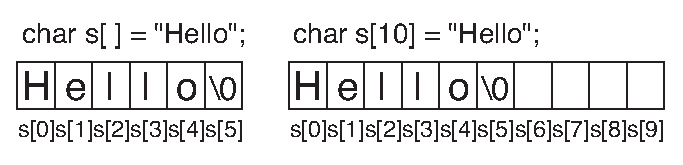
\includegraphics{hello.eps}}
\end{center}
\end{figure}

%===============================================================================
\subsection{標準入力(1) : {\tt gets}関数}
%-------------------------------------------------------------------------------
例\ref{ex:gets}を作成しコンパイルしてみよう(コンパイラによっては、「\verb|gets| は危険だ」と警告が出るかもしれないが、実行ファイルはちゃんとできているはずである)。これを実行すると、\verb|Input:| と表示され入力を促される。ここで、\verb|uni|などと入力すると、\verb|uni|と表示されてプログラムが終了する。この場合、\verb|gets|という関数によって入力された文字列が \verb|str| にコピーされる。注意すべきことは、\verb|str| が \verb|str[20]| と宣言されているので入力すべき文字列は19文字以内に限られるということである。しかし実際には、ユーザーは20字以上入力することができる。その場合、はみ出た文字は用意された領域の外に書き込まれる。もしそこが、別の変数用に使われていたら? これはとても危険なことである。\verb|gets|を使う場合は注意が必要である。
%
\begin{reidai}\label{ex:gets}
\begin{verbatim}
#include <stdio.h>
int main() {
  char str[20];
  printf("Input: ");
  gets(str);
  printf("%s\n", str);
  return 0;
}
\end{verbatim}
\end{reidai}
%

\subsection{標準入力(2) : {\tt scanf}関数}
例\ref{ex:gets}ではたとえ数字(19桁以下)を入力してもそれは文字列として扱われるため、数字として足し算などに用いるためには \verb|atoi|などの関数を用いる必要がある。数字を入力してそのまま数字として扱う方法を例\ref{ex:scanf}に示す。この場合、\verb|scanf| という関数を用いている。(ソースコード中の \verb|&i| や \verb|&x| の \verb|&| は今は気にしなくて良い。)
%
\begin{reidai}\label{ex:scanf}
\begin{verbatim}
#include <stdio.h>
#include <string.h>
int main() {
  int i;
  double x;
  printf("Input(int): ");
  scanf("%d", &i);
  printf("%d\n", i);
  printf("Input(double): ");
  scanf("%lf", &x);
  printf("%lf\n", x);
  return 0;
}
\end{verbatim}
\end{reidai}
%

%===============================================================================
%\subsection{練習}
%-------------------------------------------------------------------------------
\begin{renshuu}\label{prob:4-1}
練習\ref{prob:2-2}で、標準入力から $n$ を決定し、その答えを表示するプログラムを書きなさい。
\end{renshuu}

%*******************************************************************************
\section{ポインタ}
%===============================================================================
ポインタの習得はC言語の習得の中でひとつの大きな壁である。はじめは訳がわからないかもしれないが、C言語の基本的な部分の1つなので、いろいろな例に触れて慣れてほしい。慣れが一番である。

%===============================================================================
\subsection{とりあえず(1)}
%-------------------------------------------------------------------------------
例\ref{ex:pointer1}を作成し実行してみよう。上手くいけば、``{\tt q is 200 and *p is 200.}''と表示されるはずである。この例で出てくる \verb|p| がポインタである。\verb|int| 型のポインタを宣言するには、
%
\begin{quote}
\begin{verbatim}
int *p;
\end{verbatim}
\end{quote}
%
のように\verb|*|をつけて宣言する。そして、\verb|p| が \verb|int| のポインタで、\verb|*p| が \verb|int| になる。人によっては、
%
\begin{quote}
\begin{verbatim}
int* p;
\end{verbatim}
\end{quote}
%
と宣言したほうがイメージしやすいかもしれない。つまり、\verb|p| は \verb|int*| 型(\verb|int| のポインタ)ということである。(しかし、2個以上のポインタを宣言するためには、\verb|int *p, *q;| としなければならない。\verb|int* p, q;| とすると意味が変わってしまう。)

\verb|p| という \verb|int| 型のポインタは、\verb|int| 型の変数のアドレスを指し示す働きをする。アドレスとは大雑把にいえば、次のようなものである。例\ref{ex:pointer1}の \verb|int q; q = 200;| の \verb|q| に格納されている200はコンピュータのメモリーのどこかに電気的に存在するはずである。その物の場所を示すものがアドレスである。メモリー上の住所である。したがって、例\ref{ex:pointer1}では \verb|p = &q;| の文によって、\verb|p| は \verb|q| を指し示すことになる。(\verb|&q| は \verb|q| のアドレスを表す。) これにより、\verb|q| は \verb|q| 自身だけでなく、\verb|p| というポインタによってもアクセスすることができるようになる。
%
\begin{reidai}\label{ex:pointer1}
\begin{verbatim}
#include <stdio.h>
int main() {
  int *p;
  int q;
  q = 200;
  p = &q;
  printf("q is %d and *p is %d.\n", q, *p);
  return 0;
}
\end{verbatim}
\end{reidai}
%
\begin{figure}[H]
\begin{center}
\resizebox{0.60\textwidth}{!}{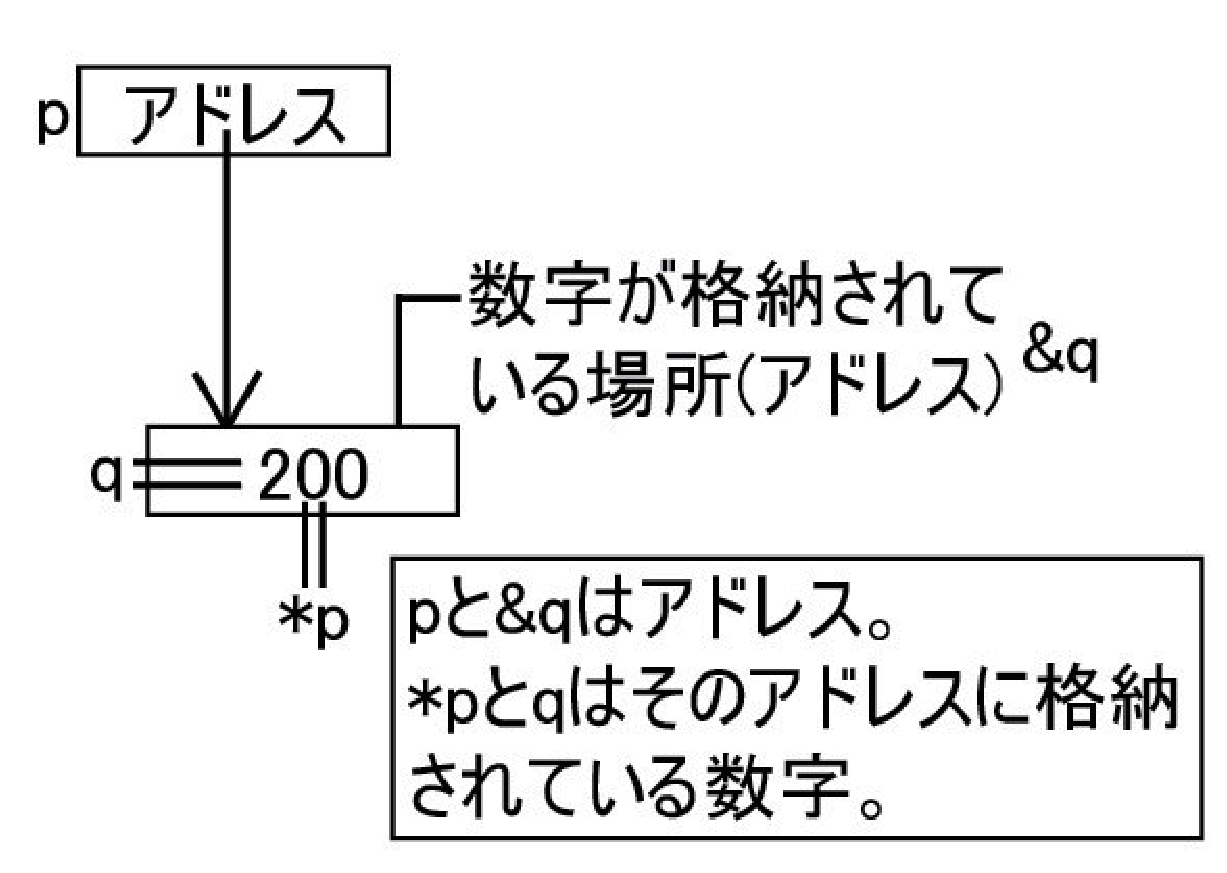
\includegraphics{pointer.eps}}
\end{center}
\end{figure}

%===============================================================================
\subsection{とりあえず(2)}
%-------------------------------------------------------------------------------
では、もう1つ例を示そう。例\ref{ex:pointer2}では、\verb|p = &q;| により \verb|p| というポインタで \verb|q| にアクセスできる。ここでは、\verb|q| に値を代入するかわりに、\verb|*p|を用いて値を代入している。\verb|p|はポインタで、\verb|*p| は \verb|p| が示しているアドレスにある値そのものである。
実行結果は、``{\tt q is 300 and *p is 300.}''となる。
%
\begin{reidai}\label{ex:pointer2}
\begin{verbatim}
#include <stdio.h>
int main() {
  int *p;
  int q;
  p = &q;
  *p = 300;
  printf("q is %d and *p is %d.\n", q, *p);
  return 0;
}
\end{verbatim}
\end{reidai} \noindent
%
記号{\tt *}, {\tt \&}などの意味と役割をもう一度復習しておこう。
%
\begin{quote}
\begin{verbatim}
int *p;
int q;
\end{verbatim}
\end{quote}
%
の時、
%
\begin{table}[H]
\begin{center}
\begin{tabular}{ll}
  \verb|p|  &ポインタ (つまりどこかのアドレス)\\
  \verb|*p| &実体\\
  \verb|q|  &実体\\
  \verb|&q| &\verb|q| のアドレス
\end{tabular}
\end{center}
\end{table} \noindent
%
注意すべきことは、例\ref{ex:pointer1}や例\ref{ex:pointer2}で \verb|p = &q;| がない場合は \verb|p| がどこを指しているか未定義であるということだ。したがって、\verb|*p = 300;| や \verb|printf| 内で \verb|*p| を表示させるのは危険である。何が起こるか分からない。

この節では、静的に宣言された変数を指すためにポインタを用いてきたが、より高度な使い方については\ref{sec:clang:malloc}節で紹介する。

%===============================================================================
\subsection{ポインタと配列}
\label{sec:C:pointer-array}
%-------------------------------------------------------------------------------
ポインタと配列には密接な関係がある。
%
\begin{quote}
\begin{verbatim}
int array[10];
\end{verbatim}
\end{quote}
%
と宣言した場合、\verb|array[0]| や \verb|array[5]| などで配列の要素にアクセスすることができた。実は、\verb|array| だけでも意味を持つ。\verb|array| は配列型 (\verb|int[10]| 型) の変数で、プログラムコード中に登場した時は、大抵の状況では、自動的に ``配列の先頭要素のアドレス''に暗黙的に変換されて解釈される。つまり、\verb|array| は \verb|array[0]| へのポインタとして解釈され、\verb|*array| は \verb|array[0]|を意味する。さらに、ポインタに整数を足すとその数だけ先の要素を指すようになる。例えば\verb|array+2|は\verb|array[2]| へのポインタであり、\verb|*(array+2)| は \verb|array[2]|と等価である。

では、例\ref{ex:pointer-array}を見てみよう。\verb|strlen| という関数は string.h 内で宣言されている文字列の長さを返す関数である。最初の \verb|for| 文は文字型の配列 \verb|str| の中身を順番に書き出している。次の \verb|for| 文がポイントである。まず、文字型のポインタ \verb|p| に文字型の配列 \verb|str| の先頭ポインタ \verb|str| を代入している。そして、文字型の実体である \verb|*p| が \verb|\0| でない場合はその \verb|*p| を表示し、ポインタ \verb|p| の指す部分をひとつ進めている。これを \verb|*p| が \verb|\0| になるまで繰り返すことで、最初の \verb|for| 文と同じ結果を表示している。
%
\begin{reidai}\label{ex:pointer-array}
\begin{verbatim}
#include <stdio.h>
#include <string.h>
int main() {
  char str[] = "ABCDE";
  int num = strlen(str);
  int i;
  for (i = 0; i < num; ++i) {
    printf("%c", str[i]);
  }
  printf("\n");
  char *p;
  for (p = str; *p != '\0'; ++p) {
    printf("%c", *p);
  }
  printf("\n");
  return 0;
}
\end{verbatim}
\end{reidai}
%

%===============================================================================
%\subsection{練習}
%-------------------------------------------------------------------------------
\begin{renshuu}\label{prob:5-1}
次のプログラムの \verb|printf| の部分を配列ではなく、ポインタを使ったものに書き換えなさい。(\verb|array| を使っても、あるいは、\verb|int *p;| を加えてもよい。)

\begin{quote}
\begin{verbatim}
#include <stdio.h>
int main() {
  int i;
  int array[10];
  for (i = 0; i < 10; ++i) {
    array[i] = i*i;
  }
  for (i = 0; i < 10; ++i) {
    printf("array[%d] = %d\n", i, array[i]);
  }
  return 0;
}
\end{verbatim}
\end{quote}
\end{renshuu}

%*******************************************************************************
\section{関数}
\label{sec:C:function}

%===============================================================================
\ref{sec:C:basic}節でC言語の基本構造を説明したが、\verb|main(){...}| だけでプログラムを書くことはほとんどない。大きなプログラムになればなるほど関数化を行い、役割分担をはっきりさせるのがよい。

%===============================================================================
\subsection{あまり良くない例}
%-------------------------------------------------------------------------------
例\ref{ex:non-function}は円の面積の計算するために直接その公式を書いている。しかし、何度も何度も円の面積を計算したいとき、半径を入力すれば面積が返ってくるような関数があれば非常に便利である。
%
\begin{reidai}\label{ex:non-function}
\begin{verbatim}
#include <math.h>
#include <stdio.h>
int main() {
  double radius = 2.0;
  double area = radius * radius * M_PI;
  printf("Radius: %lf, Area: %lf\n", radius, area);
  return 0;
}
\end{verbatim}
\end{reidai}
%

%===============================================================================
\subsection{関数化}
%-------------------------------------------------------------------------------
では、例\ref{ex:non-function}を例\ref{ex:function1}のように変更してみよう。このような小さなプログラムでは関数化の効力は乏しいが、大きくなればなるほど、また複雑になればなるほど、その効力は絶大になる。例\ref{ex:function1}では、\verb|circle_area| という関数が定義されている。この関数は、double型の値を引数として受け取り、面積を計算してその値を戻り値にしている。関数は使う前に宣言する必要がある。したがって、\verb|circle_area| 関数を \verb|main| の後や他のファイルに書く場合は、例\ref{ex:function2}のように使う前に宣言だけ行っておく必要がある。
%
\begin{reidai}\label{ex:function1}
\begin{verbatim}
#include <math.h>
#include <stdio.h>
double circle_area(double r) {
  return r*r*M_PI;
}

int main() {
  double radius = 2.0;
  double area = circle_area(radius);
  printf("Radius: %lf, Area: %lf\n", radius, area);
  return 0;
}
\end{verbatim}
\end{reidai}
%
\begin{reidai}\label{ex:function2}
\begin{verbatim}
#include <math.h>
#include <stdio.h>
double circle_area(double);

int main() {
  double radius = 2.0;
  double area = circle_area(radius);
  printf("Radius: %lf, Area: %lf\n", radius, area);
  return 0;
} 

double circle_area(double r) {
  return r*r*M_PI;
}
\end{verbatim}
\end{reidai}
%

%===============================================================================
\subsection{ポインタを引数にする関数}
%-------------------------------------------------------------------------------
例\ref{ex:function1}では関数の返り値が面積の1つだけであった。しかし、例えば割り算で商と余りを返したい場合、例\ref{ex:function1}のような関数ではうまく実現できない。なぜなら、戻り値は1個しか指定できないからである。これを解決するには、ポインタを引数とする関数を作る必要がある。答えを入れる箱をあらかじめ準備しておき、それを関数の引数にポインタとして渡し、関数内でそこに答えを入れてもらって、関数の外で受け取るという方法を用いる。重要な点は、ポインタでなければ関数内で代入した値を関数の外で使うことはできないということである。

例\ref{ex:function-pointer}では、まず{\tt main}で答えを入れてもらうための \verb|shou| と \verb|amari| という箱(変数)を準備している。次に、そのポインタ(アドレス)を関数\verb|division|に渡している。そして、\verb|division|内で答えを代入してもらい、関数の外で\verb|printf|を用いて答えを表示している。\verb|division| という関数の先頭にある\verb|void|という型は(返り値の形では)何も返さないことを示すためのものである。
%
\begin{reidai}\label{ex:function-pointer}
\begin{verbatim}
#include <stdio.h>
void division(int divident, int divisor, int *quotient, int *residual) {
  *quotient = divident / divisor;
  *residual = divident % divisor;
}

int main() {
  int josuu = 3;
  int hi_josuu = 13;
  int shou, amari;
  division(hi_josuu, josuu, &shou, &amari);
  printf("%d / %d = %d ... %d\n", hi_josuu, josuu, shou, amari);
  return 0;
}
\end{verbatim}
\end{reidai} \noindent
%
ポインタを使う理由がはっきりと分からない場合は、例\ref{ex:function-non-pointer}を作って実行してみてほしい。間違った答えが表示されるだろう。なぜなら、この場合 \verb|division| という関数では、\verb|quotient|と\verb|residual|という二つの一時変数が生成され、それらに計算結果が代入されるからである。それらの一時変数は関数の処理が終了すると同時に破棄され、値は \verb|main| の中の \verb|shou| と \verb|amari| には引き継がれない。関数に外部から値を渡すだけであれば、例\ref{ex:function-non-pointer}のような引数の宣言方法で良い(「値渡し」とよぶ)が、内での計算結果を関数の外で使いたい場合は、ポインタを使って変数のアドレスを渡す(「ポインタ渡し」とよぶ)必要がある。
%
\begin{reidai}\label{ex:function-non-pointer}
\begin{verbatim}
#include <stdio.h>
void division(int divident, int divisor, int quotient, int residual) {
  quotient = divident / divisor;
  residual = divident % divisor;
}

int main() {
  int josuu = 3;
  int hi_josuu = 13;
  int shou, amari;
  division(hi_josuu, josuu, shou, amari);
  printf("%d / %d = %d ... %d\n", hi_josuu, josuu, shou, amari);
  return 0;
}
\end{verbatim}
\end{reidai}
%

\subsection {Fortranの関数や手続きの利用}

LAPACK\footnote{行列の対角化、連立一次方程式の求解など線形計算を行うライブラリ。ほぼ全ての計算機で利用可能である。}などの多くのライブラリがFortranで書かれている。これらと同等の機能を持つ関数をCやC++で作ることもできるが、既に存在するのであればそちらを使った方が便利である。ここでは、C言語の中からFortranの関数や手続きを呼ぶ方法を簡単に紹介する。

Fortranの関数や手続きの名前をC言語から呼ぶためには、その名前をすべて小文字にして、最後に\_ (下線)を付けなければならない。また、関数などの引数の型も適切に読み変える必要がある。例えば、
\begin{reidai}
\begin{verbatim}
      Real*8 CALC(I, X, Y)
      Interger*4 I
      Real*4 X
      Real*8 Y
\end{verbatim}
\end{reidai} \noindent
というFortranの関数が存在するとする。このときCでは次のように使う。
\begin{reidai}
\begin{verbatim}
extern double clac_(int*, float*, double*);

int main() {
  int i = 10;
  float x = 20.0;
  double y = 30.0;
  double ret = calc_(&i, &x, &y);
  retrun 0;
}
\end{verbatim}
\end{reidai} \noindent
全ての引数をポインタ渡しとしなければならないことに特に注意せよ。コンパイルはCとFortranで別々に行い、最後にリンクすればよい。

%*******************************************************************************
\section{構造体}
%===============================================================================
データ構造を取り扱うためには構造体を用いる。

%===============================================================================
%\subsection{とりあえず}
%-------------------------------------------------------------------------------
例\ref{ex:struct1}を見てほしい。個人のデータを取り扱うために \verb|personal_data| という1つの箱を準備している。これが構造体である。もし構造体を使わなければ、同じ内容のプログラムを実現するためには複数の配列を準備する必要が出てくる。これは見た目にも格好悪いし、拡張性も乏しく複雑になる。例\ref{ex:struct1}では、\verb|struct personal_data pdata;| で \verb|pdata| を構造体とし宣言している。少し分かりにくいかもしれないが、\verb|int n;|と比べてみると、\verb|int| と ``\verb|struct personal_data|''が同じ立場であって、\verb|int| と ``\verb|struct|''が同じ立場というわけではないことに注意してほしい。\verb|int| という型はあらかじめC言語で決められた型なのに対し、構造体は自分が好きなように使いやすいように決めた型だと考えても構わない。つまり、``\verb|struct personal_data|''型というものを自分で作ったと考えるのである。そうすれば、\verb|struct personal_data pdata;| という使い方も理解できるはずである。

構造体内の各データには、ドット演算子 (\verb|.|) を使ってアクセスする。また、年齢を文字列 \verb|buffer[16]| として受け取っているため、\verb|atoi| 関数を用いて数字に変換している。\verb|atoi| は文字列を整数に変換する関数である。詳しくはコマンドラインで \verb|man atoi| としてみよ。
%
\begin{reidai}\label{ex:struct1}
\begin{verbatim}
#include <stdio.h>
#include <stdlib.h>
struct personal_data {
  char family_name[16];
  char given_name[16];
  int age;
};

int main() {
  struct personal_data pdata;
  char buffer[16];
  printf("Input family name: ");
  gets(pdata.family_name);
  printf("Input given name: ");
  gets(pdata.given_name);
  printf("Input age: ");
  gets(buffer);
  pdata.age = atoi(buffer);
  printf("Family Name = %s\n", pdata.family_name);
  printf("Given  Name = %s\n", pdata.given_name);
  printf("Age         = %d\n", pdata.age);
  return 0;
}
\end{verbatim}
\end{reidai} \noindent
%
構造体を指すポインタの場合は、次の例\ref{ex:struct2}のように、アロー演算子 (\verb|->|) でその構造体の要素にアクセスすることができる。例題中の\verb|qdata->p[0]|は\verb|(*qdata).p[0]|と等価である。ちなみに、この例の構造体は粒子の質量と運動量を格納している。
%
\begin{reidai}\label{ex:struct2}
\begin{verbatim}
#include <stdio.h>
struct particle_data {
  double mass;
  double p[3]; /* Momentum */
};

int main() {
  struct particle_data pdata;
  struct particle_data *qdata;
  pdata.mass = 0.14;
  pdata.p[0] = 1.2;
  pdata.p[1] = 1.3;
  pdata.p[2] = 1.4;
  qdata = &pdata;
  printf("Mass = %lf\n", qdata->mass);
  printf("Momentum = (%lf, %lf, %lf)\n", qdata->p[0], qdata->p[1], qdata->p[2]);
  return 0;
}
\end{verbatim}
\end{reidai}
%
%===============================================================================
%\subsection{練習}
%-------------------------------------------------------------------------------
\begin{renshuu}\label{prob:7-1}
``月'', ``日'', ``1月1日からの日数(うるう年ではない)''を構成要素とする構造体を作って、``月'' と ``日''を標準入力から入力すれば、自動的に ``1月1日からの日数''の部分を埋め、最後にそれを表示して終了するプログラムを書きなさい。
\end{renshuu}

%*******************************************************************************
\section{ファイルの取り扱い}
%===============================================================================
ファイルから数字を読みこんだり、ファイルに結果を書き込んだりするプログラムを紹介する。ここで挙げた例だけでも基本的なことはできるはずである。より詳しく知りたい場合は参考書などを参照してほしい。

%===============================================================================
\subsection{ファイルから数字の読み込み}
%-------------------------------------------------------------------------------
例\ref{ex:file-read1}がファイルから数字を読み込むときの雛型となる。まず、\verb|FILE *fp;| でファイルを取り扱うための構造体を宣言する。\verb|char *filename|の部分でファイル名を宣言する。そして、\verb|fopen|でファイルを開く。(\verb|"r"| はread (読み取り専用)でファイルを開くことを示す。) \verb|if(fp==NULL){}| の部分はエラーが起こったときに処理され、プログラムを強制終了させる。\verb|fscanf|で順番にファイルに書かれている数字を\verb|double|型で読み取っている。\verb|fscanf|の使い方は、
%
\begin{quote}
\begin{verbatim}
fscanf(ファイル構造体のポインタ, "フォーマット", &変数1, &変数2, ......);
\end{verbatim}
\end{quote}
%
で、ファイル構造体のポインタ部分以外は \verb|scanf| と同じである。そして、最後に \verb|fclose(fp);| でファイルを閉じている。
%
\begin{reidai}\label{ex:file-read1}
\begin{verbatim}
#include <stdio.h>
#include <stdlib.h>
double product(double x1, double y1, double x2, double y2) {
  return x1*y1 + x2*y2;
}

int main() {
  FILE *fp;
  char *filename = "vectors.txt";
  double x1,y1,x2,y2,p;
  fp = fopen(filename, "r");
  if (fp == NULL) {
    printf("Can't open file %s\n", filename);
    exit( 1 );
  }
  /* read first line */
  fscanf(fp, "%lf %lf\n", &x1, &y1);
  /* read second line */
  fscanf(fp, "%lf %lf\n", &x2, &y2);
  fclose(fp);
  p = product(x1, y1, x2, y2);
  printf("Product of (%lf,%lf) and (%lf,%lf) is %lf\n", x1, y1, x2, y2, p);
  return 0;
}
\end{verbatim}
\end{reidai} \noindent
%
例\ref{ex:file-read1}を実行するためには、{\tt vectors.txt}というファイル名で以下のような内容の入力ファイルも作っておく必要がある。
%
\begin{quote}
\begin{verbatim}
 1.0    2.0
-1.5    3.5
\end{verbatim}
\end{quote}
%
例\ref{ex:file-read1}のデータを読み込む部分を、例\ref{ex:file-read2}のように \verb|while| を使って書き直してみよう。こちらの方がファイルに存在するデータを最後まで読み取るという点で、より汎用性が高い。\verb|fscanf|はデータの読み込みに失敗すると\verb|EOF|を返すので、\verb|EOF|が返ってくるまで読み込みを繰り返している。
%
\begin{reidai}\label{ex:file-read2}
\begin{verbatim}
#include <stdio.h>
#include <stdlib.h>
#define N_DATA 100
int main() {
  FILE *fp;
  char *filename = "vectors.txt";
  double x[N_DATA][2];
  int index = 0;
  fp = fopen(filename, "r");
  if (fp==NULL) {
    printf("Can't open file %s\n", filename);
    exit(1);
  }
  /* read data */
  while (fscanf(fp, "%lf %lf\n", &x[index][0], &x[index][1]) != EOF) {
    printf("Data %d : (%lf, %lf)\n", index, x[index][0],x[index][1]);
    ++index;
  }
  fclose(fp);
  return 0;
}
\end{verbatim}
\end{reidai}
%
%===============================================================================
\subsection{ファイルへの数字の書き出し}
%-------------------------------------------------------------------------------
例\ref{ex:file-write}がファイルへ数字を書き出すときの雛型である。ファイルを開くところまでは例\ref{ex:file-read1}とはほぼ同じで、違う点は \verb|fopen| の第2引数が \verb|"r"| ではなく \verb|"w"| (書きこみ)である点である。また、書き出すときには \verb|fprintf| という関数を使っている。\verb|fprintf| の使い方は、
\begin{quote}
\begin{verbatim}
fprintf(ファイル構造体のポインタ, "フォーマット", 変数1, 変数2, ......);
\end{verbatim}
\end{quote}
%
で、ファイル構造体のポインタ部分以外は \verb|printf| と同じである。最後に、\verb|fclose(fp);| でファイルを閉じる。
%
\begin{reidai}\label{ex:file-write}
\begin{verbatim}
#include <stdio.h>
#include <stdlib.h>
#include <math.h>
double circle_area(double r) {
  return r*r*M_PI;
}

int main() {
  FILE *fp;
  char *filename = "circle_area.txt";
  double radius;
  int i;
  fp = fopen(filename, "w");
  if (fp == NULL) {
    printf("Can't open file %s\n", filename);
    exit(1);
  }
  for(i = 1; i <= 10; ++i) {
    radius = i * 1.0;
    double area = circle_area(radius);
    fprintf(fp, "%lf -> %lf\n", radius, area);
  }
  fclose(fp);
  return 0;
}
\end{verbatim}
\end{reidai}
%

%*******************************************************************************
\section{その他の制御文}
%===============================================================================
 {\tt for}, {\tt while}以外の制御文の書式を紹介する。

%===============================================================================
\subsection{{\tt switch}-{\tt case}文}
%-------------------------------------------------------------------------------
1の場合にはAを、2の場合にはBを、3の場合にはCを、という風に条件分岐をしたい場合に、\verb|switch|-\verb|case|文を用いる。
%
\begin{reidai}\label{ex:case}
\begin{verbatim}
#include <stdio.h>
#include <string.h>
int main() {
  int i;
  printf("Input(int): ");
  scanf("%d", &i);
  printf("%d / 3 no amari ha ", i);
  switch (i%3) {
    case 1:
      printf("1 desu.\n");
      break;
    case 2:
      printf("2 desu.\n");
      break;
    default:
      printf("0 desu.\n");
  }
  return 0;
}
\end{verbatim}
\end{reidai} \noindent
%
\verb|i%3|の結果が1であれば、\verb|case 1:| 以下の部分から実行する。\verb|i%3|の結果が2であれば、\verb|case 2:| 以下の部分から実行する。\verb|i%3|の結果が1でも2でもない場合、つまり、0の場合は、\verb|default:| 以下の部分から実行する。もちろん、\verb|case 0:| を作っても構わない。注意としては、もし例\ref{ex:case}の \verb|switch|-\verb|case| 文中に \verb|break;| がないと、\verb|case 1:| の場合は \verb|case 2:| の部分も \verb|default:| の部分も実行してしまうことである。つまり、\verb|case 1:| 以下の部分から下の部分をすべて実行するというこである。したがって、\verb|case 2:| の直前で抜けるためには \verb|break;| が必要となる。実際に \verb|break;| を削除して試してみよう。この場合は常に \verb|...0 desu.| が表示されるはずである。\verb|switch|-\verb|case| 文を簡単にまとめると、次のようになる。
%
\begin{quote}
\begin{verbatim}
switch (X) {
  case A:  ブロック1
  case B:  ブロック2
  case C:  ブロック3
  default: ブロック4
}
\end{verbatim}
\end{quote}
%
\verb|X|が\verb|A|ならば、ブロック1以下すべてを実行する。\verb|X|が\verb|B|ならば、ブロック2以下をすべて実行する。\verb|X|が\verb|C|ならばブロック3以下をすべて実行する。\verb|X|が\verb|A|でも\verb|B|でも\verb|C|でもない場合は、ブロック4を実行する。

%===============================================================================
\subsection{{\tt do}-{\tt while}文}
%-------------------------------------------------------------------------------
\verb|while| 文と同様に、ある条件が満たされている場合に繰り返しを行うために \verb|do|-\verb|while| 文を使う。\verb|while| 文と違う点は、条件の判定する``タイミング''である。\verb|while| 文の場合は、まず条件を判定し、満足していれば\verb|while| 内を実行するが、\verb|do|-\verb|while| 文の場合は、まず\verb|do|-\verb|while| 内を実行してから条件を判定する。したがって、\verb|while| 文の場合は \verb|while| 内を1度も実行しない場合があるが、\verb|do|-\verb|while| 文の場合は必ず1度は \verb|do|-\verb|while| 内を実行する。
%
\begin{reidai}\label{ex:do-while}
\begin{verbatim}
#include <stdio.h>
int main() {
  int i = 100;
  int sum = 0;
  do {
    sum += i;
    --i;
  } while (i != 0);
  printf("sum of integers from 100 to 1 is %d\n", sum);
  return 0;
}
\end{verbatim}
\end{reidai} \noindent
%
例\ref{ex:do-while}のように、\verb|while()| の後の \verb|;| を忘れないこと。
\verb|do|-\verb|while| 文の基本的な動作は次のようになる。
%
\begin{quote}
\begin{verbatim}
do {
  ブロック
} while (A);
\end{verbatim}
\end{quote}
%
まずブロックを実行し、次にAをチェックして正しいならば、再びブロックを実行する。そして、再びAをチェックして正しいならば、ブロックを実行する。したがって、Aが最初から間違いであってもブロックは必ず一度は実行される。

%===============================================================================
\subsection{{\tt goto}文}
%-------------------------------------------------------------------------------
最近では\verb|goto|文はあまり好まれないが、\verb|for|文がたくさん入り組んである場合(ネストという)に、\verb|for|文全体を一気に抜けるときに必要になることがある。\verb|goto|文は無条件に指定された部分に飛んでそこから実行を続けるために使う。例\ref{ex:goto}は\verb|goto|文を使うには全く不適切な例だが、イメージをつかむための練習として使ってほしい。簡単に説明すると、\verb|while| 文は \verb|while (1)| のように使っているので無限に繰り返し続けるが、\verb|i==0| となった時点で \verb|goto| を使って強引に \verb|owari:| という部分まで飛んでそこから実行を続ける。
%
\begin{reidai}\label{ex:goto}
\begin{verbatim}
#include <stdio.h>
int main() {
  int i = 100;
  int sum = 0;
  while (1) {
    sum += i;
    --i;
    if (i == 0) {
      goto owari;
    }
  }
owari:
  printf("sum of integers from 100 to 1 %d\n", sum);
  return 0;
}
\end{verbatim}
\end{reidai} \noindent
%
\verb|goto|文の基本的な使い方は以下の通りである。
\begin{quote}
\begin{verbatim}
  goto A;
  ...
A:
  ブロック2
\end{verbatim}
\end{quote}
\verb|goto A|の部分に来ると、\verb|A:|までジャンプしてその後のブロック2を実行する。例\ref{ex:goto}の \verb|owari:| を \verb|return 0;| の後にはそのままでは書けないことに注意しよう。なぜなら、\verb|owari:| の後には必ず何か実行するものが必要だからである。上の基本的な使い方の部分でも書いてあるように、\verb|A:|の後にはブロック(正確には``文'')が必要である。したがって、どうしても \verb|return 0;| の後に \verb|owari:| を書きたい場合は、\verb|owari:;|とする。

%*******************************************************************************
\section{コマンドライン引数の受け渡し}
%===============================================================================
{\tt main}文には、\verb|int main()| 以外に、\verb|int main(int, char**)|, あるいは \verb|int main(int, char*[])| という書き方がある。これらの書式を利用すれば、実行時に引数を与えてそれを利用することができる。つまり、今までは
\begin{commandline2}
\prompt \underline{./a.out}
\end{commandline2} \noindent
であったが、これを利用すれば、
\begin{commandline2}
\prompt \underline{./a.out input.data output.data}
\end{commandline2} \noindent
のように、ファイル名や数値などをコマンドライン引数としてプログラムに渡すことができる。

%===============================================================================
\subsection{ポインタ配列}
%-------------------------------------------------------------------------------
新しい\verb|main|関数の説明の前に、引数の受け渡しに使われているポインタ配列に関して説明しておこう。ポインタ配列は、名前通り、ポインタを要素とする配列(\verb|char*[]|)である。配列はポインタを使ってアクセス可能なので、``ポインタのポインタ'' (\verb|char**|)と同様に使うことができる。
\begin{reidai}\label{ex:pointers-array}
\begin{verbatim}
#include <stdio.h>
int main() {
  int i;
  char *name0 = "Alice";
  char *name1 = "Bob";
  char *name2 = "Claire";
  char *name3 = "David";
  char *name[4];
  name[0] = name0;
  name[1] = name1;
  name[2] = name2;
  name[3] = name3; /* A */
  for (i = 0; i < 4; ++i) { /* B */
    printf("Name%d : %s\n", i, name[i]);
  }
  for (i = 0; i < 4; ++i) { /* C */
    printf("Name%d : %c, %s\n", i, **(name+i), *(name+i));
  }
  return 0;
}
\end{verbatim}
\end{reidai} \noindent
%
例\ref{ex:pointers-array}の結果は以下のようになる。
%
\begin{quote}
\begin{verbatim}
Name0 : Alice
Name1 : Bob
Name2 : Claire
Name3 : David
Name0 : A, Alice
Name1 : B, Bob
Name2 : C, Claire
Name3 : D, David
\end{verbatim}
\end{quote}
%
まず、\verb|name[0]| の型は \verb|char*| なので、\verb|name0| の値等を代入することができる。Aの時点で、\verb|name| というポインタ配列の各要素にアドレスの代入したことになる。つまり、
%
\begin{quote}
\begin{verbatim}
name[0] = "Alice"という文字列の先頭アドレス
name[1] = "Bob"という文字列の先頭アドレス
name[2] = "Claire"という文字列の先頭アドレス
name[3] = "David"という文字列の先頭アドレス
\end{verbatim}
\end{quote}
%
となっている。したがって、Bの \verb|for| 文では、\verb|printf| に文字列の先頭アドレスを渡すことで、名前を表示することができる。次に、Cの \verb|for| 文であるが、これは若干混乱を招くが、次が理解出来れば、何とかクリアできるだろう。
%
\begin{center}
\begin{tabular}{r@{ = }c@{ = }l}
\verb|name|   & 文字へのポインタのポインタ & \verb|char**| 型\\
\verb|*name|  & 文字へのポインタ           & \verb|char*| 型\\
\verb|**name| & 文字                       & \verb|char| 型 (※ 文字列ではなく文字)
\end{tabular}
\end{center}
\verb|printf| は \verb|%s| で文字列の先頭アドレス、つまり、\verb|char*| を受け取り、\verb|%c| で文字型そのもの、つまり、\verb|char| を受け取る。また、\verb|name+i| という書き方は、例えば、\verb|name+1| の場合なら、\verb|name| が \verb|name[0]| なので、\verb|name+1| は \verb|name[1]| である。

%===============================================================================
\subsection{新しい{\tt main}関数}
%-------------------------------------------------------------------------------
例\ref{ex:new-main}がコマンドライン引数を受け取ることのできる \verb|main|関数の例である。{\tt int main(int argc, char* argv[])}は、{\tt int main(int argc, char** argv)}と書いても同じである。好きなほうを使えばよい。
また、伝統的に \verb|argc| と \verb|argv| という名前を使っているが、他の変数名でも構わない。
\begin{reidai}\label{ex:new-main}
\begin{verbatim}
#include <stdio.h>
#include <stdlib.h>
int main(int argc, char* argv[]) {
  FILE *fp;
  char *InputFileName;
  char *OutputFileName;
  int counter = 0;
  double x,y;
  double sumX = 0.0, sumY = 0.0;
  if (argc != 3) { /* A */
    printf("Usage: sumXY InputFile OutputFile\n");
    exit(1);
  }
  InputFileName = argv[1];
  OutputFileName = argv[2];
  /* input */
  fp = fopen(InputFileName, "r");
  if (fp==NULL) {
    printf("Can't open file %s\n", InputFileName);
    exit(1);
  }
  /* read data */
  while(fscanf(fp, "%lf %lf\n", &x, &y) != EOF) {
    sumX += x;
    sumY += y;
    ++counter;
  }
  fclose(fp);
  /* output */
  fp = fopen(OutputFileName, "w");
  if (fp == NULL) {
    printf("Can't open file %s\n", OutputFileName);
    exit(1);
  }
  /* write results */
  fprintf(fp, "Number of Data = %d\n", counter);
  fprintf(fp, "X Sum = %lf\n", sumX);
  fprintf(fp, "Y Sum = %lf\n", sumY);
  fclose(fp);
  return 0;
}
\end{verbatim}
\end{reidai} \noindent
例\ref{ex:new-main}を\ref{ex:new-main}cという名前で保存し、次のようにコンパイルする。
\begin{commandline2}
\prompt \underline{gcc -o sumXY \ref{ex:new-main}c}
\end{commandline2} \noindent
\verb|sumXY|は例\ref{ex:new-main}のAの部分の\verb|printf|のメッセージに合わせてある。次のように実行してみよう。
\begin{commandline2}
\prompt \underline{./sumXY}\\
Usage: sumXY InputFile OutputFile
\end{commandline2} \noindent
{\tt InputFile}, {\tt OutputFile}の二つのコマンドライン引数が必要であるという警告が表示される。例\ref{ex:new-main}のAの部分を変更することで、警告メッセージは変更することができる。次のように実行しても同じメッセージが出力されるはずである。
\begin{commandline2}
\prompt \underline{./sumXY input.dat}
\end{commandline2} \noindent
\begin{commandline2}
\prompt \underline{./sumXY input.dat output.dat 10}
\end{commandline2} \noindent
一番目の例は引数が足りず、二番目の例は引数が多すぎる。例\ref{ex:new-main}では \verb|argc| が3以外ならエラーメッセージを表示するようにしてあるので、
\begin{commandline2}
\prompt \underline{./sumXY input.dat output.dat 10}
\end{commandline2} \noindent
は3個の引数だからエラーが出るのはおかしい、と考えるかもしれない。しかし、これは正しい動作である。なぜなら、引数としてプログラム名(\verb|./sumXY|)も1個と数えられるからである\footnote{{\tt argv[0]}を用いると、例\ref{ex:new-main}のAのエラーメッセージは {\tt printf("Usage: \%s InputFile OutputFile\textbackslash n", argv[0]);}と書くことができる。このようにしておくと、プログラム名をあらかじめソースコードに明示的に書き込む(「ハードコーディング」とよぶ)必要がなくなる。}。つまり、二番目の例では、{\tt argc}の値は4であり、{\tt argv}の中身は
\begin{quote}
\begin{verbatim}
argv[0] = "./sumXY"の先頭アドレス
argv[1] = "input.dat"の先頭アドレス
argv[2] = "output.dat"の先頭アドレス
argv[3] = "10"の先頭アドレス
\end{verbatim}
\end{quote}
となっている。

最後に、1行に2個の数字で10行程度書いた{\tt input.dat}を作成し、次のように実行してみよう。{\tt output.dat}に結果が書き込まれているはずである。
\begin{commandline2}
\prompt \underline{./sumXY input.dat output.dat}
\end{commandline2}

%
%*******************************************************************************
\section{動的な配列の確保: {\tt malloc}と{\tt free}}
\label{sec:clang:malloc}
%===============================================================================
これまで、ポインタはあらかじめ確保した領域に対してのみ使ってきた。しかし、実行時に、入力値あるいは計算結果を反映して、50個のデータを取り扱いたいときもあれば、100個のデータを取り扱いたいときもある。もちろん、配列を利用してあらかじめ十分な大きさの領域(いまの場合は100個以上の数)を確保しておけばよいかもしれないが、平均的に10個ぐらいしか利用しないのに、たまに100個の場合があるからといって常に100個分の領域を確保しておくことは、無駄のように思える。これを回避するために、動的に、つまり、実行時に領域を確保する手段がある。それが、\verb|malloc| ({\bf m}emory {\bf alloc}cationの略)である。

%===============================================================================
\subsection{{\tt malloc}の使い方}
%-------------------------------------------------------------------------------
例\ref{ex:malloc}に\verb|malloc|の使い方の雛型を示す\footnote{簡単のため、コマンドライン引数のチェックは行っていない。実際のプログラムでは、配列を確保する前に確保しようとしているサイズを確認すべきである。}。\verb|malloc|は領域が確保できた場合はその領域の先頭アドレスを返すが、領域が確保できなかった場合は\verb|NULL|を返す。\verb|NULL|の場合は、何らかのエラー処理を行う必要がある。例\ref{ex:malloc}では、プログラムを強制的に終了している。\verb|sizeof|関数は型の大きさ(バイト数)を調べる関数である。この場合は\verb|int|の大きさ(通常4)を調べている。\verb|double|を大きさを調べたい場合は\verb|sizeof(double)|のように使う。例\ref{ex:malloc}では、\verb|int| の領域を \verb|n_element| 個分確保したいので、\verb|sizeof(int)*n_element|を\verb|malloc|に与えている。
%
\begin{reidai}\label{ex:malloc}
\begin{verbatim}
#include <stdio.h>
#include <stdlib.h>
int main(int argc, char* argv[]) {
  int* array;
  int n_element = atoi(argv[1]);
  if ((array = malloc(sizeof(int)*n_element)) == NULL) {
    printf("Can't allocate memory.\n");
    exit(1);
  }
  int i;
  for (i = 0; i < n_element; ++i) {
    array[i] = i*i;
  }
  for (i = 0; i < n_element; ++i) {
    printf("array[%d] = %d\n", i, array[i]);
  }
  return 0;
}
\end{verbatim}
\end{reidai} \noindent
なお、コンパイル時に、{\tt malloc}の部分で``型の不整合'' という警告が出る場合は、つぎのように明示的に型を変換すればよい。
\begin{quote}
\begin{verbatim}
array = (int*)malloc(sizeof(int)*n_element)
\end{verbatim}
\end{quote}
これをキャスト(型変換)という。
%
%===============================================================================
\subsection{{\tt free}の使い方}
%-------------------------------------------------------------------------------
例\ref{ex:malloc}には(引数の数のチェック以外にも)適切でない部分がある。\verb|malloc|で確保した領域を解放していない点である。確保した領域を解放するためには、\verb|free|という関数を使う\footnote{例\ref{ex:malloc}のようにプログラムがすぐに終了してしまう場合には、{\tt free}は必要ないと主張する人がいるかもしれない。その主張も確かに間違っている訳ではないが、本当に必要なときに忘れないために普段から書く癖をつけるべきである。}。
具体的には、例\ref{ex:malloc}の \verb|return 0;| の前に
%
\begin{verbatim}
     free(array);
\end{verbatim}
%
と1行書けば良い。

次に、例\ref{ex:malloc}を若干変更し、\verb|free|が重要となる例を考えよう。
\begin{reidai}\label{ex:malloc-free}
\begin{verbatim}
#include <stdio.h>
#include <stdlib.h>
int main(int argc, char* argv[]) {
  int* array;
  int n_element = atoi(argv[1]);
  int i, j;
  for (j = 0; j < 3; ++j) {
    if ((array = malloc(sizeof(int)*n_element) == NULL){
      printf("Can't allocate memory.\n");
      exit(1);
    }
    for (i = 0; i < n_element; ++i) {
      switch (j) {
        case 0:
          array[i] = i;
          break;
        case 1:
          array[i] = i*i;
          break;
        default:
          array[i] = i*i*i;
      }
    }
    for (i = 0; i < n_element; ++i) {
      printf("array[%d] = %d\n", i, array[i]);
    }
    free(array);
  }
  return 0;
}
\end{verbatim}
\end{reidai} \noindent
もし仮に\verb|free| がない場合、\verb|j=1| のとき、\verb|malloc| に成功すると \verb|array| は新しく確保された領域の先頭アドレスを持つ。この時、\verb|j=0|で確保した領域はどうなったのだろうか? その領域は、このプログラム自身が確保した領域として、このプログラムが終了するまで解放されない。しかも、\verb|array| はすでに \verb|j=0| のときに確保した領域を忘れているので、このプログラムからもその領域に適切にアクセスすることはできない。つまり、\verb|j=0| のときの領域はこのプログラムが持っているが、使うことができない領域として存在し続けることになる\footnote{これを「メモリリーク」と呼ぶ}。これは非常に無駄なことである。これを回避するためにも、使わなくなった領域は \verb|free| することが重要である。もちろん、最近の計算機はメモリ(および、スワップ領域)をたくさん積んでいるので例\ref{ex:malloc-free}程度のプログラムなら\verb|free|がなくても平気で最後まで動くはずであるが、習慣として、\verb|malloc| した領域を使い終わったら必ず \verb|free| するのがよい。
%
%

\section{練習問題の解答例}
%===============================================================================
以下に練習問題の解答例を示す。さまざまなプログラムの書き方があるので、これらの解答例にこだわらないこと。全く分からない場合に参考にする程度が望ましい。
%
\begin{renshuu-answer}{prob:2-1}
\baselineskip=12pt
\begin{verbatim}
#include <stdio.h>
int main() {
  /* ax+b=0 */
  double a = 4.0;
  double b = 1.0;
  printf("ax+b=0\n");
  printf("  a = %lf\n", a);
  printf("  b = %lf\n\n", b);
  if (a == 0.) {
    if (b == 0.) {
      printf("  x = all\n");
    } else {
      printf("  x = nothing\n");
    }
  } else {
    printf("  x = %lf\n", -b/a);
  }
  return 0;
}
\end{verbatim}
\end{renshuu-answer}
%
\begin{renshuu-answer}{prob:2-2}
\baselineskip=12pt
\begin{verbatim}
#include <stdio.h>
#include <stdlib.h>
int main() {
  /* calculate "n!" */
  int n = 10;
  if (n < 1){
    printf("Can't calculate n!.\n");
    printf("n = %d\n",n);
    exit(1);
  }
  int ans = 1;
  int i;
  for (i = 1; i <= n; ++i) {
    ans *= i;
  }
  printf("%d! = %d\n",n,ans);
  return 0;
}
\end{verbatim}
\end{renshuu-answer}
%
\begin{renshuu-answer}{prob:2-2}
\baselineskip=12pt
\begin{verbatim}
#include <stdio.h>
#include <stdlib.h>
int main() {
  /* calculate "n!" */
  int n = 10;
  if (n < 1) {
    printf("Can't calculate n!.\n");
    printf("n = %d\n",n);
    exit(1);
  }
  int ans = 1;
  int i = 1;
  while (i <= n) {
    ans *= i;
    ++i;
  }
  printf("%d! = %d\n",n,ans);
  return 0;
}
\end{verbatim}
\end{renshuu-answer}
%
\begin{renshuu-answer}{prob:2-3}
\baselineskip=12pt
\begin{verbatim}
#include <stdio.h>
int main() {
  /* n madeno sosuu. */
  int n = 100;
  printf("%d madeno sosuu = ", n);
  int ans = 2;
  while (ans <= n) {
    int flag = 0;
    int i;
    for (i = 2; i < ans; ++i) {
      if (ans%i == 0) {
        break;
      } else if (i == ans - 1) {
        flag = 1;
      }
    }
    if (flag == 1) {
      printf("%d, ", ans);
    }
    ++ans;
  }
  printf("\n");
  return 0;
}
\end{verbatim}
\end{renshuu-answer}
%
\begin{renshuu-answer}{prob:3-1}
\baselineskip=12pt
\begin{verbatim}
#include <stdio.h>
int main() {
  int a[5];
  a[0] = 1.0;
  a[1] = 2.0;
  a[2] = 3.0;
  a[3] = 4.0;
  a[4] = 5.0;
  int i;
  for (i = 0; i < 5; ++i) {
    printf("Start: a[%d] = %d\n", i, a[i]);
  }
  int b[5];
  for (i = 0; i < 5; ++i) {
    b[i] = a[i];
    a[i] = 0;
    printf("End  : a[%d] = %d, b[%d] = %d\n", i, a[i], i, b[i]);
  }
  return 0;
}
\end{verbatim}
\end{renshuu-answer}
%
\begin{renshuu-answer}{prob:3-2}
\baselineskip=12pt
\begin{verbatim}
#include <stdio.h>
void seki(double a[2][2], double b[2][2], double c[2][2]) {
  c[0][0] = a[0][0]*b[0][0] + a[0][1]*b[1][0];
  c[0][1] = a[0][0]*b[0][1] + a[0][1]*b[1][1];
  c[1][0] = a[1][0]*b[0][0] + a[1][1]*b[1][0];
  c[1][1] = a[1][0]*b[0][1] + a[1][1]*b[1][1];
}

int main() {
  double a[2][2], b[2][2];
  a[0][0] = 1.0;
  a[0][1] = 2.0;
  a[1][0] = 3.0;
  a[1][1] = 4.0;
  b[0][0] = -1.0;
  b[0][1] = -2.0;
  b[1][0] = -3.0;
  b[1][1] = -4.0;
  int i, j;
  for (i = 0; i < 2; ++i) {
    for (j = 0; j < 2; ++j) {
      printf("a[%d][%d] = %lf, b[%d][%d] = %lf\n",
             i, j, a[i][j], i, j, b[i][j]);
    }
  }
  double c[2][2];
  seki(a, b, c);
  for (i = 0; i < 2; ++i) {
    for (j = 0; j < 2; ++j) {
      printf("(a x b)[%d][%d] = %lf\n", i, j, c[i][j]);
    }
  }
  return 0;
}
\end{verbatim}
\end{renshuu-answer}
%
\begin{renshuu-answer}{prob:4-1}
\baselineskip=12pt
\begin{verbatim}
#include <stdio.h>
#include <string.h>
#include <stdlib.h>
int main() {
  /* calculate "n!" */
  int n;
  printf("Input(int): ");
  scanf("%d",&n);
  if (n < 1) {
    printf("Can't calculate n!.\n");
    printf("n = %d\n", n);
    exit(1);
  }
  int ans = 1;
  int i;
  for (i = 1; i <= n; ++i) {
    ans *= i;
  }
  printf("%d! = %d\n", n, ans);
  return 0;
}
\end{verbatim}
\end{renshuu-answer}
%
\begin{renshuu-answer}{prob:5-1}
\baselineskip=12pt
\begin{verbatim}
#include <stdio.h>
int main() {
  int array[10];
  int *p;
  int i;
  for (i = 0; i < 10; ++i) {
    array[i] = i*i;
  }
  for (i = 0; i < 10; ++i) {
    printf("array[%d] = %d\n", i, *(array+i));
  }
  for (i = 0; i < 10; ++i) {
    p = &(array[i]);
    printf("array[%d] = %d\n", i, *p);
  }
  return 0;
}
\end{verbatim}
\end{renshuu-answer}
%
\begin{renshuu-answer}{prob:7-1}
\baselineskip=12pt
\begin{verbatim}
#include <stdio.h>
struct date {
  unsigned int day, month;
  unsigned int days;
};

int main() {
  unsigned int nMonth[12] = { 31, 28, 31, 30, 31, 30,
                              31, 31, 30, 31, 30, 31 };
  struct date inputDay;
  printf("Input(month & day) :\n");
  printf("             month :");
  scanf("%d", &(inputDay.month));
  printf("             day   :");
  scanf("%d", &(inputDay.day));
  inputDay.days = 0;
  int i;
  for (i = 1; i < inputDay.month; ++i) {
    inputDay.days += nMonth[i-1];
  }
  inputDay.days += inputDay.day;
  printf("%d/%d = %d days from 1/1\n", inputDay.month,
         inputDay.day, inputDay.days);
  return 0;
}
\end{verbatim}
\end{renshuu-answer}
%


\chapter{\LaTeX 入門}
\chapter{\LaTeX 入門}

\noindent
\LaTeX はL. Lamportの開発した文書清書ソフトウェアである。もともとは、D. Knuthの開発した \TeX と呼ばれるソフトウェアで、これを使いやすく拡張したものである。近年では、数式関連の機能をさらに拡張したAMS\LaTeX も広く使われている。\LaTeX はワードプロセッサのようなソフトウェアではない。画面を見ながら文書を整形しその見たままの姿が印刷結果となるのがワードプロセッサである。例えば代表的なワードプロセッサであるMicrosoft Office Wordでは、段落や2段組、箇条書などの編集を画面を見ながら行えて、そして画面のイメージがほぼそのまま印刷される。一方、\LaTeX では見たままが印刷結果となるわけではないが、ワードプロセッサに匹敵する強力な清書機能を持っている。とくに、\LaTeX は数式の清書能力に長けている。

\section{\LaTeX の実行}
\label{sec:latex:intro}

では、さっそく例を見てみよう。適当なエディタで
\begin{reidai}
\label{reidai:latex:ex}
\begin{verbatim}
\documentclass{jarticle}
\begin{document}
$a$のまわりのテイラー展開
\begin{equation}
f(x) = \sum_{n=0}^{\infty} \frac{f^{(n)}(a)}{n!}(x-a)^n
\end{equation}
\end{document}
\end{verbatim}
\end{reidai} \noindent
と入力してみよう。このファイルを \texttt{ex.tex} という名前で保存する。このファイルを \LaTeX で処理するには、\texttt{platex}コマンド\footnote{日本語版\LaTeX 。英語のみを含む文書を処理する場合には、\texttt{latex}コマンドを使えばよい。}と\texttt{dvipdfmx}コマンドを実行する。
\begin{commandline2}
\prompt \underline{platex ex.tex}\\
\prompt \underline{dvipdfmx ex.dvi}
\end{commandline2} \noindent
一行目の \texttt{platex}コマンドでDVIファイル(\texttt{ex.dvi})が生成される。DVIは{\textbf{d}e\textbf{v}ice-\textbf{i}ndependent file format}の略で、最終的な出力形式(今の例ではPDF)に依存しない出力形式である。\texttt{dvipdfmx}コマンドは、このDVIファイルからPDF形式のファイルを生成する。これらのコマンドの実行後、\texttt{ex.pdf}というファイルができていれば成功である。では処理結果を見てみよう。macOSで作業している場合には、
\begin{commandline2}
\prompt \underline{open ex.pdf}
\end{commandline2} \noindent
Linuxで作業している場合には、
\begin{commandline2}
\prompt \underline{evince ex.pdf}
\end{commandline2} \noindent
でPDFファイルを開くことができる。結果は以下のようになっているはずである。
\renewcommand{\theequation}{1}
\begin{kekka}
\label{kekka:ex}
$a$のまわりのテイラー展開
\begin{equation}
 f(x) = \sum_{n=0}^{\infty} \frac{f^{(n)}(a)}{n!}(x-a)^n
\end{equation}
\vspace{0pt}
\end{kekka}

\paragraph{この章のまとめ}

\begin{itemize}
\item \LaTeX ファイルの拡張子は\texttt{.tex}である。
\item \LaTeX を使うには、\verb|platex| コマンドを実行する。
\item \texttt{platex}コマンドを実行すると、DVIファイル(拡張子は \texttt{.dvi})が生成される。
\item DVIファイルをPDF形式に変換するには、\verb|dvipdfmx| コマンドを実行する。
\item PDFファイルを見るには、``\verb|open PDFファイル名|'' (macOSの場合)、あるいは``\verb|evince PDFファイル名|'' (Linuxの場合)を実行する。
\end{itemize}

\section{\LaTeX に関する全体的なこと}
\label{sec:latex:global}

すでに例\ref{reidai:latex:ex}で見たとおり、\LaTeX のソースファイルには、本文以外の情報も書き込まれている。具体的には、
\begin{reidai}
\label{reidai:latex:template}
\begin{verbatim}
\documentclass{jarticle}
\usepackage[dvipdfmx]{graphicx}
\begin{document}

% ここに本文を書く

\end{document}
\end{verbatim}
\end{reidai} \noindent
のところがかならず書かなくてはならないところである。特に \verb|\begin{document}|より前の部分をプリアンブルと呼ぶ。以下の例題では、このかならず書かなくてはいけない部分を省略してあるので注意すること。

さて、 例\ref{reidai:latex:template}にはパーセント記号(\texttt{\%})で始まる行が書かれている。 \LaTeX では、\texttt{\%}で始まる行はコメントとみなされる。行の途中で\texttt{\%}が現われたときは、そこから行の最後までがコメントになる。コメントは\LaTeX の動作には影響を与えない。

文章はソースファイルの中にそのまま書けばよい。ソースファイルの途中で改行しても清書の結果には影響を与えない。また、空行を挟むとそこで改段落される。
\begin{reidai}
\begin{verbatim}
スーパーカミオカンデ実験の説明

スーパーカミオカンデは、世界最大の水チェレンコフ
宇宙素粒子観測装置です。1991年に建設が始まり、
5年間にわたる建設期間を経たのち、1996年4月より
観測を開始しました。
\end{verbatim}
\end{reidai} \noindent
この出力は、
\begin{kekka}
スーパーカミオカンデ実験の説明

スーパーカミオカンデは、世界最大の水チェレンコフ
宇宙素粒子観測装置です。1991年に建設が始まり、
5年間にわたる建設期間を経たのち、1996年4月より
観測を開始しました。
\end{kekka} \noindent
となる。出力は、もっとも美しく清書されるように、\LaTeX が自動的に改行を行なってくれる。逆にどうしても自分で改行させたいときは、\textbackslash \textbackslash をソースファイル中に書き込めばよい。
\begin{reidai}
\begin{verbatim}
東京大学物性研究所 \\ \\
秋葉原からつくばエクスプレスに乗り、
柏の葉キャンパス前で下車します。\\
運賃は670円です。\\
所要時間はおよそ30分です。
\end{verbatim}
\end{reidai} \noindent
結果は次のとおりである。
\begin{kekka}
東京大学物性研究所 \\ \\
秋葉原からつくばエクスプレスに乗り、
柏の葉キャンパス前で下車します。\\
運賃は670円です。\\
所要時間はおよそ30分です。
\end{kekka}

\paragraph{この節のまとめ}

\begin{itemize}
\item ソースファイルには必ず書かなくてはいけない部分がある。
\item \texttt{\%} から行の最後まではコメントである。
\item 文章はソースファイル中に直接書き込む。その際、改行は無視される。
\item 空行を挟むとそこで改段落される。
\item 強制改行をするには \textbackslash \textbackslash を使う。
\end{itemize}



\section{フォント}
\label{sec:latex:font}

印刷される文字を強調するために、文字を太くしたり(ボールド体)、ななめにしたり(斜体)することがある。印刷される文字の形状のことをフォントといい、その形状を変更することをフォントを変更するといいう。ちなみに、通常のフォントは立体と呼ばれる。

ボールド体はとくに強調したい言葉に使う。文章中でフォントを変更するには、
\begin{reidai}
\begin{verbatim}
東京駅から東京大学に向かうには、
\textbf{地下鉄丸ノ内線}を使うのが便利です。
\textbf{池袋}ゆきに乗り\textbf{本郷三丁目}駅で下車します。
\end{verbatim}
\end{reidai} \noindent
のように\verb|\textbf{文字}|命令を使う。結果は、
\begin{kekka}
東京駅から東京大学に向かうには、
\textbf{地下鉄丸ノ内線} を使うのが便利です。
\textbf{池袋}ゆきに乗り\textbf{本郷三丁目}駅で下車します。
\end{kekka} \noindent
となる。斜体は、変数などのパラメータを示したり、英単語を強調するのに用いる。
\begin{reidai}
\begin{verbatim}
\textbf{ls}コマンドに\textit{file}引数を渡すと
その\textit{file}に関する情報を表示します。
\end{verbatim}
\end{reidai}
\vspace*{-1.5em}
\begin{kekka}
\textbf{ls} コマンドに \textit{file} 引数を渡すと
その \textit{file} に関する情報を表示します。
\end{kekka} \noindent
タイプライタ体は計算機への入力、計算機からの出力、プログラムなどを示すのに使う。
\begin{reidai}
\begin{verbatim}
標準ライブラリ関数には、\texttt{sin()}や\texttt{cos()}、
\texttt{tan()} といった三角関数も用意されています。
\end{verbatim}
\end{reidai}
\vspace*{-1.5em}
\begin{kekka}
  標準ライブラリ関数には \texttt{sin()} や \texttt{cos()}、
  \texttt{tan()} といった
  三角関数も用意されています。
\end{kekka}

\paragraph{この節のまとめ}

\begin{itemize}
\item フォントの種類を変更するには \verb|\textbf{文字}| 、 \verb|\textit{文字}| 、\verb|\texttt{文字}| などを使う。
\end{itemize}


\section{論文のスタイル}
\label{sec:latex:style}

\LaTeX には論文を清書するのに便利な機能が備わっている。

\subsection{表題}
\label{sec:latex:title}

通常、論文の表題には、論文の題名、著者、著者の所属、提出日時、論文の要旨などを書く。
\begin{reidai}
\begin{verbatim}
\documentclass{jarticle}
\usepackage{graphicx}

% 表題、著者、所属、提出日時
\title{各種プログラミング言語に関する考察}
\author{物理太郎\\東京大学大学院理学系研究科物理学専攻}
\date{2019年4月8日}
\begin{document}

% 表題の表示
\maketitle

%%% ここに論文の本文を書く %%%

\end{document}
\end{verbatim}
\end{reidai} \noindent
レポート程度の簡単なものならば論文の要旨は不要であろう。結果は次のとおり。
\begin{kekka}
  \begin{center}
    {\Large 各種プログラミング言語に関する考察} \\[1.5em]
    物理太郎\\
    東京大学大学院理学系研究科物理学専攻 \\
    2019年4月8日
  \end{center}
\end{kekka}

\subsection{論文の構成}
\label{sec:latex:section}

通常、論文は内容にしたがって章分けされる。以下で \LaTeX で章を分ける例を示す。
\begin{reidai}
\begin{verbatim}
\section{C 言語}
C 言語は、
Brain Kernighan と Dennis Ritchie によって開発された
プログラミング言語である。
簡潔性と柔軟性の両方を備えたこの言語は、
さまざまな分野のソフトウェア開発に広く利用されている。
われわれが普段利用している UNIX オペレーティングシステムも
この C 言語を用いて記述されたものである。\\
\dots

\subsection{C 言語の歴史}
C 言語はベル研究所の Ritchie によって 1972 年頃開発された。
C 言語は Algol と呼ばれるプログラミング言語の流れを受け継ぐ言語で、
直接の母体は B 言語と呼ばれる言語である。\\
\dots

\subsection{C 言語の特徴}
この節では C 言語の特徴について述べよう。

\subsubsection{構造化プログラミング言語}
C 言語にはデータのまとまりを表す構造体と呼ばれるデータ型がある。
データを集合として扱う構造データ型は FORTRAN にはなかった。\\
\dots

\subsubsection{機械指向型プログラミング言語}
ひとつの C 言語の行なう命令は FORTRAN などに比べると簡潔であり
計算機に与えられる命令に近い。
これはプログラミング言語自体による副作用なしに
計算機を思い通りに直接操作できることを意味する。\\
\dots

\section{FORTRAN}
FORTRAN は FORmula TRANslator の名が示すとおり、
科学技術計算の能力に長けたプログラミング言語である。\\
\dots
\end{verbatim}
\end{reidai} \noindent
このように、章や節にタイトルを付けるには、\verb|\chapter{}|、\verb|\section{}|、\verb|\subsection{}|、\verb|\subsubsection{}|を使う。タイトルを\verb|{}|の中に書き、そのあとには本文となる文章を続ける。章や節の番号は\LaTeX が自動的に振ってくれる。
結果は次のようになる。
\begin{kekka}
  \begin{center}
    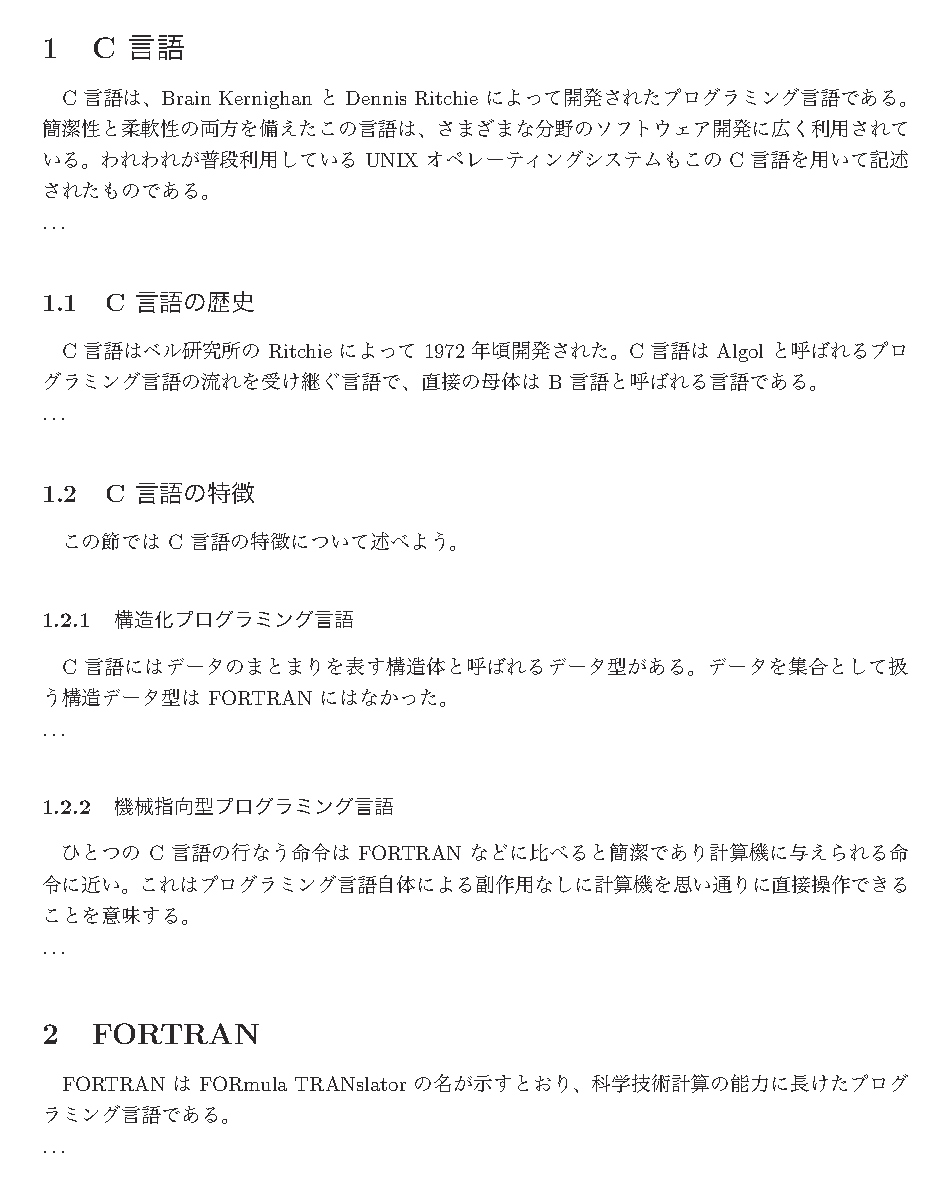
\includegraphics[bb=0 0 453 569, width=.9\textwidth]{section.pdf}
  \end{center}
\end{kekka}


\paragraph{この節のまとめ}

\begin{itemize}
\item 論文の表題は、\verb|\title{}| 、\verb|\author{}| 、\verb|\date{}| などで指定する。
\item 表題を出力するには、\verb|\maketile|を使う。
\item 章や節のタイトルを付けるには、\verb|\chapter{}|、\verb|\section{}|、 \verb|\subsection{}|、 \verb|\subsubsection{}| などを用いる。
\end{itemize}

\section{箇条書き}
\label{sec:latex:itemize}

論文の中では箇条書きを使うことは避けたほうがよいといわれている。特に、何かの処理の手順を説明するときは、箇条書きにするよりは言葉を使って説明するべきである。しかし、場合によっては箇条書きの方が説明が伝わりやすいこともある。単に項目を並列に並べたいときは箇条書きでもよいであろう。この節では箇条書きの方法を説明する。
箇条書きにしたいときは次のように書く。
\begin{reidai}
\begin{verbatim}
午後の紅茶(ミルクティー)の原材料名:
\begin{itemize}
  \item 牛乳
  \item 砂糖
  \item 加糖練乳
  \item 紅茶
  \item 香料
  \item 乳化剤
  \item ビタミン C
\end{itemize}
\end{verbatim}
\end{reidai} \noindent
このように、文章を\verb|\begin{itemize}|と\verb|\end{itemize}|とで囲むと、その領域は箇条書き環境になる。箇条書き環境の中では、\verb|\item|というコマンドを使うと新しい項目を始めることができる。
\begin{kekka}
  \def\labelitemisave{\labelitemi}
  \def\labelitemi{$\bullet$}
  午後の紅茶(ミルクティー)の原材料名:
  \begin{itemize}
  \item 牛乳
  \item 砂糖
  \item 加糖練乳
  \item 紅茶
  \item 香料
  \item 乳化剤
  \item ビタミン C
  \end{itemize}
  \def\labelitemi{\labelitemisave}
\end{kekka} \noindent
また、\texttt{itemize}の代わりに\texttt{enumerate}を使うと、各項目のラベルが1, 2, 3, $\cdots$のような番号となる。
\begin{reidai}
\begin{verbatim}
この講義の評価について該当するものに丸を付けて下さい。
\begin{enumerate}
\item 大変良かった。
\item まあまあ良かった。
\item 普通だった。
\item あまり良くなかった。
\item かなり良くなかった。
\end{enumerate}
\end{verbatim}
\end{reidai}
\vspace*{-1.5em}
\begin{kekka}
  この講義の評価について該当するものに丸を付けて下さい。
  \begin{enumerate}
  \item 大変良かった。
  \item まあまあ良かった。
  \item 普通だった。
  \item あまり良くなかった。
  \item かなり良くなかった。
  \end{enumerate}
\end{kekka}


\paragraph{この節のまとめ}

\begin{itemize}
\item \verb|\begin{itemize}| と \verb|\end{itemize}| で囲まれた部分は箇条書き環境になる。
\item \verb|\begin{enumerate}| と \verb|\end{enumerate}| で囲まれた部分は番号付き箇条書き環境になる。
\item 箇条書きの項目を始めるには\verb|\item|を使う。
\end{itemize}

\section{表の作成}
\label{sec:latex:table}

表を作成するには次に示す雛型を使えばよい。
\begin{reidai}
\begin{verbatim}
\begin{table}
  \begin{center}
    \caption{月刊誌の出版社と発売日}
    \begin{tabular}{|l|l|l|}
      \hline
      雑誌名 & 出版社 & 発売日 \\
      \hline \hline
      トランジスタ技術 & CQ出版 & 10 日 \\
      \hline
      UNIX Magazine & アスキー & 19 日 \\
      \hline
      SD ソフトウェアデザイン & 技術評論社 & 19 日 \\
      \hline
      アフタヌーン & 講談社 & 25 日 \\
      \hline
    \end{tabular}
  \end{center}
\end{table}
\end{verbatim}
\end{reidai}
\vspace*{-1.5em}
\begin{kekka}
  \begin{center}
    表1: 月刊誌の出版社と発売日 \\
    \begin{tabular}{|l|l|l|}
      \hline
      雑誌名 & 出版社 & 発売日 \\
      \hline \hline
      トランジスタ技術 & CQ出版 & 10 日 \\
      \hline
      UNIX Magazine & アスキー & 19 日 \\
      \hline
      SD ソフトウェアデザイン & 技術評論社 & 19 日 \\
      \hline
      アフタヌーン & 講談社 & 25 日 \\
      \hline
    \end{tabular}
  \end{center}
\end{kekka} \noindent
\verb|\hline| と書いたところには、横線が引かれる。\verb|\hline \hline|と2つ続けて書くと二重線になる。表の各行は、それぞれの要素の間を\texttt{\&}で区切り、最後に \texttt{\textbackslash \textbackslash} で改行して行が終わったことを\LaTeX に伝える。

この表は横の1行に3つの要素を持つ表である。各要素は表の1マスに左詰めで書かれている。このことは
\begin{quotation}
  \verb-\begin{tabular}{|l|l|l|}-
\end{quotation}
の\verb-{|l|l|l|}-によって表現されている。 \texttt{l} は左詰めを意味し、それを3つ並べることで、1行に3つの要素が入ることを表現している。左詰めの代わりに中央揃えがよければ\texttt{c}を、右詰めがよければ\texttt{r}を指定する。

それぞれの\texttt{l}の両隣の縦棒は、要素と要素の間を縦線で区切って印刷してほしいということを\LaTeX に伝えている。この縦棒を取ってしまうと、要素間の縦線が引かれなくなる。

表の表題は
\begin{quotation}
  \verb|\caption{月刊誌の出版社と発売日}|
\end{quotation}
のように \verb|\caption| の後の \verb|{}| の中に書く。
最後にもう1つ例を挙げておこう。
\begin{reidai}
\begin{verbatim}
\begin{table}
  \begin{center}
    \caption{代表的な粒子の質量}
    \begin{tabular}{|c|r|}
      \hline
      粒子 & 質量 (MeV/$c^2$) \\
      \hline \hline
      $e ^ \pm$ & 0.5110 \\
      \hline
      $\mu ^ \pm$ & 105.7 \\
      \hline
      $\pi ^ \pm$ & 139.6 \\
      \hline
      $\pi ^ 0$ & 135.0 \\
      \hline
      $J/\psi$ & 3097 \\
      \hline
      $B ^ 0$ & 5279 \\
      \hline
    \end{tabular}
  \end{center}
\end{table}
\end{verbatim}
\end{reidai}
\vspace*{-1.5em}
\begin{kekka}
  \begin{center}
    表1: 代表的な粒子の質量 \\
    \begin{tabular}{|c|r|}
      \hline
      粒子 & 質量 (MeV/$c^2$) \\
      \hline \hline
      $e ^ \pm$ & 0.5110 \\
      \hline
      $\mu ^ \pm$ & 105.7 \\
      \hline
      $\pi ^ \pm$ & 139.6 \\
      \hline
      $\pi ^ 0$ & 135.0 \\
      \hline
      $J/\psi$ & 3097 \\
      \hline
      $B ^ 0$ & 5279 \\
      \hline
    \end{tabular}
  \end{center}
\end{kekka}

\section{数式}
\label{sec:latex:math}

数式は、例\ref{reidai:latex:ex}で見たとおり、
\begin{reidai}
\begin{verbatim}
\begin{equation}
%%% ここに数式を書きます %%%
\end{equation}
\end{verbatim}
\end{reidai} \noindent
というスタイルで記述する。\verb|\begin{equation}|と\verb|\end{equation}|とで囲まれた範囲では、数式環境の中のみで有効な様々なコマンドが使える。また、数式の番号は自動的に振られる。

結果\ref{kekka:ex}で見たとおり、\verb|\begin{equation}|と\verb|\end{equation}|とで囲まれた領域の数式は、改まった行の中央に表示される。しかし、場合によっては
\addtocounter{reidai}{1}
\begin{kekka}
  \label{kekka:math}
  $x$ の関数 $y = ax ^ 2 + bx + c$ のうち
  $a \ne 0$ であるものを $x$ の 2 次関数といいます。
\end{kekka} \noindent
\addtocounter{reidai}{-1}
のように文章中にインラインで数式を書きたいこともあるだろう。そういう場合は、文章中に\texttt{\$}と\texttt{\$}で囲った数式を書けばよい。結果\ref{kekka:math}を与えるソースは、以下のとおりである。
\begin{reidai}
\begin{verbatim}
$x$の関数$y = ax ^ 2 + bx + c$のうち
$a \ne 0$ であるものを$x$の2次関数といいます。
\end{verbatim}
\end{reidai} \noindent
以降の例題中ではスペースの都合上、2つ以上の数式を並べて書いてある場合があるが、、実際には1つずつ\verb|\begin{equation}|と\verb|\end{equation}|とで囲むか、\texttt{\$}と\texttt{\$}とで囲まなくてならない。

\subsection{添え字}
\label{sec:latex:index}

上付き添え字は\texttt{\^}で、上付き添え字は\texttt{\_}で表現する。
\begin{reidai}
\begin{verbatim}
y = a x ^ 2 + b x + c
S_n = a_1 + a_2 + a_3 + \cdots + a_n
\end{verbatim}
\end{reidai}
\vspace*{-1.5em}
\begin{kekka}
  \begin{equation*}
    y = a x ^ 2 + b x + c
  \end{equation*}
  \begin{equation*}
    S_n = a_1 + a_2 + a_3 + \cdots + a_n
  \end{equation*}
  \vspace{0pt}
\end{kekka} \noindent
2文字以上からなる項を添え字にしたいときは、\verb|{}|で添え字を囲む。
\begin{reidai}
\label{reidai:latex:2let_index}
\begin{verbatim}
Tr\,A = A_{11} + A_{22} + A_{33} + \cdots + A_{ii} + \cdots + A_{nn}
\end{verbatim}
\end{reidai}
\vspace*{-1.5em}
\begin{kekka}
  \begin{equation*}
    Tr\,A = A_{11} + A_{22} + A_{33} + \cdots + A_{ii} + \cdots + A_{nn}
  \end{equation*}
  \vspace{0pt}
\end{kekka} \noindent
添え字に限らず、\LaTeX の数式コマンドを2文字以上の項に作用させるときはかならず項を\verb|{}|で囲む必要がある。逆に1文字だけの項を\verb|{}|で囲んでも特に問題はない。なお、例\ref{reidai:latex:2let_index}の中で`\verb|\,|'というコマンドが使われているが、これはスペースの微調整をしたいときに使用する。

\subsection{分数}
\label{sec:latex:frac}

分数は\texttt{\textbackslash frac\{\textrm{分子}\}\{\textrm{分母}\}}の
ように表現する。
\begin{reidai}
\begin{verbatim}
1 + \frac{1}{2} = \frac{3}{2}
1 + \frac{1}{1+\frac{1}{2}} = \frac{5}{3}
\end{verbatim}
\end{reidai}
\vspace*{-1.5em}
\begin{kekka}
  \begin{equation*}
    1 + \frac{1}{2} = \frac{3}{2}
  \end{equation*}
  \begin{equation*}
    1 + \frac{1}{1+\frac{1}{2}} = \frac{5}{3}
  \end{equation*}
\end{kekka}

\subsection{関数}
\label{sec:latex:func}

数学環境では文字はすべて変数と見なされるため、\verb|cos x| という入力は$cos x$と斜体で印刷される。これではあたかも$c$、$o$、$s$、$x$の積のようである。数学関数は正しくは立体で表示されなくてはならない。立体で印刷するためには、\verb|\cos x|と入力する。このように数学関数の多くはバックスラッシュ(\texttt{\textbackslash})に関数名をつなげると表現できる。
\begin{reidai}
\begin{verbatim}
\frac{d}{dx} \sin x = \cos x
\end{verbatim}
\end{reidai}
\vspace*{-1.5em}
\begin{kekka}
  \begin{equation*}
    \frac{d}{dx} \sin x = \cos x
  \end{equation*}
\end{kekka}
\noindent
表\ref{tab:func}に主な数学関数を示す。
\begin{table}[H]
  \begin{center}
    \caption{主な数学関数}
    \label{tab:func}
    \begin{tabular}{ccc}
      \verb|\cos| & \verb|\sin| & \verb|\tan| \\
      \verb|\cosh| & \verb|\sinh| & \verb|\tanh| \\
      \verb|\log| & \verb|\ln| & \verb|\exp| \\
      \verb|\lim| & & \\
    \end{tabular}
  \end{center}
\end{table}

\subsection{フォント}
\label{sec:latex:mathfont}

前節でも触れたが、\LaTeX は立体で印刷したい文字も斜体で印刷してしまうことがある。数式中でフォントを強制的に変更するときは前に説明した方法は使わない。数式中で立体の文字を印刷するには、\texttt{\textbackslash mathrm\{\textrm{文字}\}}と書く。
\begin{reidai}
\begin{verbatim}
\frac{\mathrm d}{\mathrm{d}x}\mathrm{e}^x = \mathrm{e}^x
\end{verbatim}
\end{reidai}
\noindent これにより、立体で表示されるべきところは正しく立体で印刷される。
\begin{kekka}
  \begin{equation*}
    \frac{\mathrm d}{\mathrm{d}x}\mathrm{e}^x = \mathrm{e}^x
  \end{equation*}
\end{kekka}

\subsection{積分・和・積}
\label{sec:latex:integration}

積分、和、積は以下のように表現する。
\begin{reidai}
\begin{verbatim}
\int _1 ^2 \frac{1}{x^2} \mathrm{d}x = \frac{1}{2}
\sum _{k=1} ^n k = \frac{n(n+1)}{2}
n! = \prod _{k=1} ^n k
\end{verbatim}
\end{reidai}
\vspace*{-1.5em}
\begin{kekka}
  \begin{equation*}
    \int _1 ^2 \frac{1}{x^2} \mathrm{d}x = \frac{1}{2}
  \end{equation*}
  \begin{equation*}
    \sum _{k=1} ^n k = \frac{n(n+1)}{2}
  \end{equation*}
  \begin{equation*}
    n! = \prod _{k=1} ^n k
  \end{equation*}
\end{kekka}

\subsection{根号・ベクトル・上線・チルダ・ハット・時間微分}
\label{sec:latex:root}

根号、ベクトル、上線の記号は以下のように表現する。
\begin{reidai}
\begin{verbatim}
\sqrt{x^2 + 2x + 1} = |x+1|
\vec{x} + \vec{y} = \vec{z}
\overrightarrow{OA} + \overrightarrow{AP} = \overrightarrow{OP}
\overline{x + \mathrm{i}y} = x - \mathrm{i}y
\end{verbatim}
\end{reidai}
\vspace*{-1.5em}
\begin{kekka}
  \begin{equation*}
    \sqrt{x^2 + 2x + 1} = |x+1|
  \end{equation*}
  \begin{equation*}
    \vec{x} + \vec{y} = \vec{z}
  \end{equation*}
  \begin{equation*}
    \overrightarrow{OA} + \overrightarrow{AP} = \overrightarrow{OP}
  \end{equation*}
  \begin{equation*}
    \overline{x + \mathrm{i}y} = x - \mathrm{i}y
  \end{equation*}
\end{kekka} \noindent
同様にチルダ、ハット(演算子)、時間微分などは以下のように表現する。
\begin{reidai}
\begin{verbatim}
\tilde{x}
\hat{r}
\dot{x}
\end{verbatim}
\end{reidai}
\vspace*{-1.5em}
\begin{kekka}
  \begin{equation*}
    \tilde{x}
  \end{equation*}
  \begin{equation*}
    \hat{r}
  \end{equation*}
  \begin{equation*}
    \dot{x}
  \end{equation*}
\end{kekka}

\subsection{ギリシャ文字}
\label{sec:latex:greek}

ギリシャ文字は文字を英語表記で綴り、前にバックスラッシュを付けると表示される。$\alpha$ は \verb|\alpha| と入力する。ギリシャ文字の大文字は、英語の綴りの最初の 1 文字を大文字にすると表示できる。 \verb|\Psi| と書けば $\Psi$ が印刷される。
\begin{table}[H]
  \begin{center}
    \caption{ギリシャ文字一覧}
    \label{tab:greek}
    \begin{tabular}{|lcc|lcc|lcc|}
      \hline
      コマンド & 小文字 & 大文字 & コマンド & 小文字 & 大文字 & コマンド & 小文字 & 大文字 \\
      \hline \hline
      \verb|\alpha| & $\alpha$ & -- & \verb|\iota| & $\iota$ & -- & \verb|\rho| & $\rho$ & -- \\
      \verb|\beta| & $\beta$ & -- & \verb|\kappa| & $\kappa$ & -- & \verb|\sigma| & $\sigma$ & $\Sigma$ \\
      \verb|\gamma| & $\gamma$ & $\Gamma$ & \verb|\lambda| & $\lambda$ & $\Lambda$ & \verb|\tau| & $\tau$ & -- \\
      \verb|\delta| & $\delta$ & $\Delta$ & \verb|\mu| & $\mu$ & -- & \verb|\upsilon| & $\upsilon$ & $\Upsilon$ \\
      \verb|\epsilon| & $\epsilon$ & -- & \verb|\nu| & $\nu$ & -- & \verb|\phi| & $\phi$ & $\Phi$ \\
      \verb|\zeta| & $\zeta$ & -- & \verb|\xi| & $\xi$ & $\Xi$ & \verb|\chi| & $\chi$ & -- \\
      \verb|\eta| & $\eta$ & -- & \verb|o| & $o$ & $O$ & \verb|\psi| & $\psi$ & $\Psi$ \\
      \verb|\theta| & $\theta$ & $\Theta$ & \verb|\pi| & $\pi$ & $\Pi$ & \verb|\omega| & $\omega$ & $\Omega$ \\
      \hline
    \end{tabular}
  \end{center}
\end{table} \noindent
-- となっている箇所は、通常のアルファベットの大文字で代用する。

\subsection{行列}
\label{sec:latex:matrix}

行列を書く方法は表の作成と似ている。
\begin{reidai}
\begin{verbatim}
\sigma_3 = (
\begin{array}{cc}
  1 & 0 \\
  0 & -1 \\
\end{array} )
\end{verbatim}
\end{reidai} \noindent
表のところで説明されている書き方のうち、\verb|\begin{tabular}| から\verb|\end{tabular}| までをまねして、 \texttt{tabular} を \texttt{array} に書き換える。行列の丸カッコは自動的には印刷されないので自分で書く\footnote{ちなみに、AMS\LaTeX では{\tt pmatrix}環境が用意されており、行列をより自然な形で記述できる。}。
\begin{kekka}
  \begin{equation*}
    \sigma_3 = (
    \begin{array}{cc}
      1 & 0 \\
      0 & -1 \\
    \end{array} )
  \end{equation*}
  \vspace{0pt}
\end{kekka} \noindent
しかし、これではカッコの大きさがあまり美しくない。カッコを括られている内容の高さに合わせて大きくするには、\verb|\left(| と \verb|\right)| を使う。
\begin{reidai}
\begin{verbatim}
\phi (x) = \sqrt{\frac{1}{2}} \left(
\begin{array}{c}
  0 \\
  v + h(x)
\end{array} \right)
\end{verbatim}
\end{reidai} \noindent
\vspace*{-1.5em}
\begin{kekka}
  \begin{equation}
    \phi (x) = \sqrt{\frac{1}{2}} \left(
      \begin{array}{c}
        0 \\
        v + h(x)
      \end{array} \right)
  \end{equation}
  \vspace{0pt}
\end{kekka} \noindent
\verb|\left(| と \verb|\right)| の組み合わせは、中に入るものが行列でなくても使える。また、丸カッコ以外にも使える。
\begin{reidai}
\begin{verbatim}
J_{\mu}^{NC}(\nu) =
\frac{1}{2}
\left[
\overline{u}_{\nu}\gamma_{\mu} \frac{1}{2} (1-\gamma^5)u_\nu
\right]
\end{verbatim}
\end{reidai}
\vspace*{-1.5em}
\begin{kekka}
  \begin{equation}
    J_{\mu}^{NC}(\nu) =
    \frac{1}{2}
    \left[
      \overline{u}_{\nu}\gamma_{\mu} \frac{1}{2} (1-\gamma^5)u_\nu
    \right]
  \end{equation}
  \vspace{0pt}
\end{kekka} \noindent
このようにカギカッコなどにも使える。

\subsection{特殊記号}
\label{sec:latex:symbol}

最後に \LaTeX で使える特殊記号を示しておく。
\begin{table}[H]
  \begin{center}
    \caption{主な特殊記号}
    \label{tab:symbol}
    \begin{tabular}{|lc|}
      \hline
      コマンド & 印刷結果 \\
      \hline \hline
      \verb|\ne| & $\ne$ \\
      \verb|\le| & $\le$ \\
      \verb|\ge| & $\ge$ \\
      \verb|\equiv| & $\equiv$ \\
      \verb|\pm| & $\pm$ \\
      \verb|\times| & $\times$ \\
      \verb|\infty| & $\infty$ \\
      \verb|\bullet| & $\bullet$ \\
      \verb|\prime| & $\prime$ \\
      \verb|\dagger| & $\dagger$ \\
      \verb|\partial| & $\partial$ \\
      \verb|\to| & $\to$ \\
      \verb|\nabla| & $\nabla$ \\
      \verb|\triangle| & $\triangle$ \\
      \hline
    \end{tabular}
  \end{center}
\end{table}

\paragraph{この節のまとめ}

\begin{itemize}
\item 数式を書くには、\verb|\begin{equation}|と\verb|\end{equation}|で囲む。
\item 文章中で数式を書くには \texttt{\$} と \texttt{\$} で囲む。
\item 添え字、分数、関数、積分記号などについては、それぞれにコマンドが用意されている。
\end{itemize}

\section{図の貼り込み}
\label{sec:latex:picture}

\LaTeX では、{\tt gnuplot}などで生成した(\ref{sec:unix:gnuplot})節)図のファイル(ポストスクリプト、PDFなど)を文章中に貼り込むことが可能である。

\subsection{PDFファイルの貼り込み}
\label{sec:latex:include_pdf}

図を貼り込むには以下の雛型を用いる。
\begin{reidai}
\begin{verbatim}
\begin{figure}
  \begin{center}
    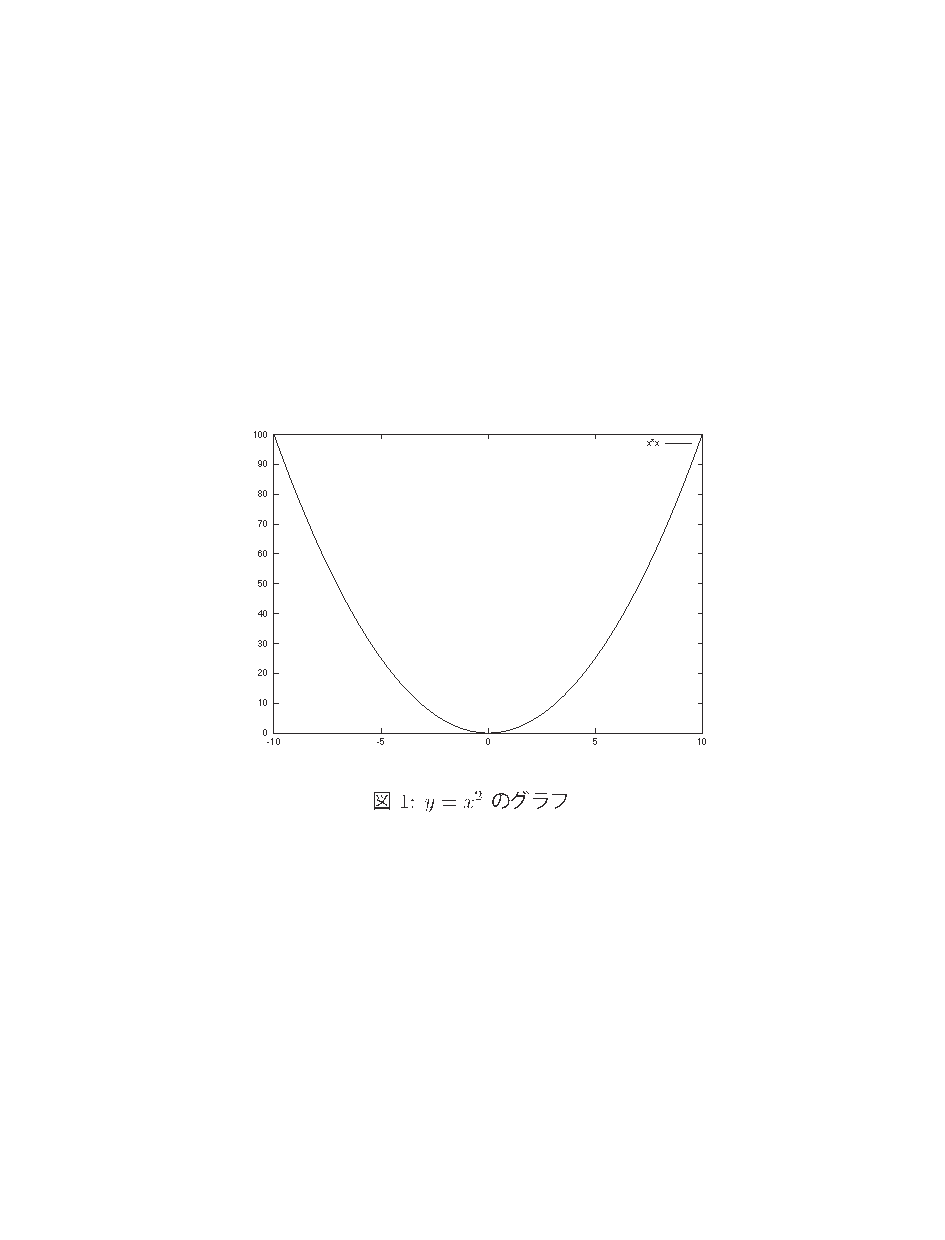
\includegraphics[width=8cm]{figure.pdf}
    \caption{$y = x^2$ のグラフ}
  \end{center}
\end{figure}
\end{verbatim}
\end{reidai}
\vspace*{-1.5em}
\begin{kekka}
  \begin{center}
    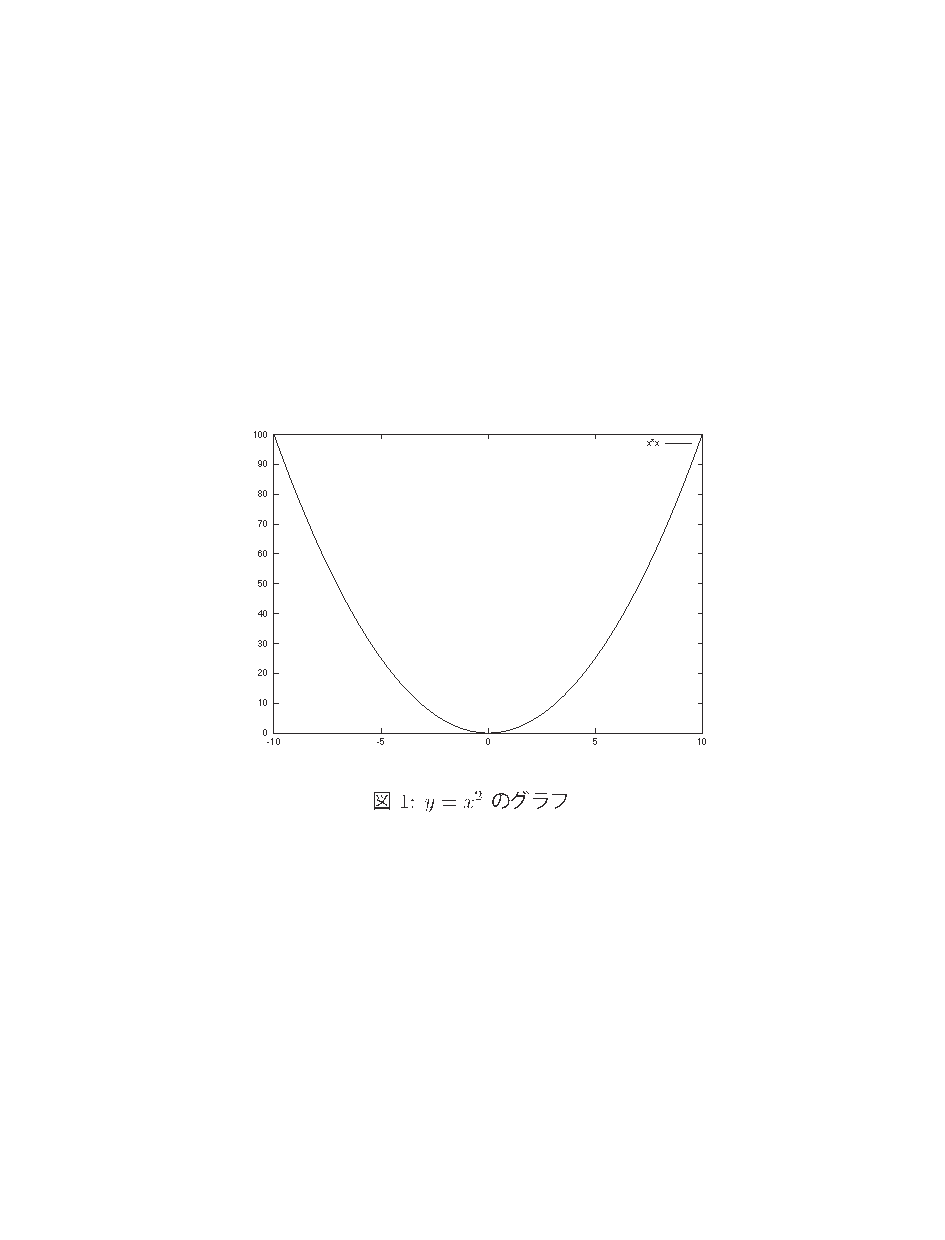
\includegraphics[width=8cm]{figure.pdf} \\
    図1: $y = x^2$ のグラフ
  \end{center}
\end{kekka} \noindent
注意すべきところは
\begin{quotation}
  \verb|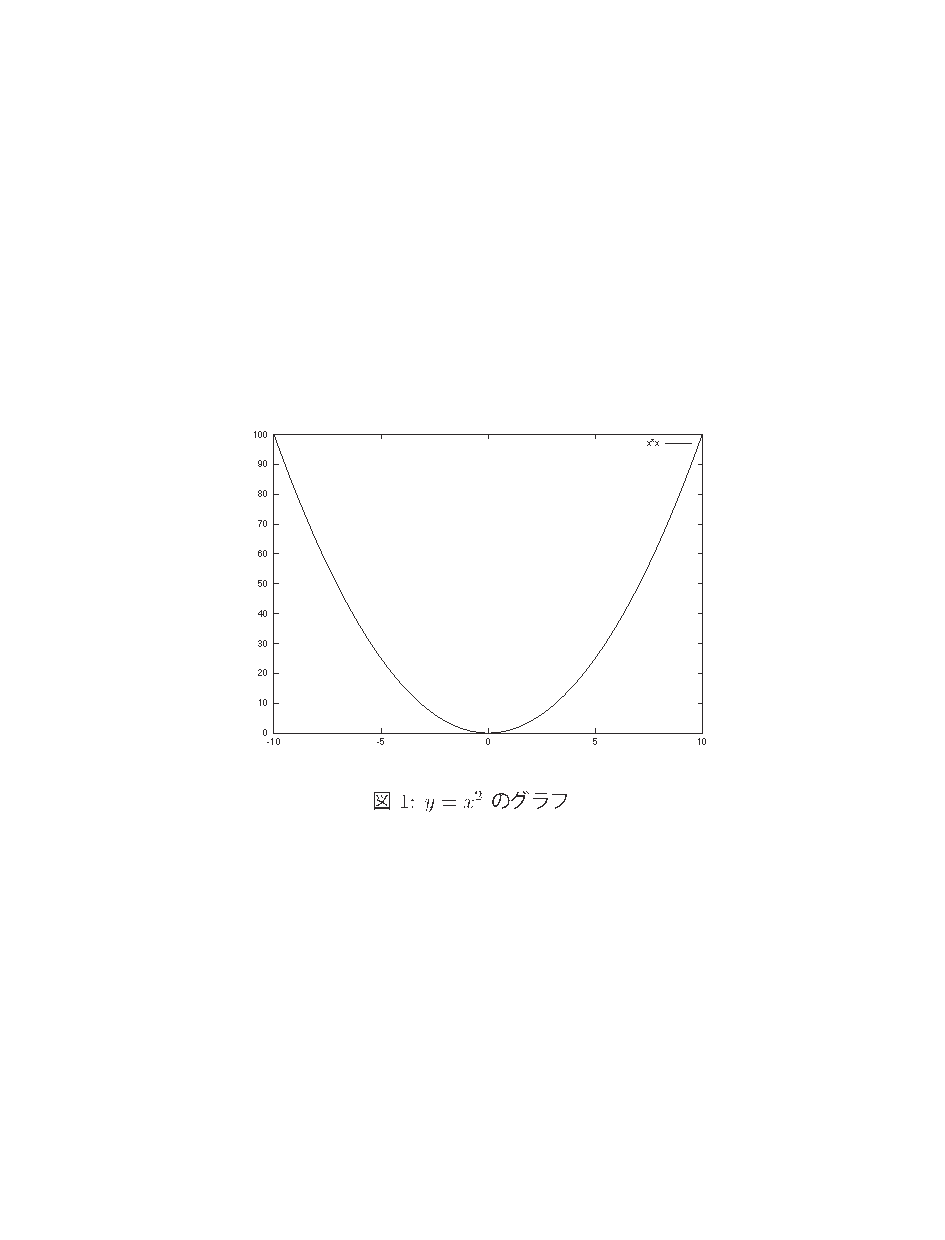
\includegraphics[width=8cm]{figure.pdf}|
\end{quotation}
という部分である。ファイル名は{\tt \{\}}の中で指定する。また \texttt{width=8cm} という記述により図の横幅を指定している。図の表題も表のときと同じく \verb|\caption| コマンドを使う。

\LaTeX は図表を自動的に適切な位置に配置してくれるが、\verb|begin{figure}| の後に \texttt{[h]} を付けると、その場に配置することができる。それでもうまくいかない場合には、\texttt{here.sty}を使い、\textbf{例題 \ref{reidai:latex:here}}のように\verb|begin{figure}| の後に \texttt{[H]} を付けることにより、強制的に指定の位置に配置することも出来る。
\begin{reidai}
\label{reidai:latex:here}
\begin{verbatim}
\documentclass{jarticle}
\usepackage{graphicx}
\usepackage{here}

\begin{document}
\begin{figure}[H]
  \begin{center}
    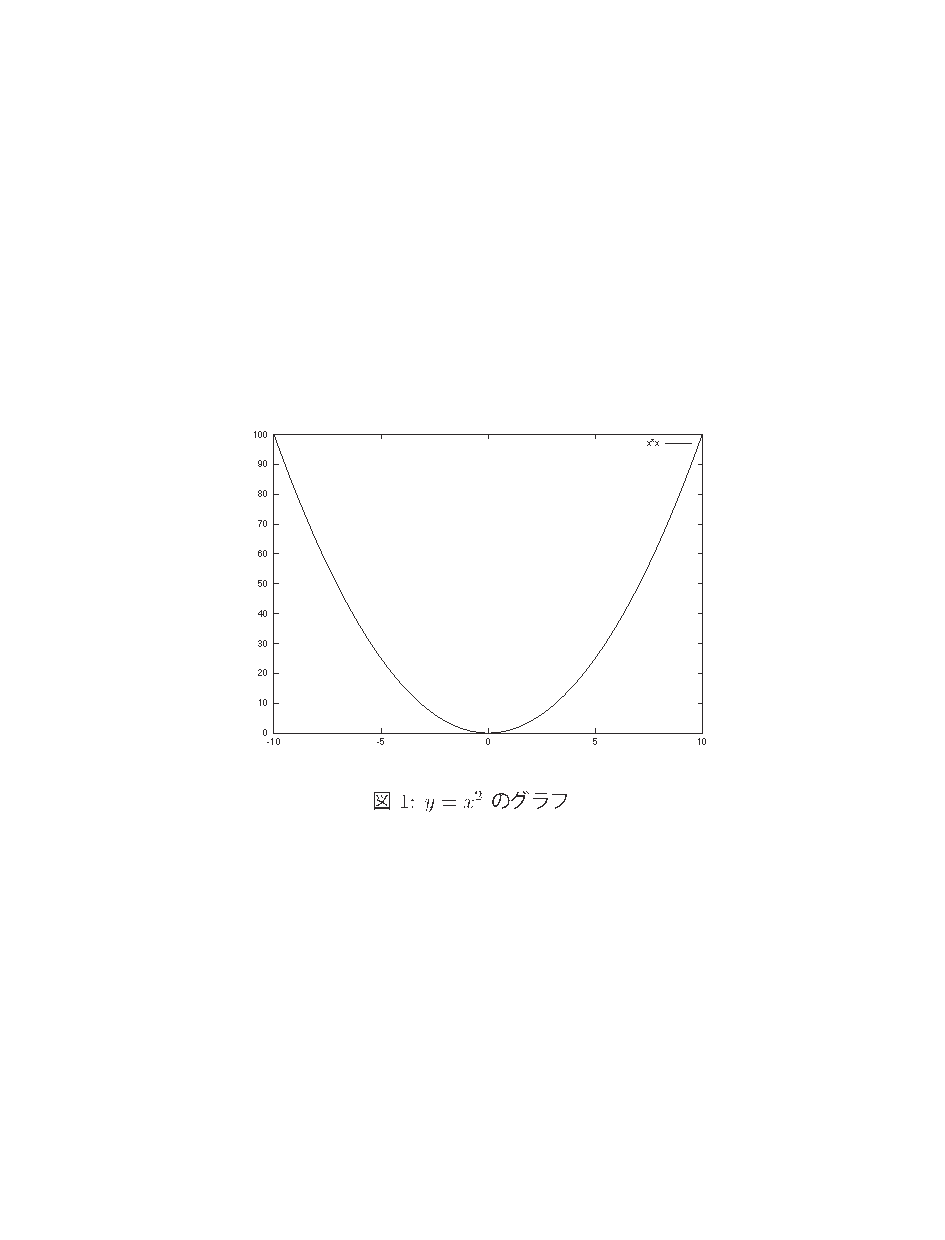
\includegraphics{figure.pdf}
    \caption{$y = x^2$ のグラフ}
  \end{center}
\end{figure}
\end{document}
\end{verbatim}
\end{reidai}

\subsection{図の回転}
\label{sec:latex:rotate_pdf}

貼り込みたいファイル中の図が 90 度回転してしまっていることがある。\LaTeX では図を貼り込むときに回転させることができる。
\begin{reidai}
\begin{verbatim}
  \rotatebox{-90}{
    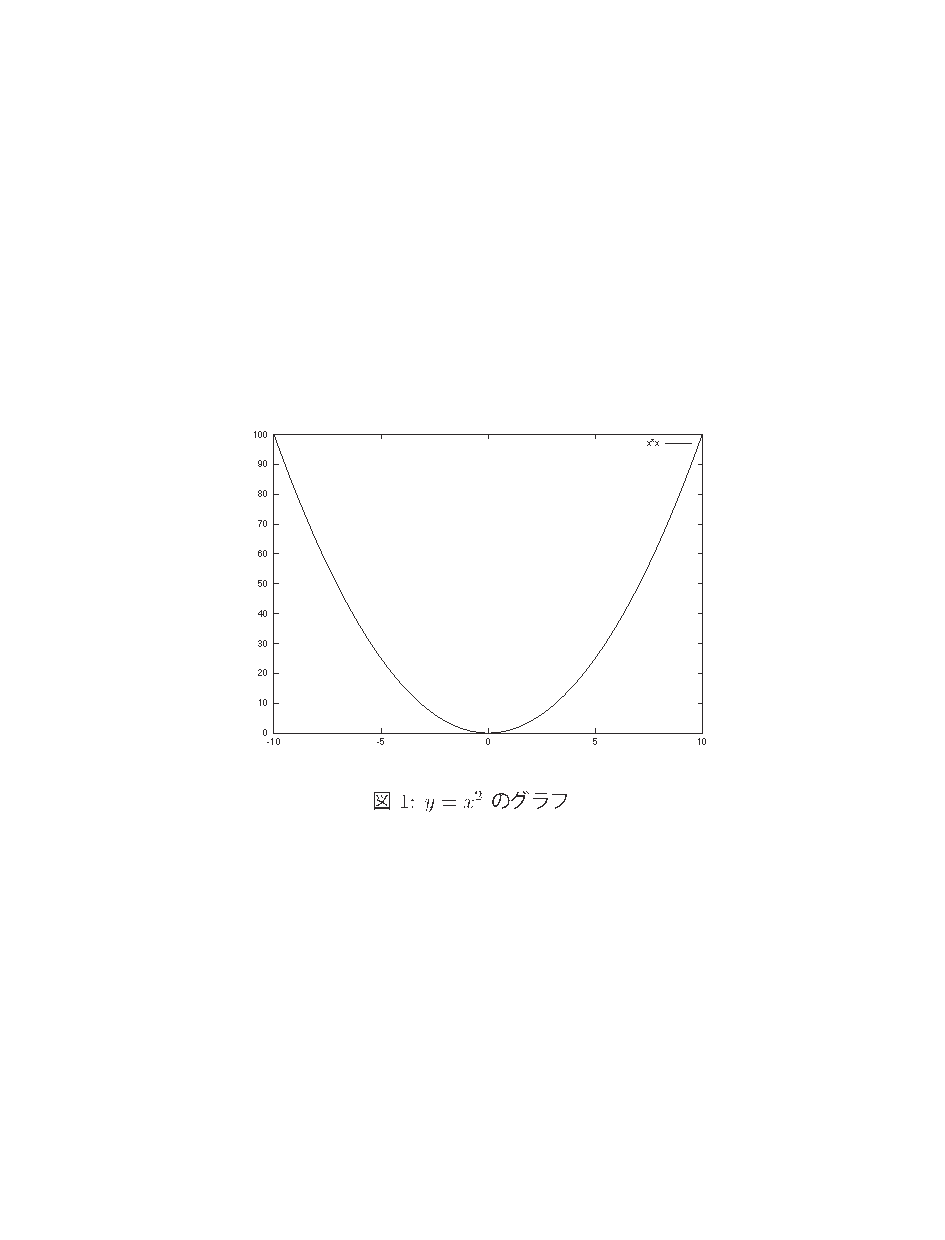
\includegraphics[width=8cm]{figure.pdf}
  }
\end{verbatim}
\end{reidai} \noindent
\vspace*{-1.5em}
\begin{kekka}
  \begin{center}
    \rotatebox{-90}{
      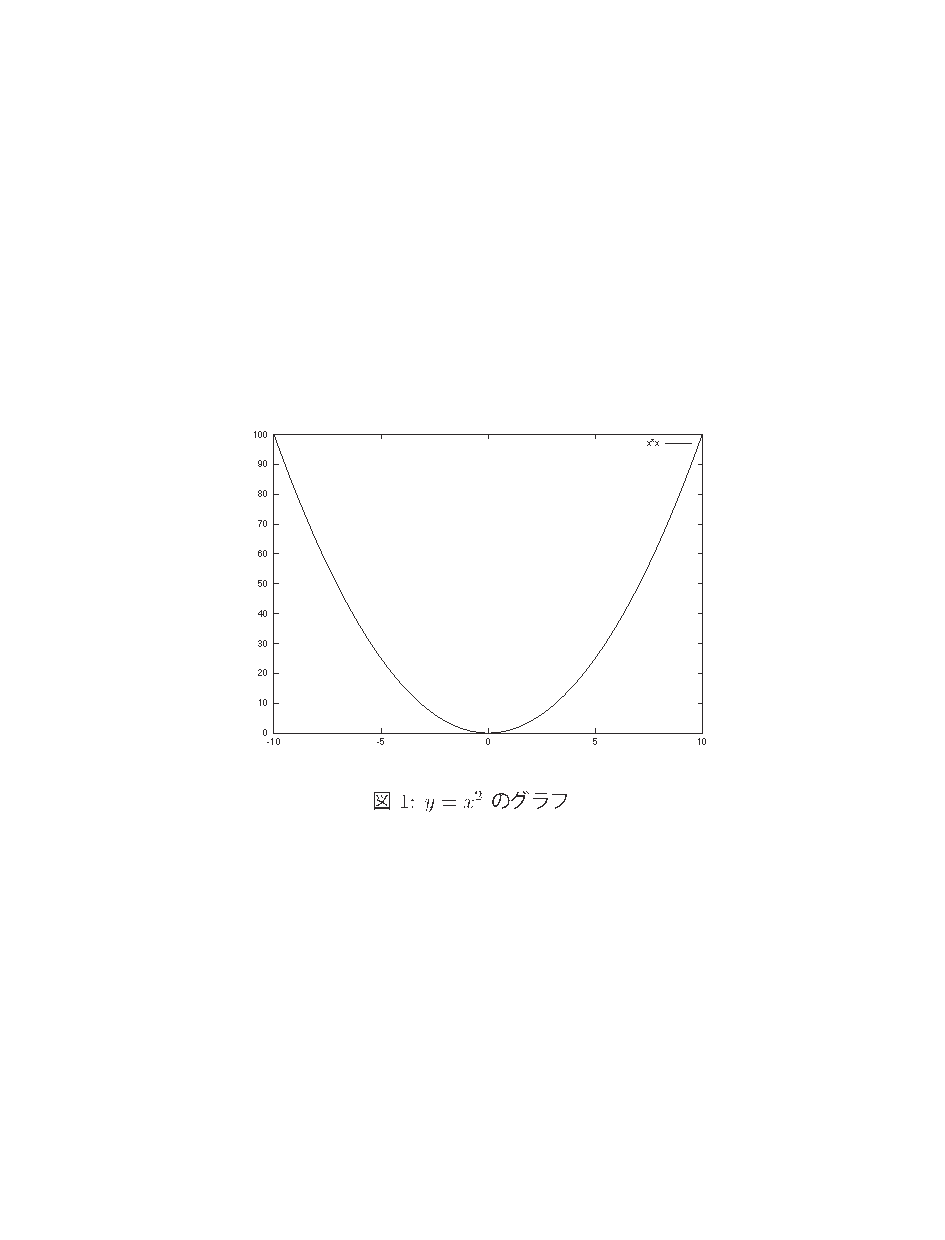
\includegraphics[width=8cm]{figure.pdf}
    }
  \end{center}
\end{kekka} \noindent
このように、 \verb|\rotatebox{-90}| を使うことにより、図を -90 度回転させることができる。


\paragraph{この節のまとめ}

\begin{itemize}
\item \LaTeX の文章には、ポストスクリプトあるいはPDF形式の図を貼り込める。
\item 実際に図を貼り込むには雛型を使う。
\item 貼り込む図を回転させるには \verb|\rotatebox{角度}{}| を使う。
\end{itemize}

\section{参照と参考文献}
\label{sec:latex:ref_and_bib}

\subsection{参照}
\label{sec:latex:reference}

\LaTeX には、数式や表、図に付いた番号を簡単に参照する機能が用意されている。まずは具体例から見ていこう。
\begin{reidai}
\label{reidai:latex:noref}
\begin{verbatim}
媒質中を物質が通過するとき、チェレンコフ光が発生するための条件は
\begin{equation}
n > \frac{1}{\beta} = \sqrt{1+\left(\frac{m}{p}\right)^{2}}
\end{equation}
である。ただし式(1) において、
$n$ は媒質の屈折率、$m$ は物質の質量、$p$ は物質の運動量である。
\end{verbatim}
\end{reidai} \noindent
この清書結果は次のようになる。
\begin{kekka}
  媒質中を物質が通過するとき、チェレンコフ光が発生するための条件は
  \begin{equation}
    n > \frac{1}{\beta} = \sqrt{1+\left(\frac{m}{p}\right)^{2}}
  \end{equation}
  である。ただし式(1) において、
  $n$ は媒質の屈折率、$m$ は物質の質量、$p$ は物質の運動量である。\\
\end{kekka} \noindent
\textbf{例題 \ref{reidai:latex:noref}} ではチェレンコフ光の発生条件の式を
本文中に「式(1)」とハードコーティングしている。

さて、 \textbf{例題 \ref{reidai:latex:noref}} の式の前に別の式を挿入することになったとする。すると、式の番号はすべて 1 つずつ繰り下がるので、文章中で「式(1)」と書いているところをすべて「式(2)」に書き直さなければならない。このような番号の付け替えを手で行うのはとても大変であるし、間違いが起こりやすい。

こういった手間を省くために、 \LaTeX には数式や表・図に名前を
割り当てる機能が用意されている。
\begin{reidai}
\label{reidai:latex:ref}
\begin{verbatim}
媒質中を物質が通過するとき、チェレンコフ光が発生するための条件は
\begin{equation}
n > \frac{1}{\beta} = \sqrt{1+\left(\frac{m}{p}\right)^{2}} \label{cherenkov}
\end{equation}
である。ただし式(\ref{cherenkov}) において、
$n$ は媒質の屈折率、$m$ は物質の質量、$p$ は物質の運動量である。
\end{verbatim}
\end{reidai} \noindent
\textbf{例題 \ref{reidai:latex:ref}} は\textbf{例題 \ref{reidai:latex:noref}} と
同じ清書結果を与える。

数学環境中で \verb|\label| を使うとその数式に名前が付けられる。付ける名前は \verb|\label| の後の \verb|\{\}| の中に記述する。\textbf{例題 \ref{reidai:latex:ref}} では \texttt{cherenkov} という名前が付けられている。

さて、名前の付けられた数式をその名前で参照すると、その箇所が数式の番号に展開される。参照は \verb|\ref| コマンドを使う。\textbf{例題 \ref{reidai:latex:ref}} では \verb|\ref{cherenkov}| として参照している。\verb|\label{cherenkov}| によって名前付けした数式の番号は 1 だったので、 \verb|\ref{cherenkov}| の参照によってこれが 1 に展開されることになる。

以下に参照の例を挙げておく。
\begin{reidai}
\begin{verbatim}
本年度の遠足について、以下のとおり決定いたしましたのでお知らせします。
\begin{table}
  \begin{center}
    \caption{遠足の目的地(学年別)}
    \label{destination}
    \begin{tabular}{|l|l|}
      \hline
      学年 & 目的地 \\
      \hline \hline
      4 年生 & 近くにある公園 \\
      \hline
      5 年生 & 遠くにある公園 \\
      \hline
      6 年生 & かなり遠くにある公園 \\
      \hline
    \end{tabular}
  \end{center}
\end{table}
表 \ref{destination} をよく読んで自分の目的地をきちんと確認し、
遠足の目的地に相応しい準備をするように心がけてください。

なお、おやつの持参は
\begin{equation}
\sum^{全おやつ} 各おやつの購入金額 \le 500 円 \label{oyatu}
\end{equation}
を条件とします。
ただし、バナナは 式(\ref{oyatu})にかかわらず好きなだけ持参して差しつかえありません。
\end{verbatim}
\end{reidai}
\vspace*{-1.5em}
\begin{kekka}
本年度の遠足について、以下のとおり決定いたしましたのでお知らせします。
  \begin{center}
    表1: 遠足の目的地(学年別) \\
    \begin{tabular}{|l|l|}
      \hline
      学年 & 目的地 \\
      \hline \hline
      4 年生 & 近くにある公園 \\
      \hline
      5 年生 & 遠くにある公園 \\
      \hline
      6 年生 & かなり遠くにある公園 \\
      \hline
    \end{tabular}
  \end{center}
表1をよく読んで自分の目的地をきちんと確認し、
遠足の目的地に相応しい準備をするように心がけてください。

なお、おやつの持参は
\begin{equation}
\sum^{全おやつ} 各おやつの購入金額 \le 500 円
\end{equation}
を条件とします。
ただし、バナナは式(1)にかかわらず好きなだけ持参して差しつかえありません。
\end{kekka}


\subsection{参考文献}
\label{sec:latex:bibliography}

論文やレポートでは、通常、末尾に参考文献リストを付ける。
参考文献の番号も数式などと同じように自動的に振ることができる。
\begin{reidai}
\begin{verbatim}
第 1 象限内の複素数 $z$ について、
\begin{equation}
w(z) \equiv \mathrm{e}^{-z^2}\mathrm{erfc}(z)
\end{equation}
を近似的に計算するアルゴリズムが存在し \cite{wofz}、
その計算誤差は $10 ^ {-10}$ 以下である。
\\
このアルゴリズムは、 BELLE 実験 \cite{BELLE} で使用するプログラムの内部で利用されている。

...

\begin{thebibliography}{99}
\bibitem{wofz}
  Walter Gautschi, Comm ACM. \textbf{12} 635, (1969) 
\bibitem{BELLE}
  The BELLE Collaboration, KEK Report 95-1 (1995)
\end{thebibliography}
\end{verbatim}
\end{reidai}
\setcounter{equation}{0}
\vspace*{-1.5em}
\begin{kekka}
  \hspace*{0.3cm}第 1 象限内の複素数 $z$ について、
  \begin{equation}
    w(z) \equiv \mathrm{e}^{-z^2}\mathrm{erfc}(z)
  \end{equation}
  を近似的に計算するアルゴリズムが存在し[1]、
  その計算誤差は $10 ^ {-10}$ 以下である。
  \\
  このアルゴリズムは、 BELLE 実験[2]で使用するプログラムの
  内部で利用されている。

  \dots

  \noindent {\bf \Large 参考文献} \\

  \noindent [1] Walter Gautschi, Comm ACM. \textbf{12} 635, (1969)

  \noindent [2] The BELLE Collaboration, KEK Report 95-1 (1995)
\end{kekka} \noindent
文章中に書く \verb|\cite| では引用する論文の名前を指定する。論文の名前は自分が覚えやすいものであれば何でも構わないが、\verb|\bibitem| によって名前が定義されている必要がある。\verb|\bibitem| は \verb|\begin{thebibliography}| と \verb|\end{thebibliography}| とで囲まれた領域に書く。この領域は清書すると参考文献の章となる。
\verb|\bibitem| に続く {\tt \{\}} の中には自分で決めた論文名を書く。この名前が \verb|\cite| によって参照されることになる。その後あとには、その論文の著者名や収録されている雑誌名などを書く。ここに書いたことは、参考文献の章が清書されるときにそのまま印刷される。

\verb|\cite| と \verb|\ref| を、 \verb|\bibitem| と \verb|\label| を
それぞれ対応付けて覚えておこう。


\subsection{コンパイル}
\label{sec:latex:compile}

参照を含むソースファイルを \LaTeX で処理するときは、\texttt{platex} コマンドを何回か実行する必要がある。これは、 \texttt{platex} が参照関係を解決することが、 1 回のコマンド実行だけではできないからである。参照が解決できていない状態では、展開されるべき参照の部分が ?? と表示される。\texttt{platex} の実行を何回か繰り返し、 ?? になっている参照がなくなったことを確認すること。

\paragraph{この節のまとめ}

\begin{itemize}
\item 数式や表、図には \verb|\label{名前}| で名前を付けられる。
\item 数式などに付けられた番号は、 \verb|\label{名前}| で付けた名前を手掛かりにして \verb|\ref{名前}| と書くことで参照できる。
\item 参考文献は \verb|\cite{論文名}| のようにして参照する。
\item 参考にした論文は、 \verb|\begin{thebibliography}| から
    \verb|\end{thebibliography}| までの領域に書く。
\item 論文は \verb|\bibitem{論文名}| 著者、雑誌名 \dots のように列挙する。
\item 参照を含むソースファイルに対しては、何回か \texttt{platex} コマンドを
  実行する必要がある。
\end{itemize}


%\chapter{数値計算アルゴリズム}
%\input{algorithm}

%\chapter{Mathematica見よう見まね}

%\addcontentsline{toc}{chapter}{\bibname}
%\bibliography{main}
%\begin{thebibliography}{99}
%\end{thebibliography}

\end{document}
